\chapter{User documentation}
\label{ch:user}

\section{General Requisite}

The application is for the internal usage within SAP for the parcel collection service providing to the employees. The solution consists of 6 applications as tiles on the Fiori launchpad: \textbf{My packages}, \textbf{Pickup packages}, \textbf{Register Packages}, \textbf{Manage packages}, \textbf{Manage Companies} and \textbf{Manage Storages} partitioned into 3 sections: \textbf{My Home}, \textbf{Pacel Handling}, \textbf{Administration}, as shown in the diagram.

\begin{figure}[H]
	\centering
	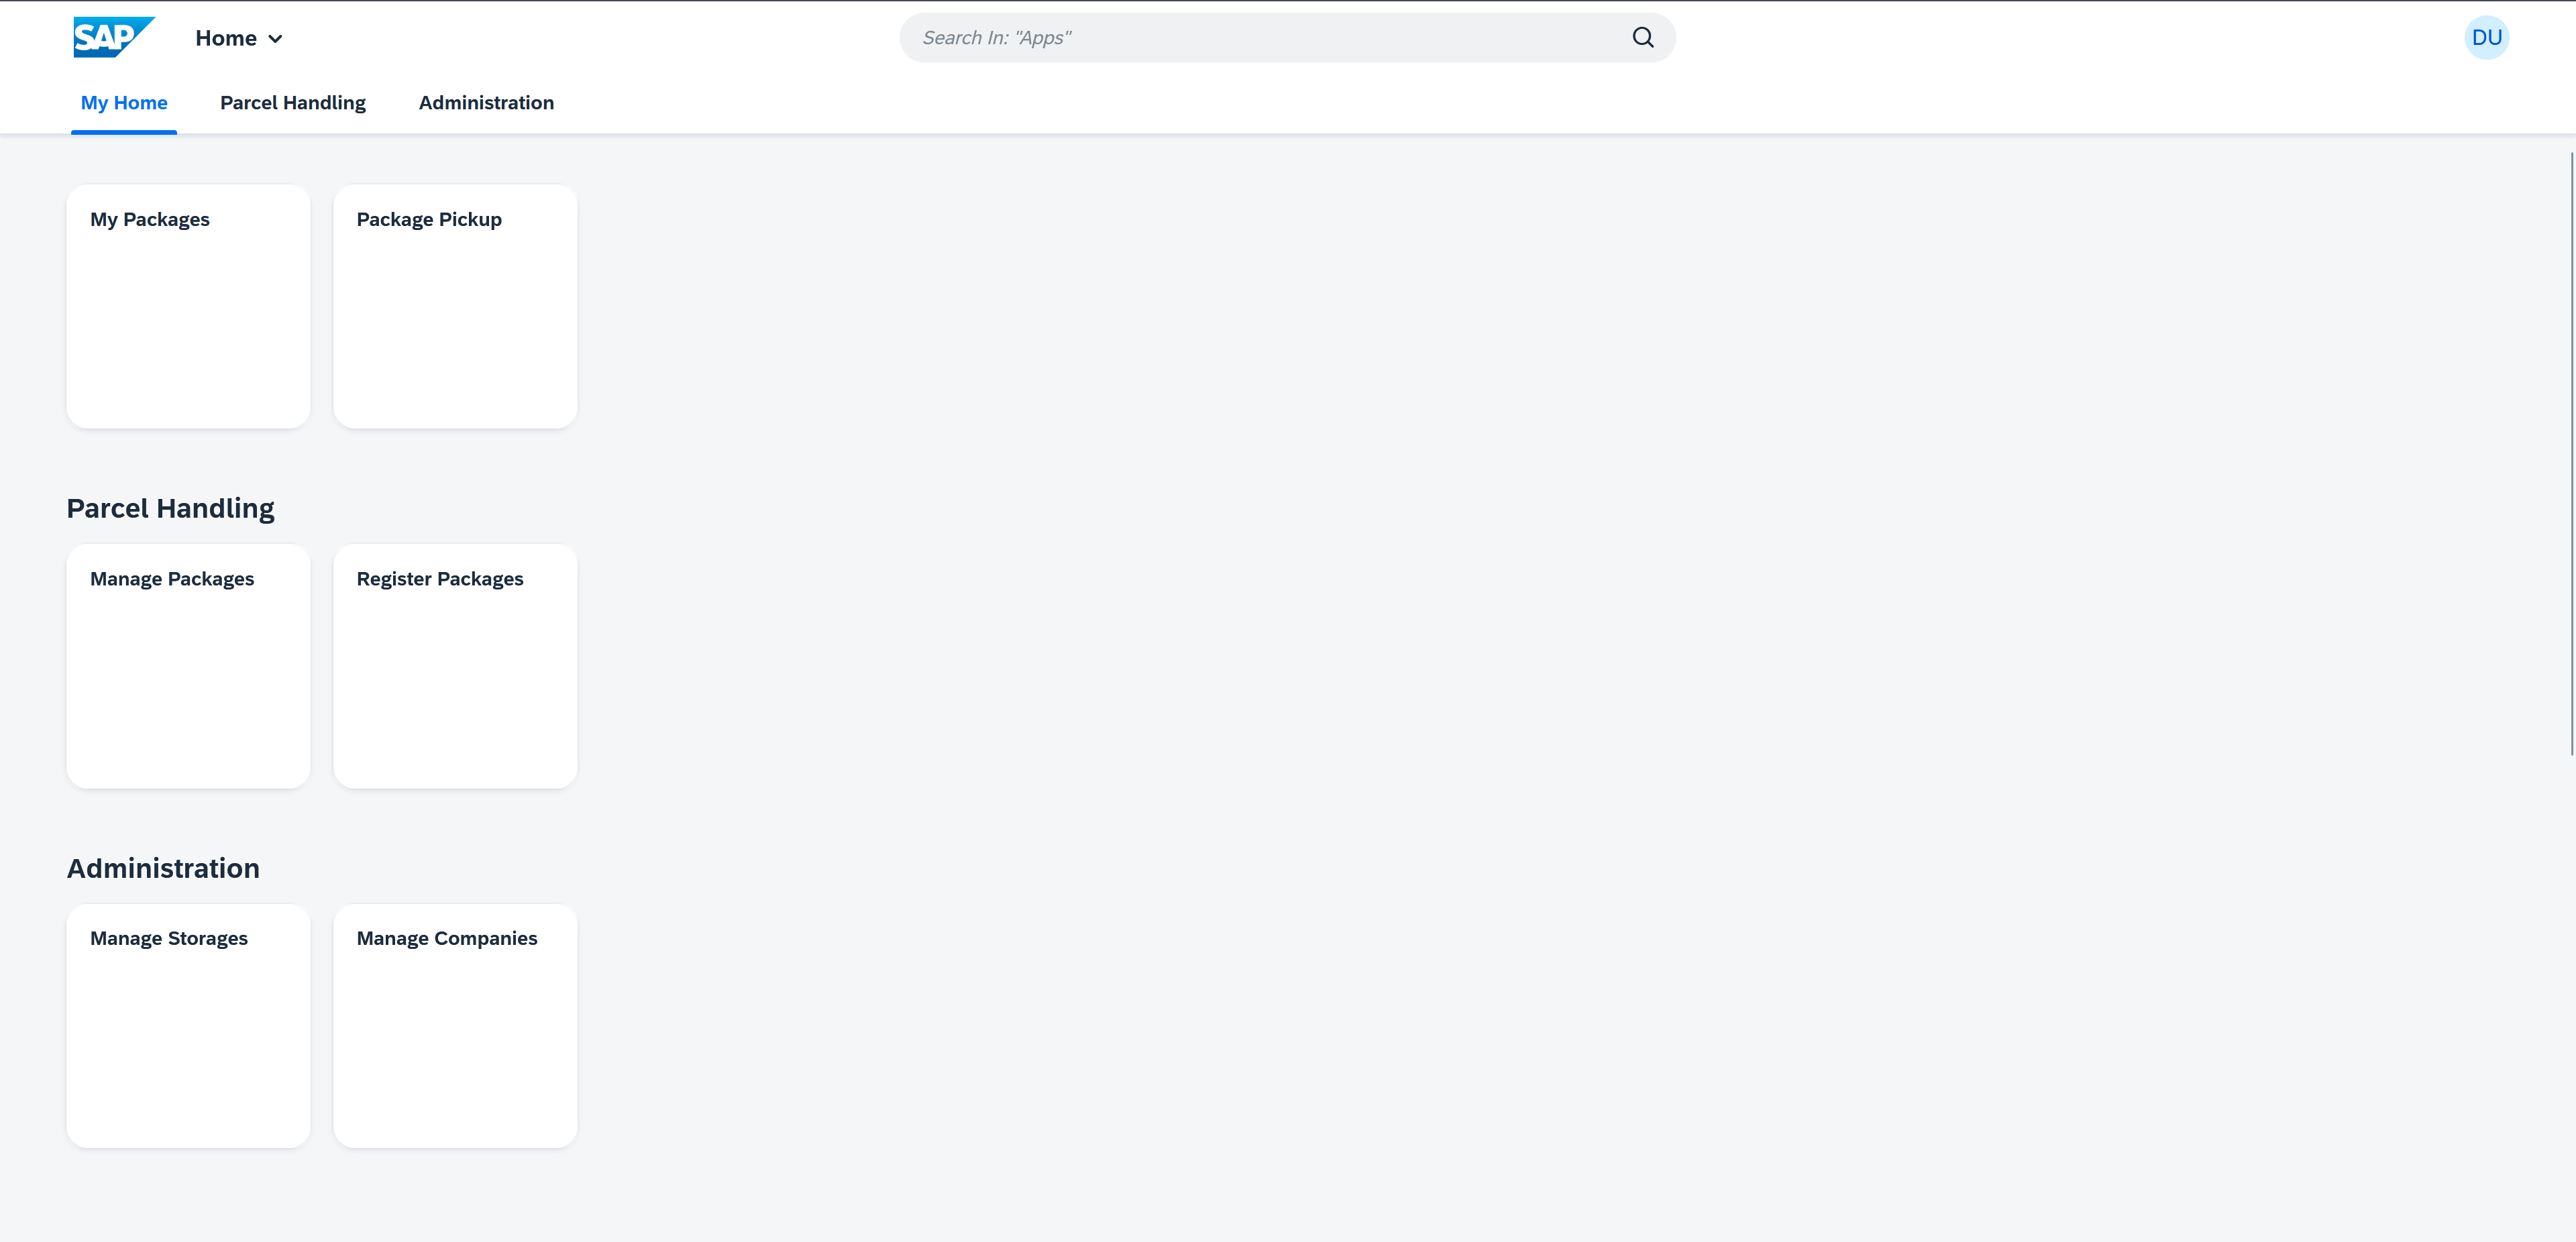
\includegraphics[width=1\linewidth]{images/user_doc/overviews/sandbox.png}
	\caption{Application Launch Screen}
	\label{fig:ApplicationLaunchScreen}
\end{figure}


In order to use any of the application, one has to hold an SAP registered device (computer/tablet/phone) and is able to use a supported browser with stable internet connection. In order to use \textbf{Pickup packages} application, one has to hold an SAP registered smart phone. 

In order to mock use the application in local environment, please move the the developer chapter. 

Four different roles are specified for the application and one is limited to dedicated usage of the applications, depends on the role. In the coming sections the usage guides are documented partitioned by the roles. Hereby lists the meaning of each role under the thesis context:

\begin{description}
	\item[End User] any SAP employee who holds an SAP registered device and would like to use the parcel collection service.
	\item[Receptionist] Registered receptionist (in database) working at the reception and is responsible to serve the parcel collection service.
	\item[Facility Manager] Authorised user who is responsible for maintaining the delivery companies and storage slots information.
	\item[Administrator] The master user who can access to any of the applications.
\end{description}

In case one is accessing the applications through browser from BTP platform, the login process is done automatically. Otherwise, if one is running the application locally, a browser pop up will appear and mock user should be entered. The different mock user login info can be find in the developer documentation security chapter.

\begin{figure}[H]
	\centering
	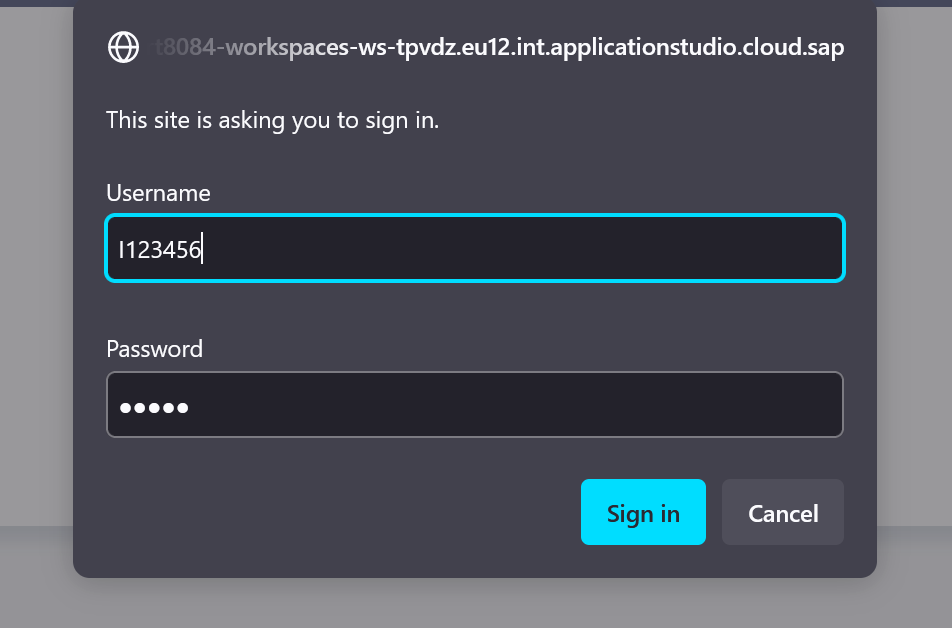
\includegraphics[height=200pt]{images/user_doc/overviews/localLogin.png}
	\caption{Local Login Pop Up}
	\label{fig:LocalLoginPopUp}
\end{figure}

In the case of any user trying to accessing an unauthorised application, connection will fail.

\begin{figure}[H]
	\centering
	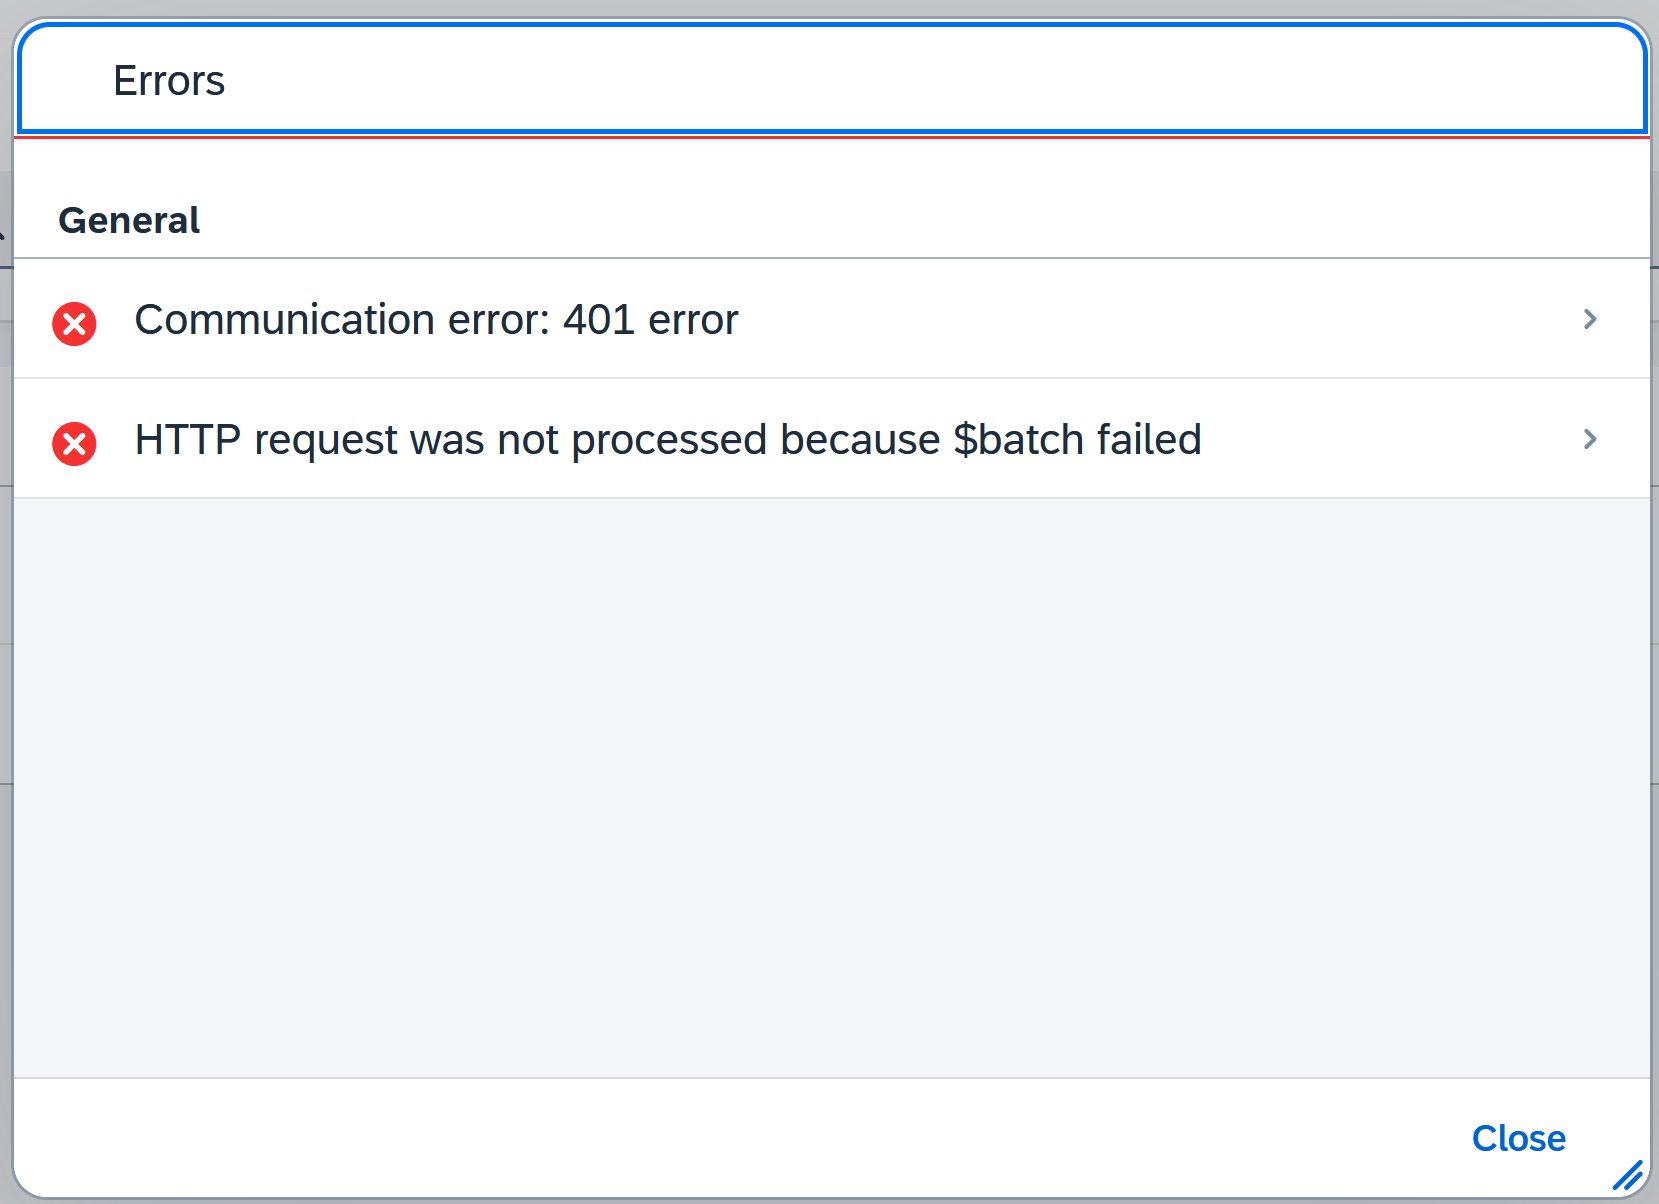
\includegraphics[width=1\linewidth]{images/user_doc/overviews/ConnectionError1.png}
	\caption{Illegal Access to Unauthorised Applications - Possible Error}
	\label{fig:IllegalAccesstoUnauthorised Applications}
\end{figure}

\pagebreak

\section{End User}

As a logged in \textbf{End User}, one is granted to access the two applications under the \textbf{My Home} section, namely \textbf{My Packages} and \textbf{Package Pickup}. One can quick jump to the section by left clicking the "My Home" tab. One can enter the application by left click the tiles.

\begin{figure}[H]
	\centering
	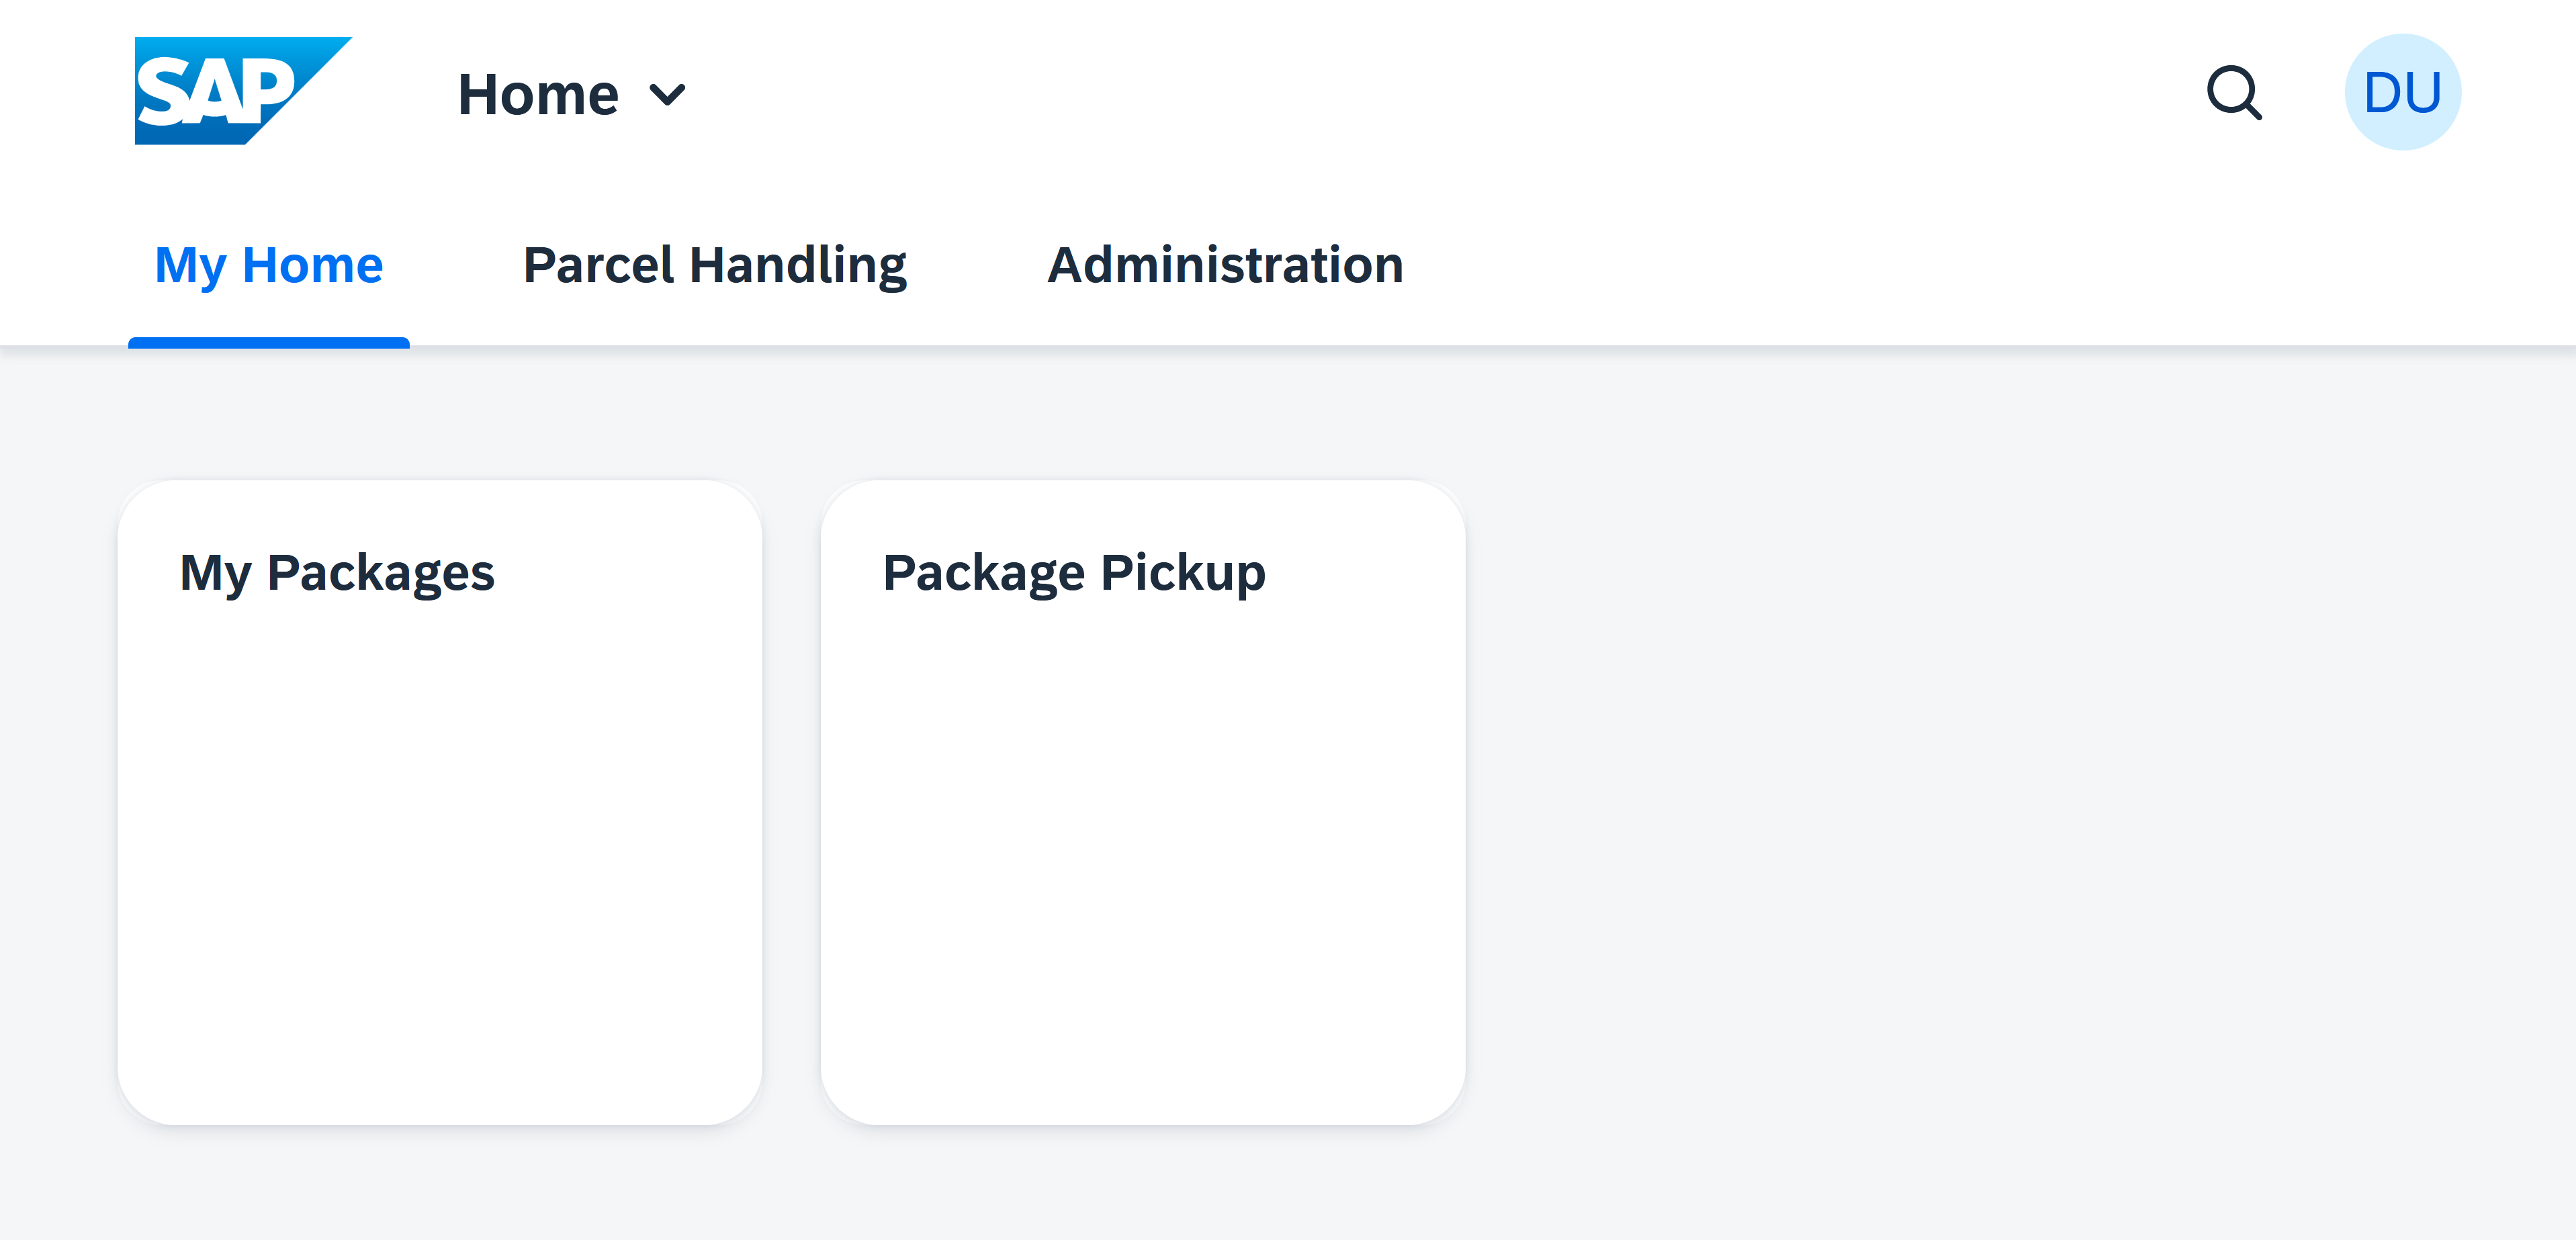
\includegraphics[width=1\linewidth]{images/user_doc/overviews/MyHomeTab.png}
	\caption{End User Applications}
	\label{fig:EndUserApplications}
\end{figure}


% ----------------------- MY PACKAGES ----------------------------
% 
%  ---------------------------------------------------------------

\subsection{My Packages}

The \textbf{My Packages} application is here for any \textbf{End User} who would want to check his/her own packages. Both the picked up ones, or the ones still under process can be checked here. One can only see one's own confirmed packages. 

\subsubsection{Home Screen - Overview}
As an \textbf{End User}, after clicking at the application tile, is redirected to the "Home Screen", which is the main and only screen of this application. The upper part displays the search bar and the possible filters. While the lower part displays the list of packages. The information provides for each packages are: \textbf{Type} (the type of the package, existing types are newspaper, letter and normal), \textbf{Status} (the status of the package, existing status are new, confirmed and picked up), \textbf{Delivery Company} (the delivery company of the package), \textbf{Delivery Time} (the confirmation time of the package, if applicable), \textbf{Pickup Time} (the picked up time of the package, if applicable).

\begin{figure}[H]
	\centering
	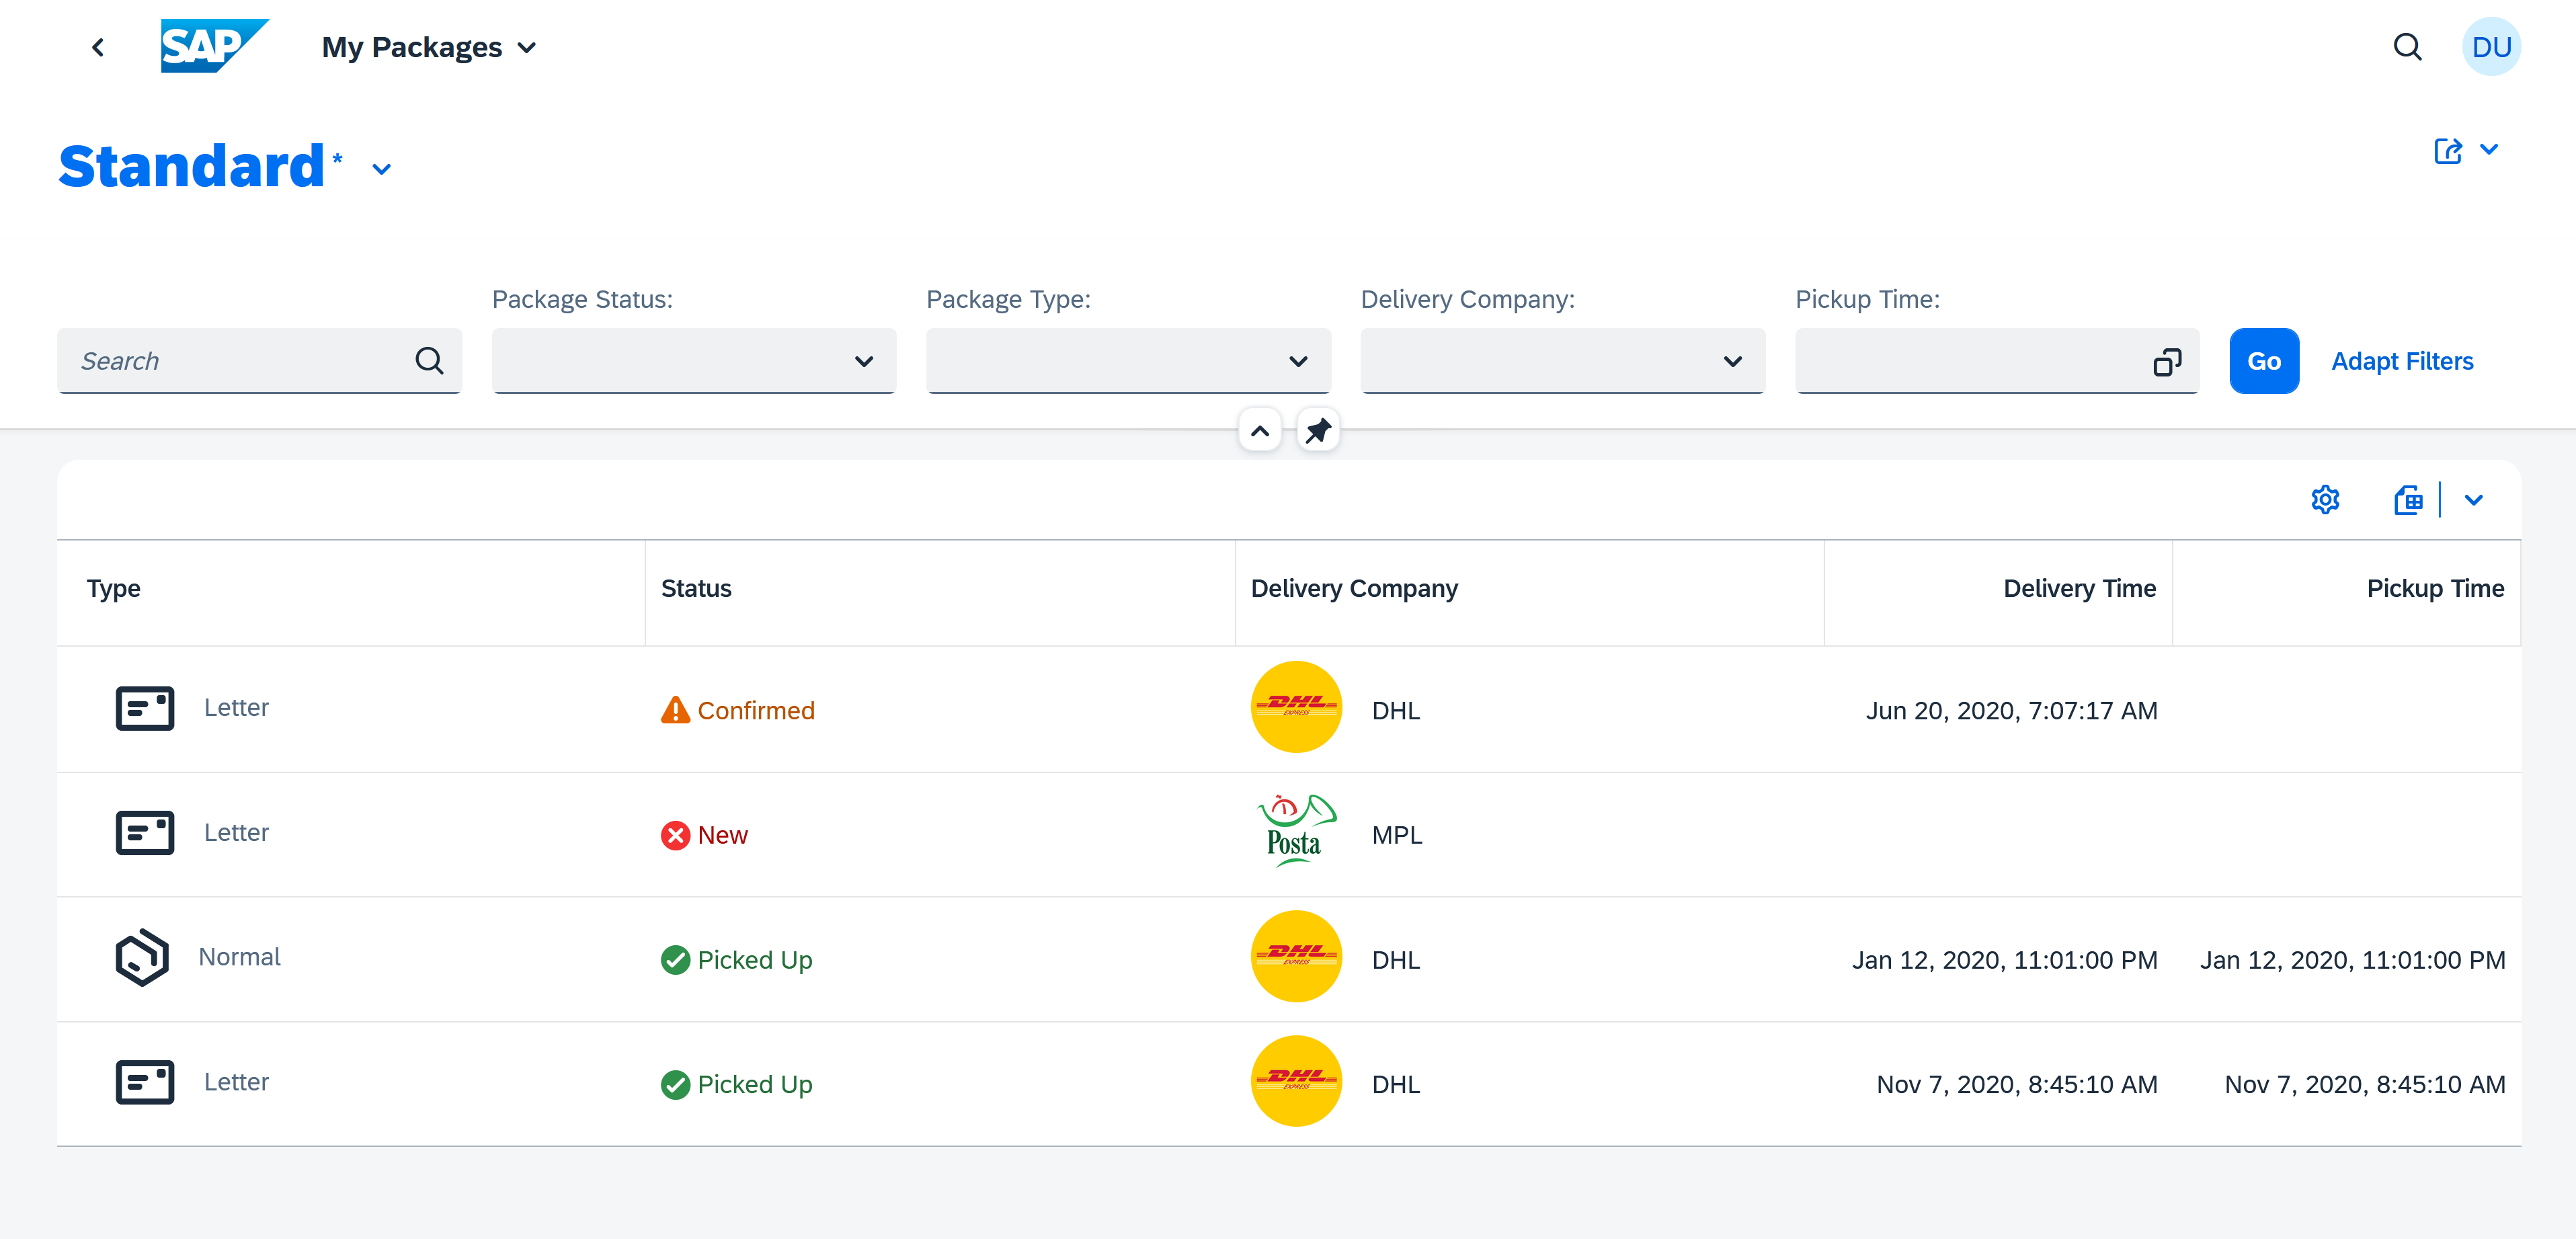
\includegraphics[width=1\linewidth]{images/user_doc/myPack/overview.png}
	\caption{History Home Screen - Overview}
	\label{fig:HistoryHome}
\end{figure}

\subsubsection{Home Screen - Filter Usage}
One can type in free text of any possible content of the column in the "Search Bar". The free text supports in-completed keywords and is case insensitive. One can use the default filters (\textbf{Status} (drop down), \textbf{Type} (drop down), \textbf{Delivery Company} (drop down) and \textbf{Pickup Time} (time entry). For drop down filters, one can click at the small drop down arrow and select zero to many options. For time entry, one shall click at the "double box" (filter help) on the right of the filter box. This will pops up a dialog, at where one can select the desired filtering option and enter the time with the clock uitility (as shown in the coming figure). One can also access to more filters (\textbf{Delivery Time} (time entry) by clicking at "Adapt Filters". WHile adjusting the filtering values, the list view is temporarily locked. After adjusting the filtering values, run the filter by clicking the "Go" Button.

\begin{figure}[H]
	\centering
	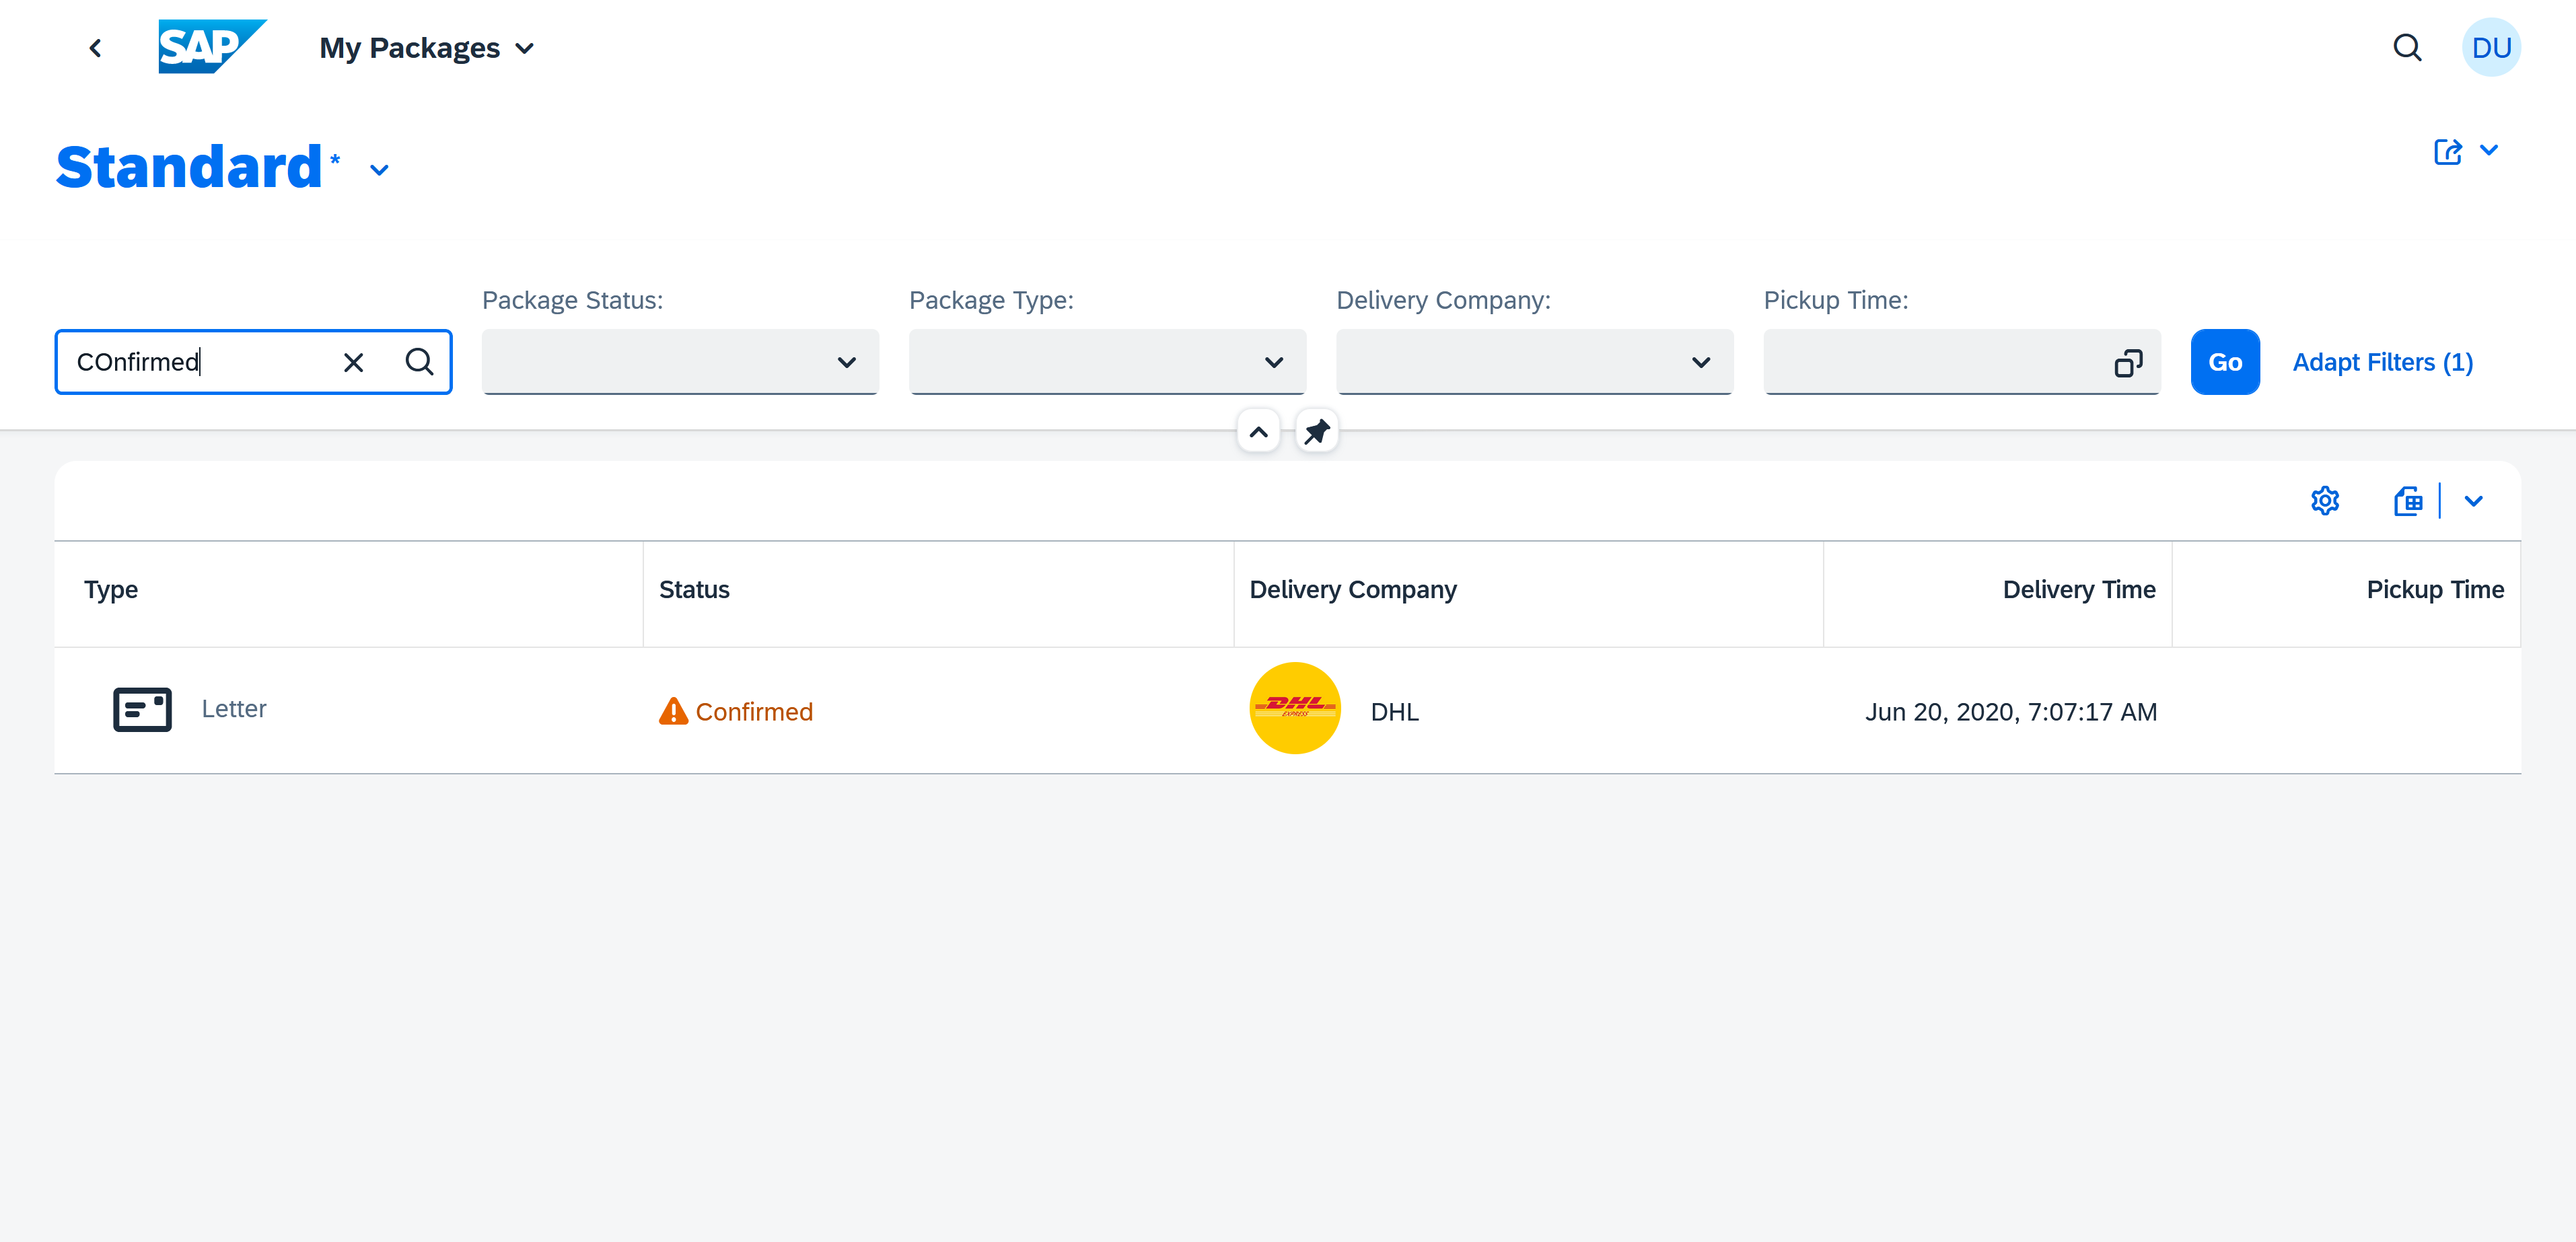
\includegraphics[width=1\linewidth]{images/user_doc/myPack/searchbar.png}
	\caption{My Package Home Screen - Search Bar}
	\label{fig:mpSearchBar}
\end{figure}


\begin{figure}[H]
	\centering
	\subcaptionbox{Status Filter}{
		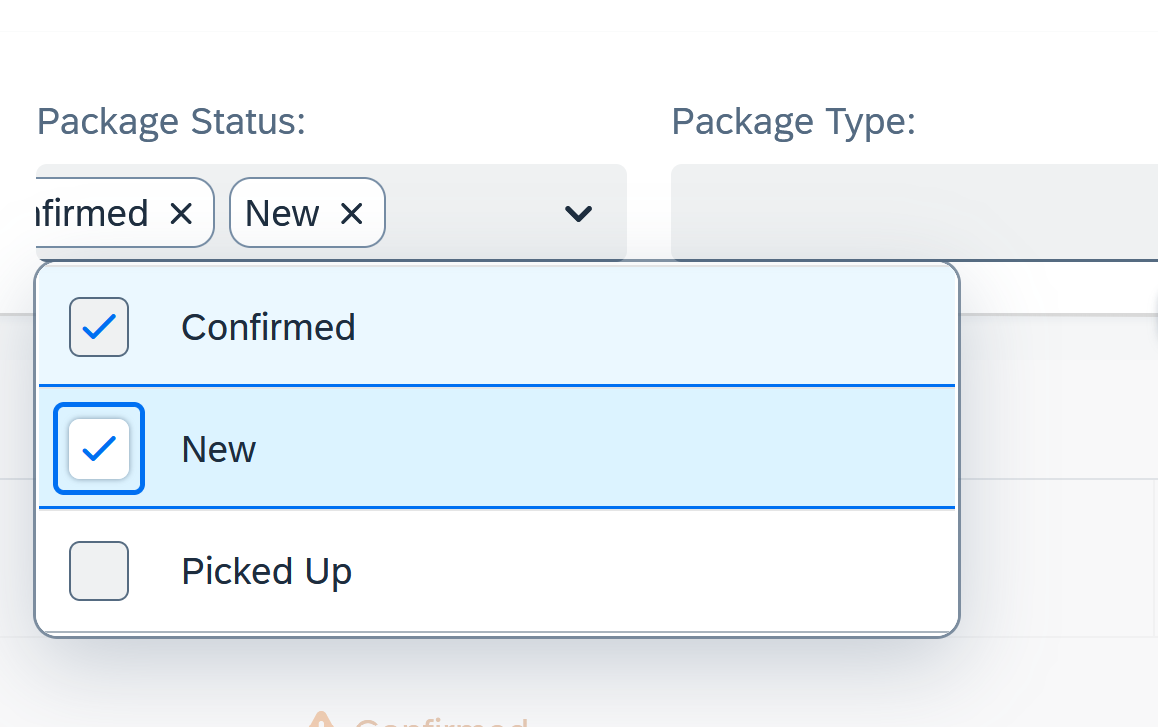
\includegraphics[width=0.45\linewidth]{images/user_doc/myPack/statusFIlter.png}}
	\hspace{5pt}
	\subcaptionbox{Type Filter}{
		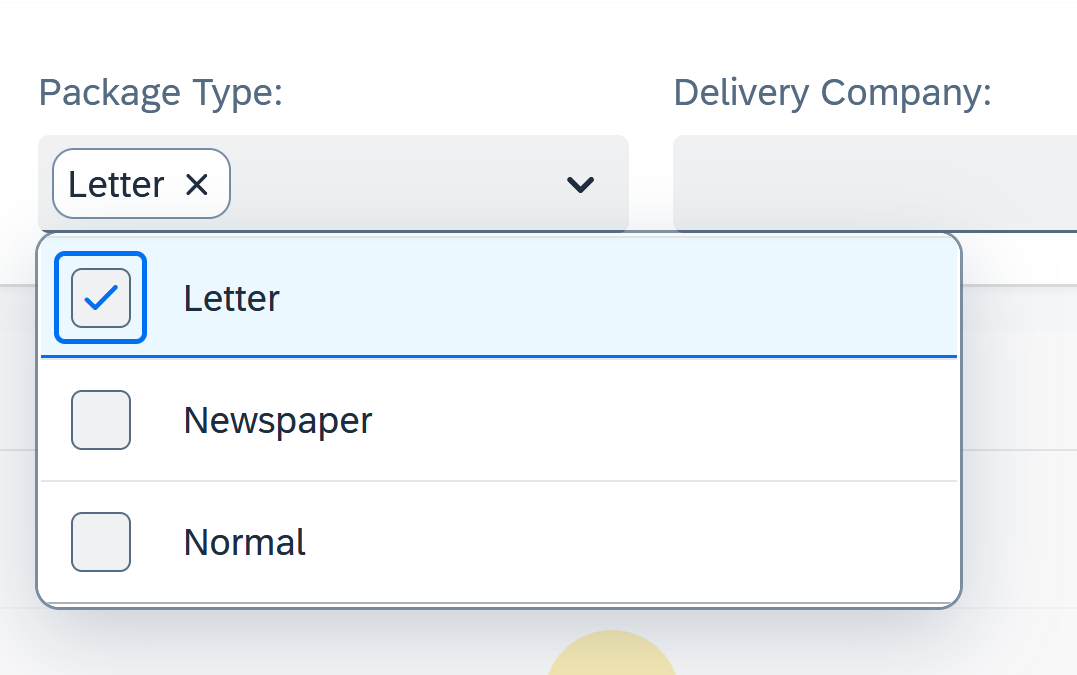
\includegraphics[width=0.45\linewidth]{images/user_doc/myPack/typeFIlter.png}}

    \subcaptionbox{Company Filter}{
		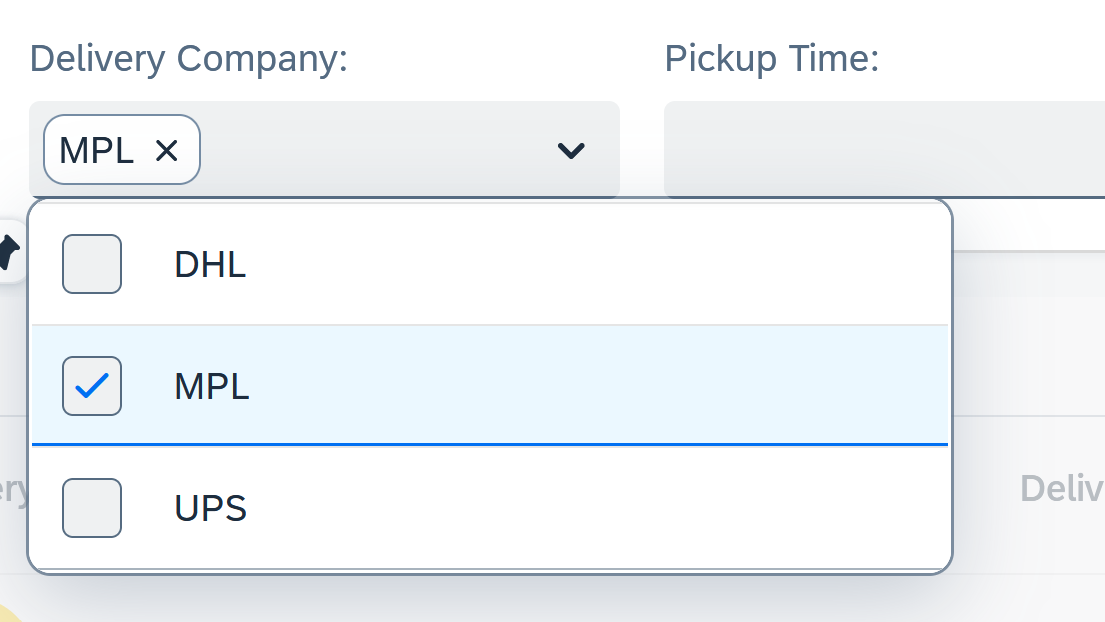
\includegraphics[width=0.45\linewidth]{images/user_doc/myPack/companyFilter.png}}
	\hspace{5pt}
	\subcaptionbox{Time Filter}{
		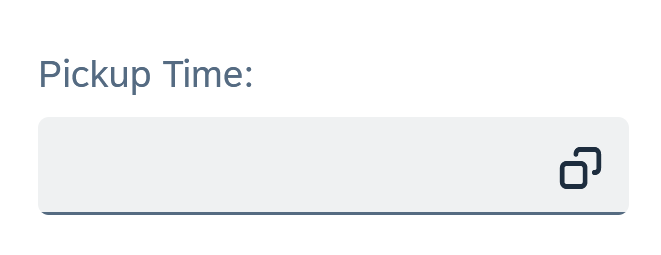
\includegraphics[width=0.45\linewidth]{images/user_doc/myPack/timeFilter.png}}
	\caption{My Package Home Screen - Default Filters}
	\label{fig:MPHomeScreen-1}
\end{figure}

\begin{figure}[H]
		\centering
	\subcaptionbox{Time Filter Options Selections}{
		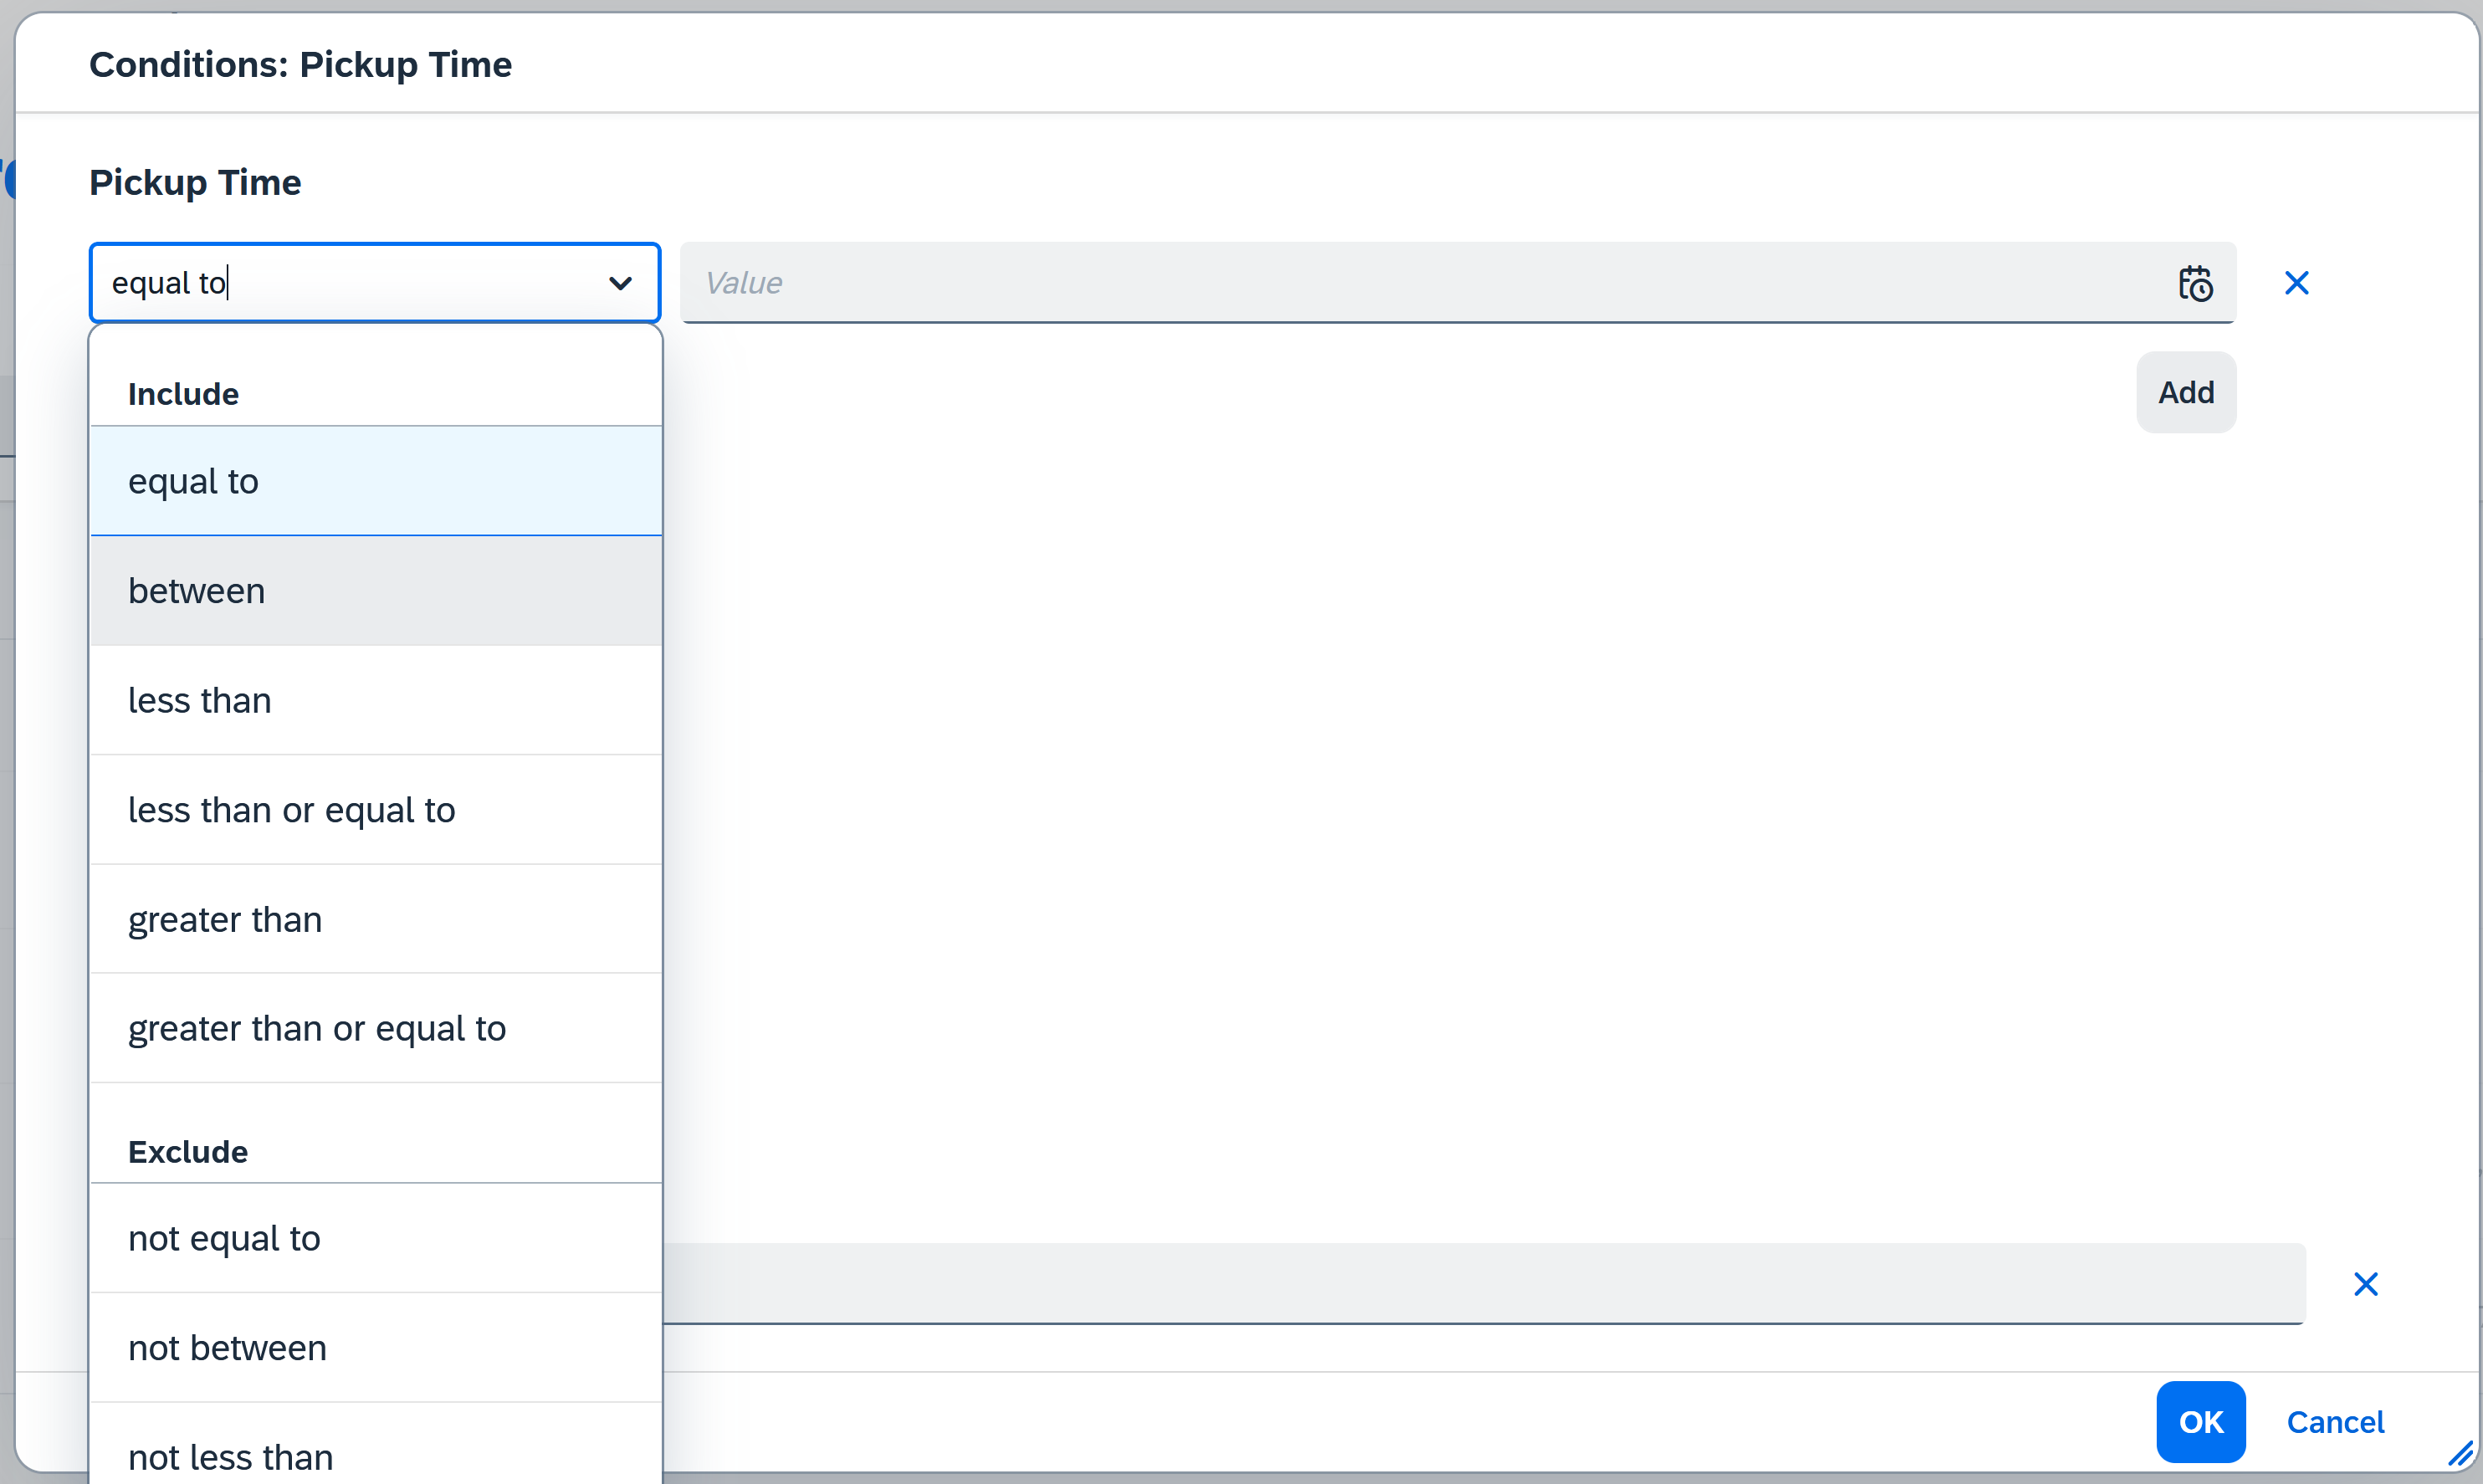
\includegraphics[width=0.45\linewidth]{images/user_doc/myPack/timeFilter_Usage1.png}}
	\hspace{5pt}
	\subcaptionbox{Time Entry}{
		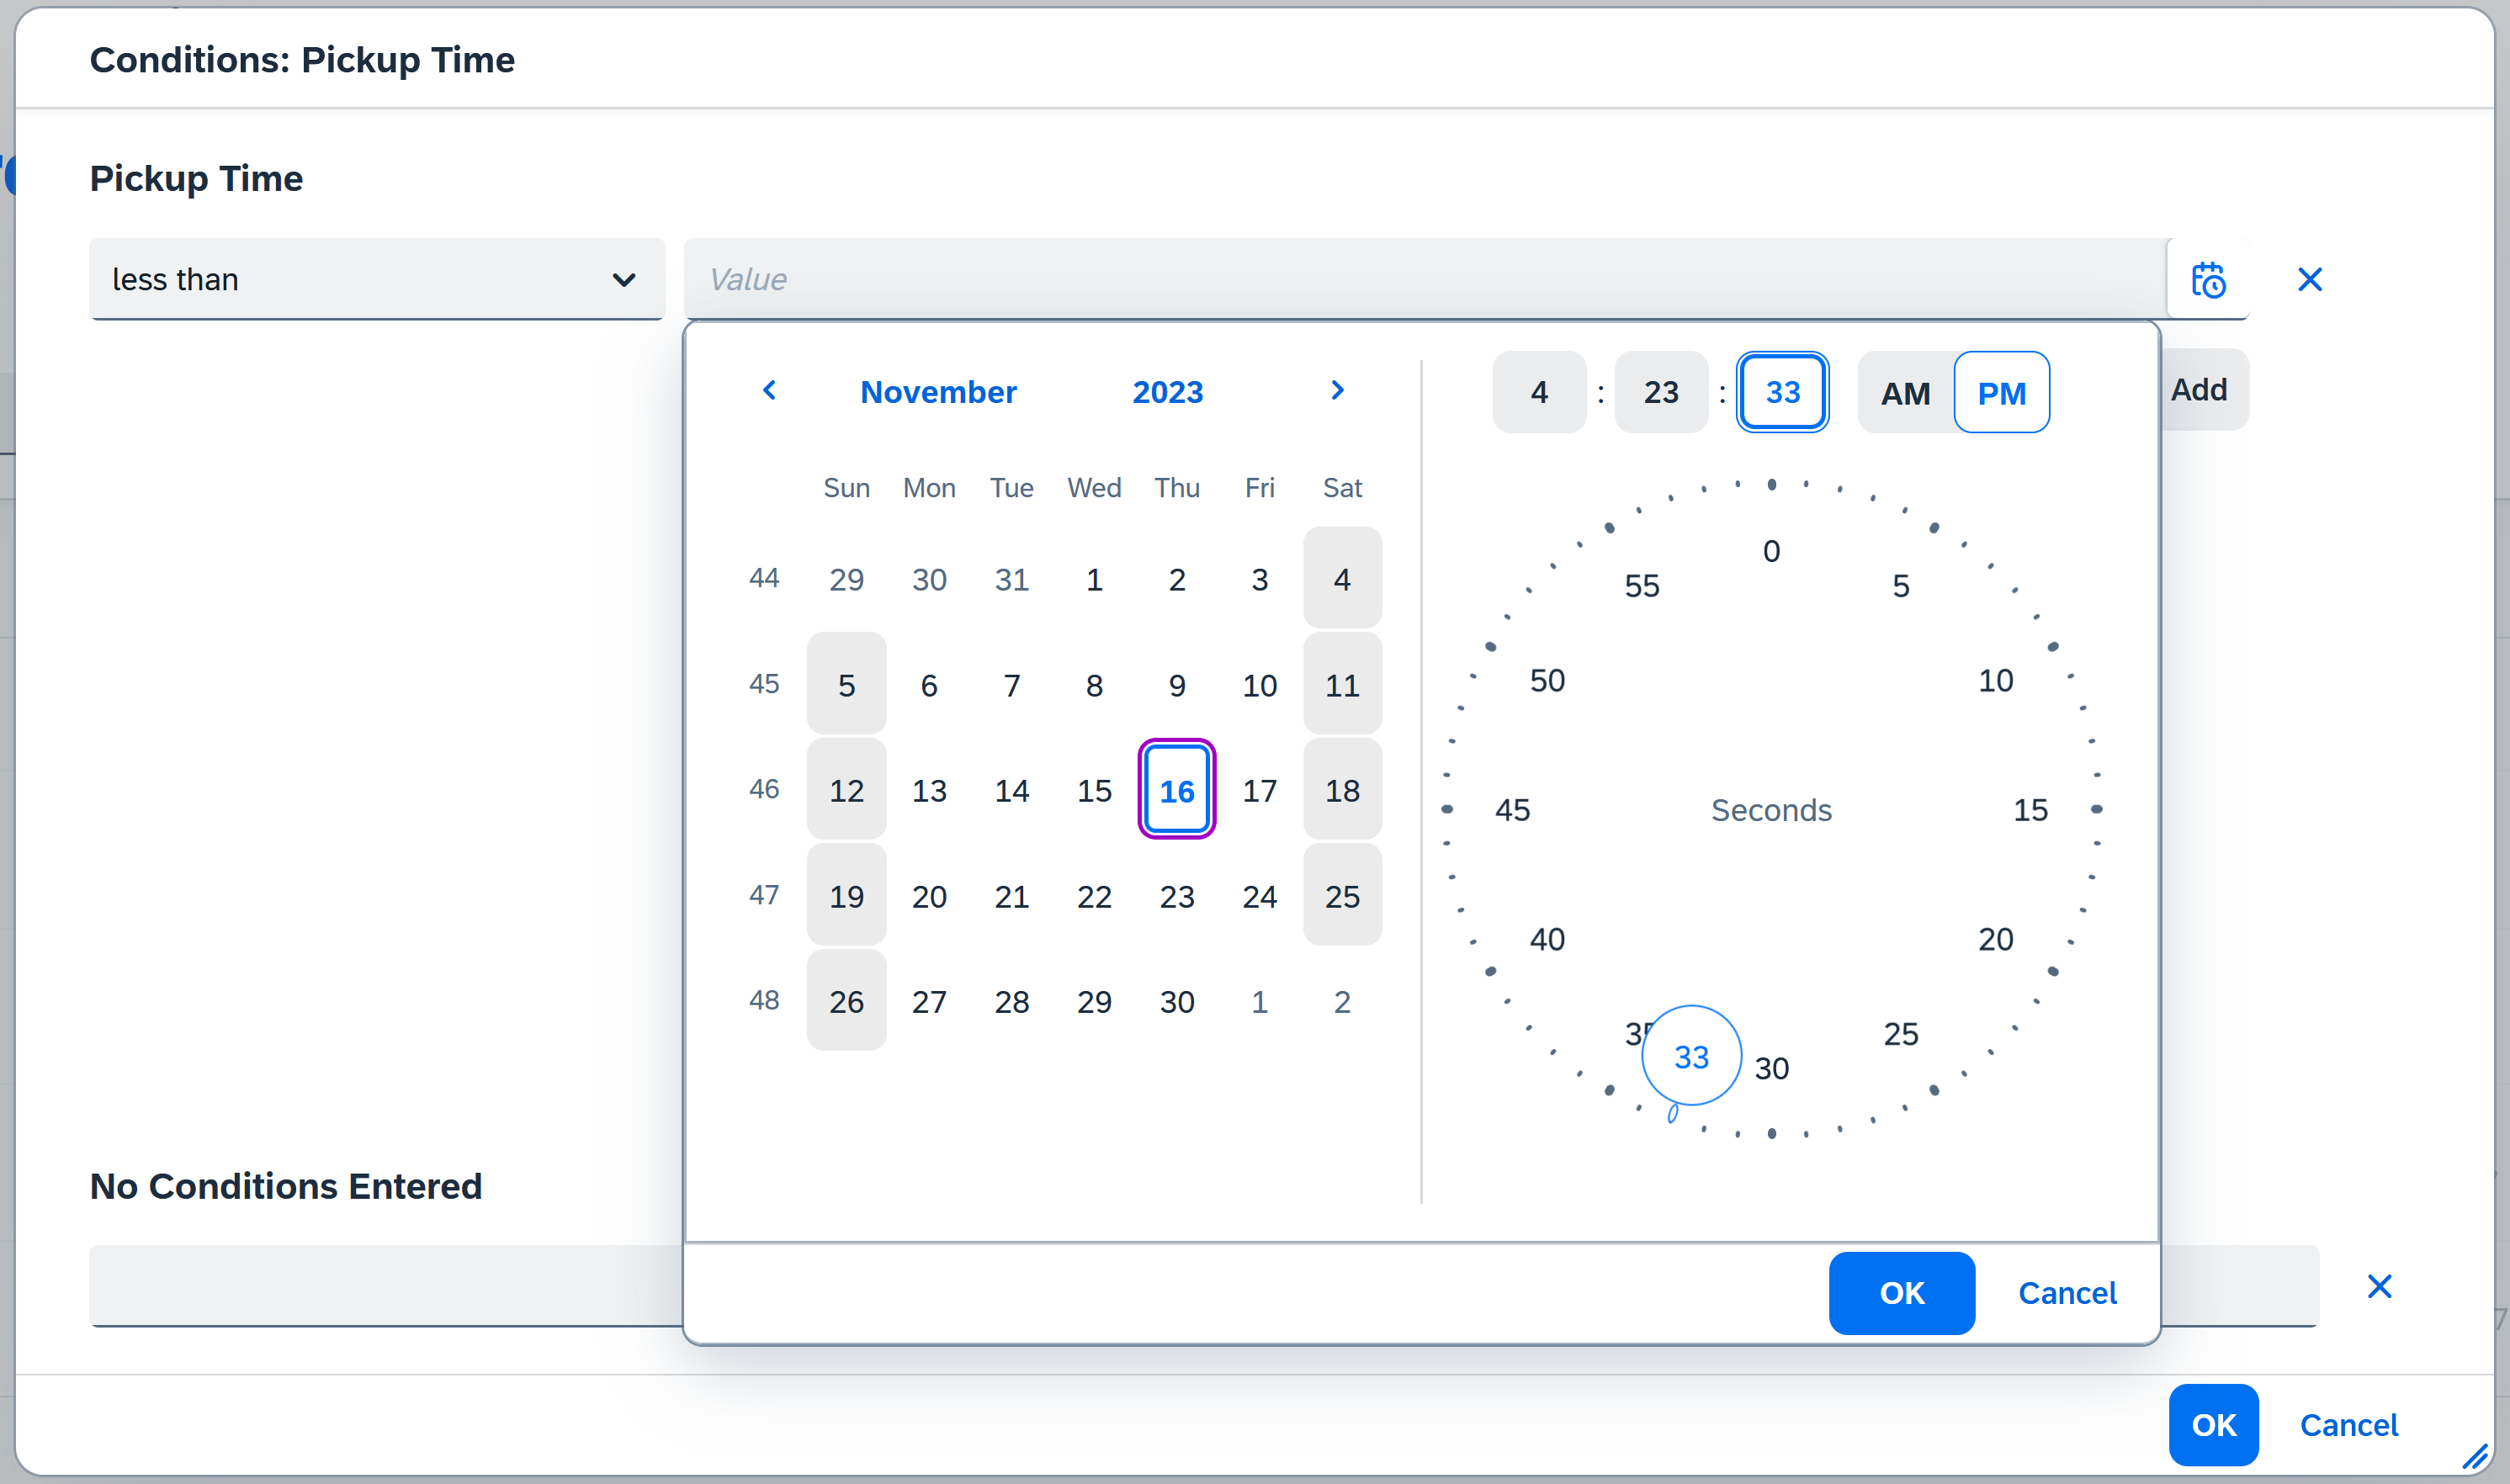
\includegraphics[width=0.45\linewidth]{images/user_doc/myPack/timeFilter-Usage2.png}}
    \caption{Time Filter Dialog - Adjust Filters}
\end{figure}


\begin{figure}[H]
		\centering
	\subcaptionbox{While Adjusting the Filter}{
		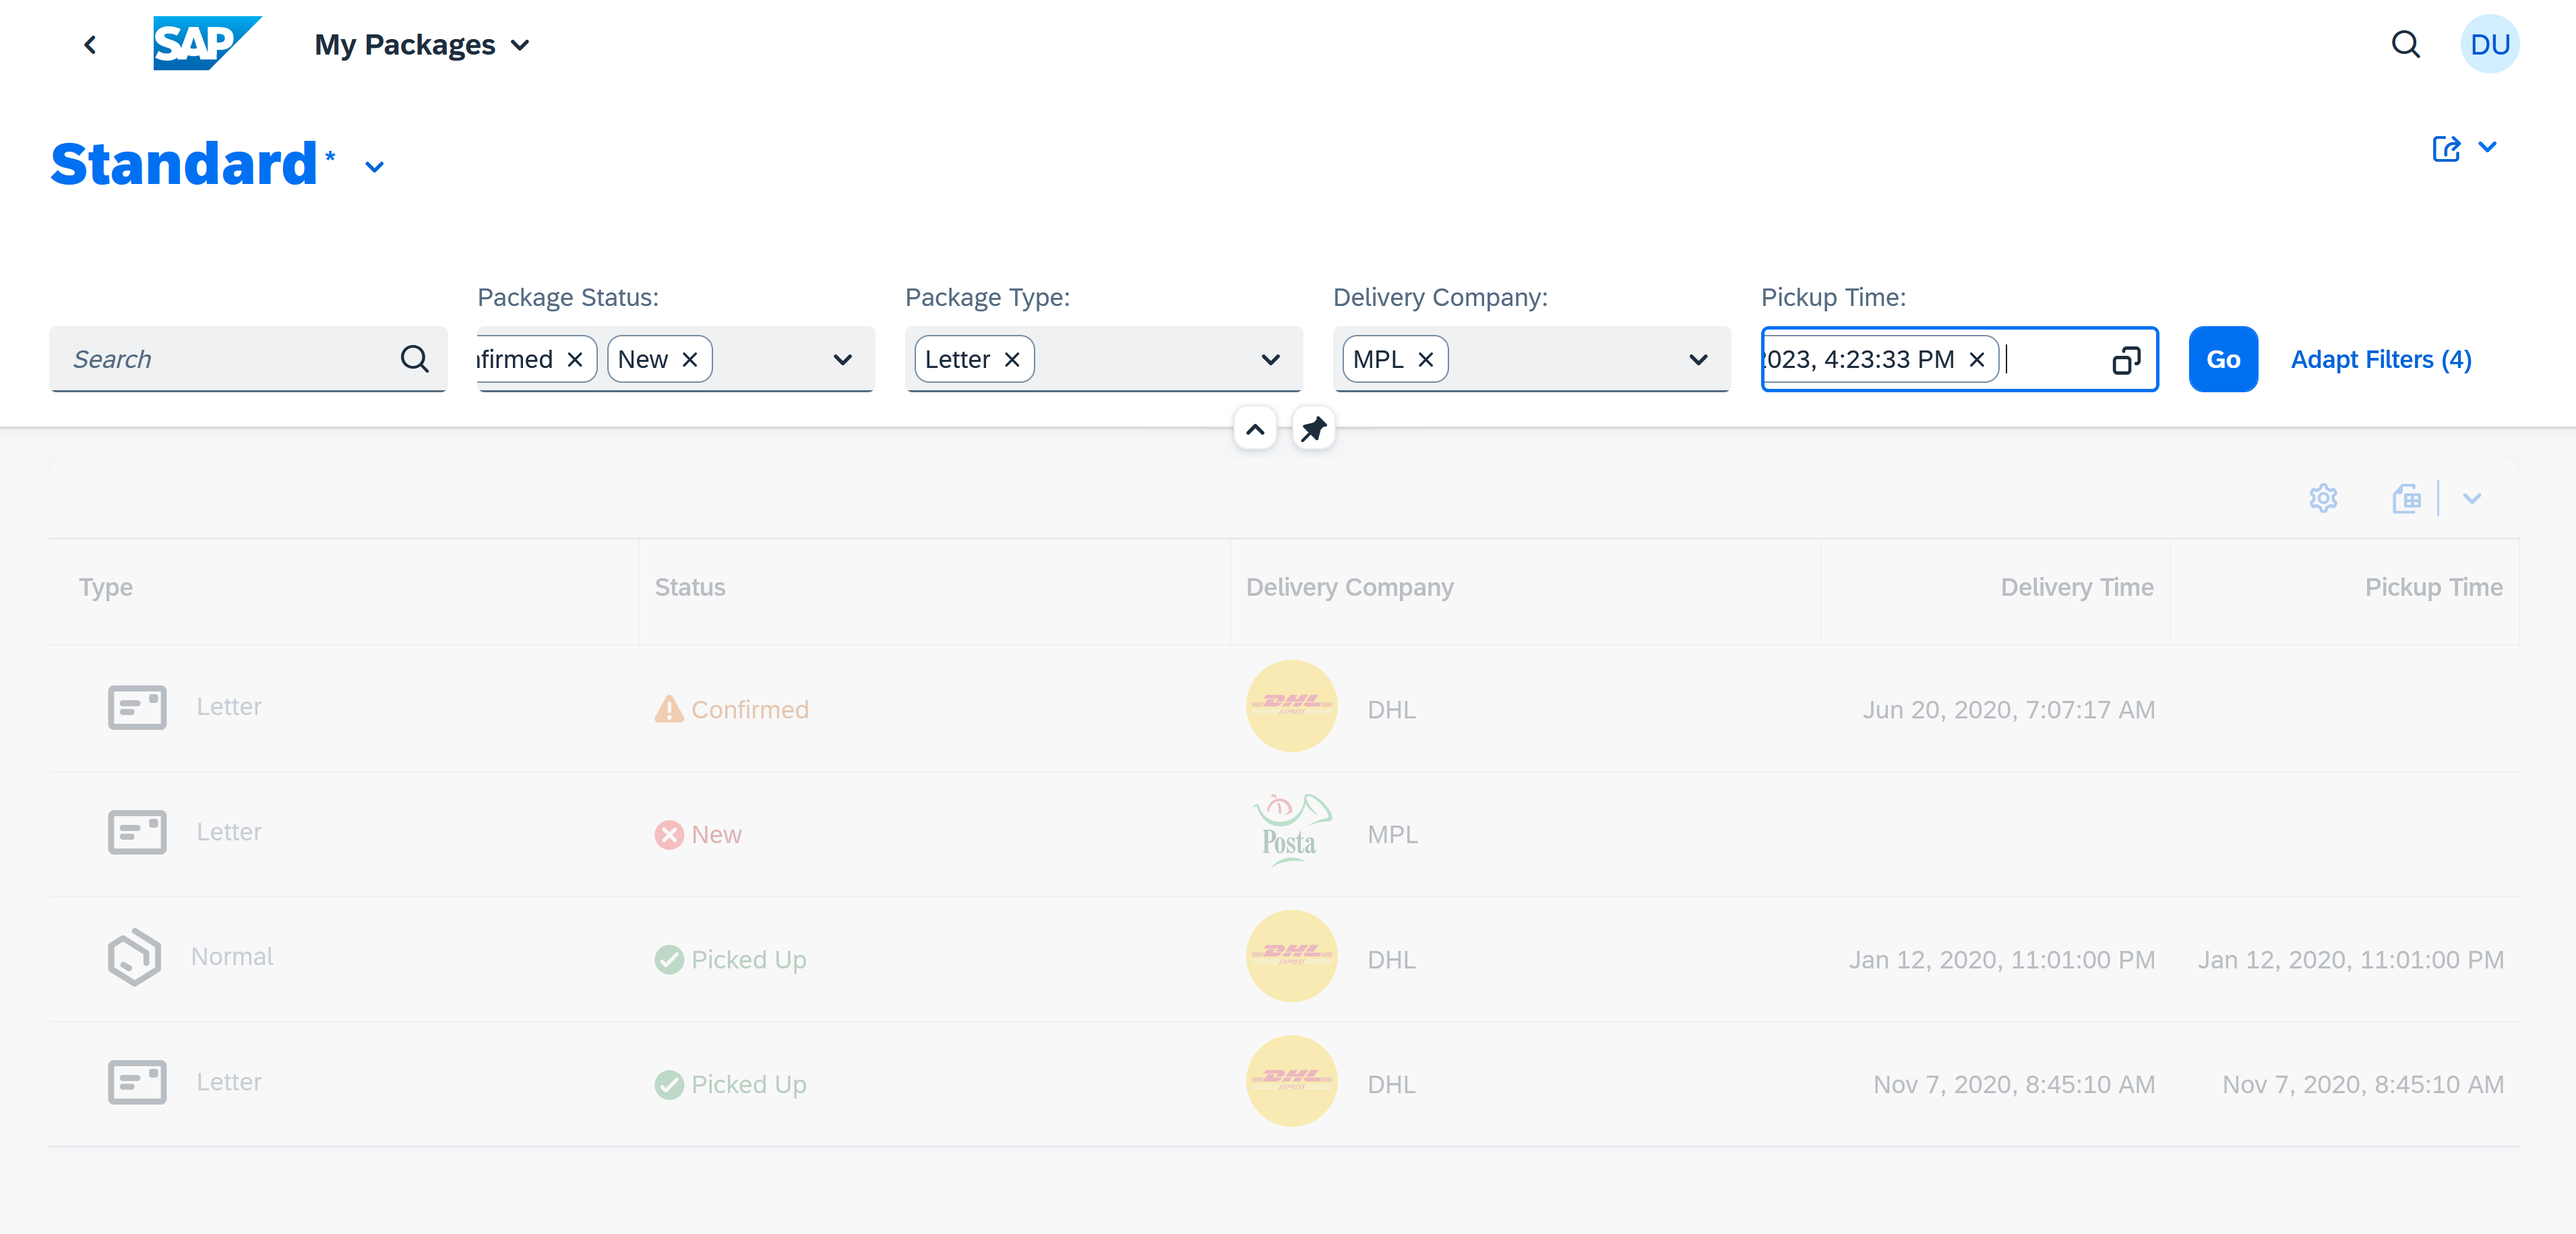
\includegraphics[width=0.45\linewidth]{images/user_doc/myPack/filterAdaptionScreen.png}}
	\hspace{5pt}
	\subcaptionbox{Clicked "Go"}{
		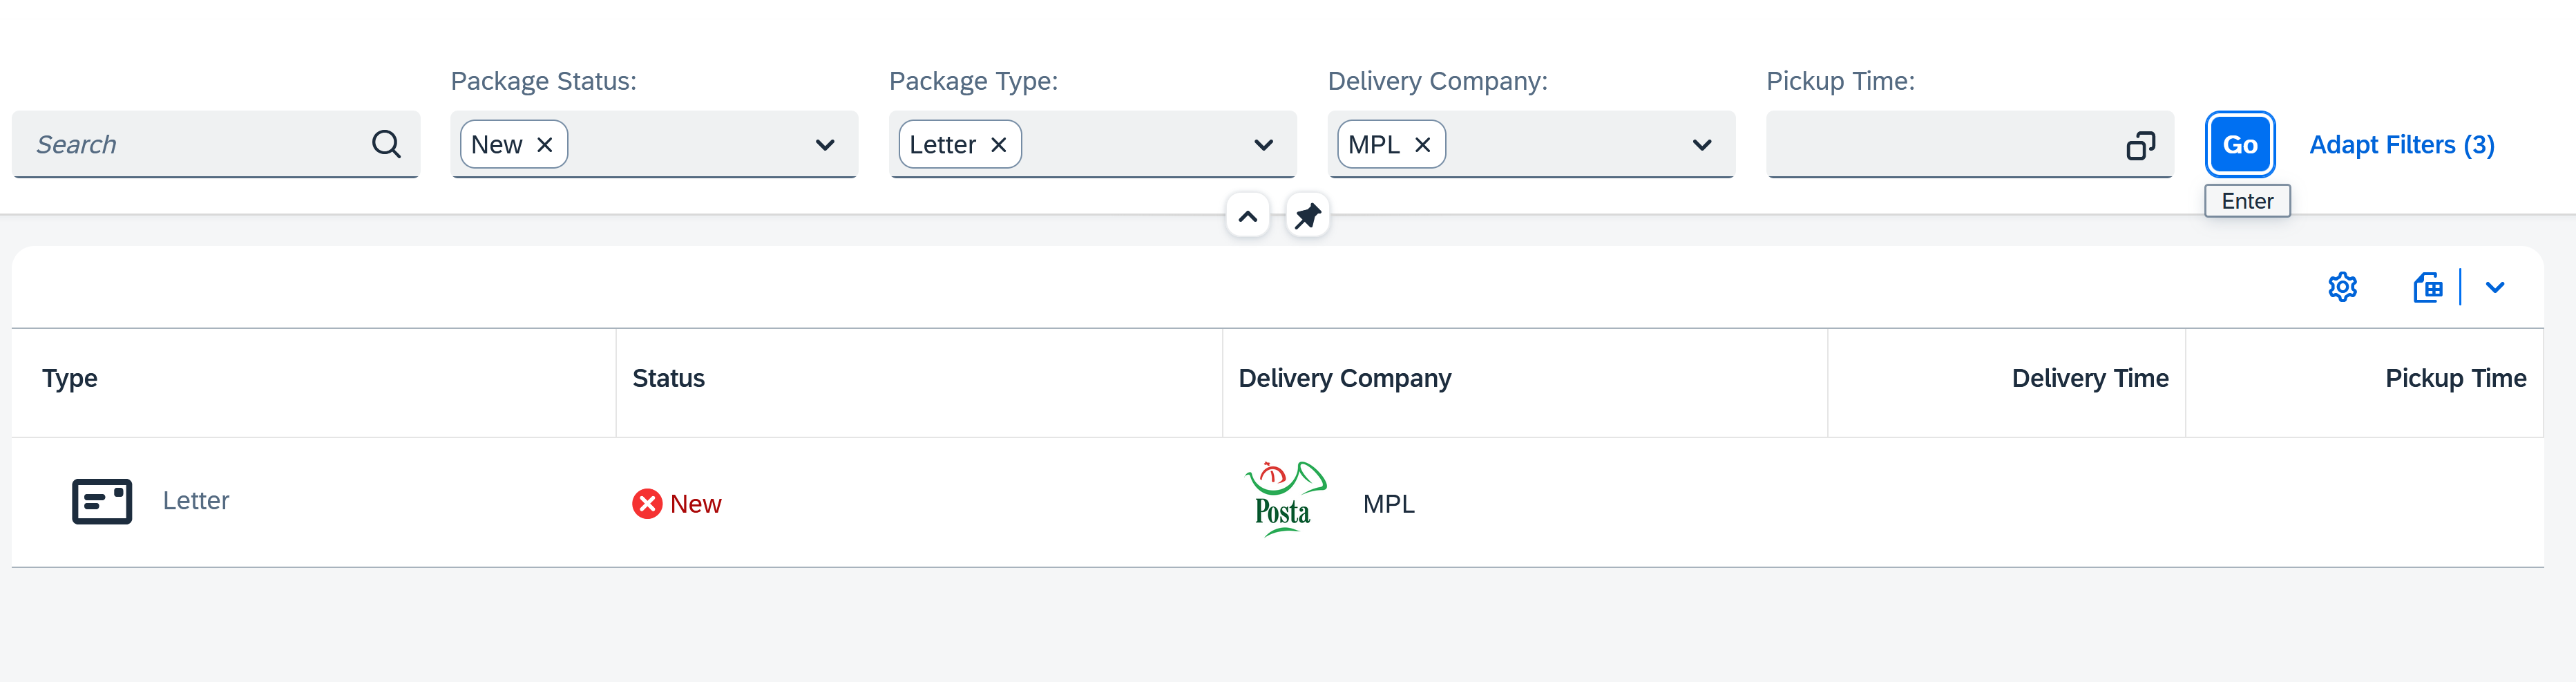
\includegraphics[width=0.45\linewidth]{images/user_doc/myPack/FilterDoneScreen.png}}
    \caption{My Package Home Screen - Adjust Filters}
\end{figure}

\begin{figure}[H]
	\centering
	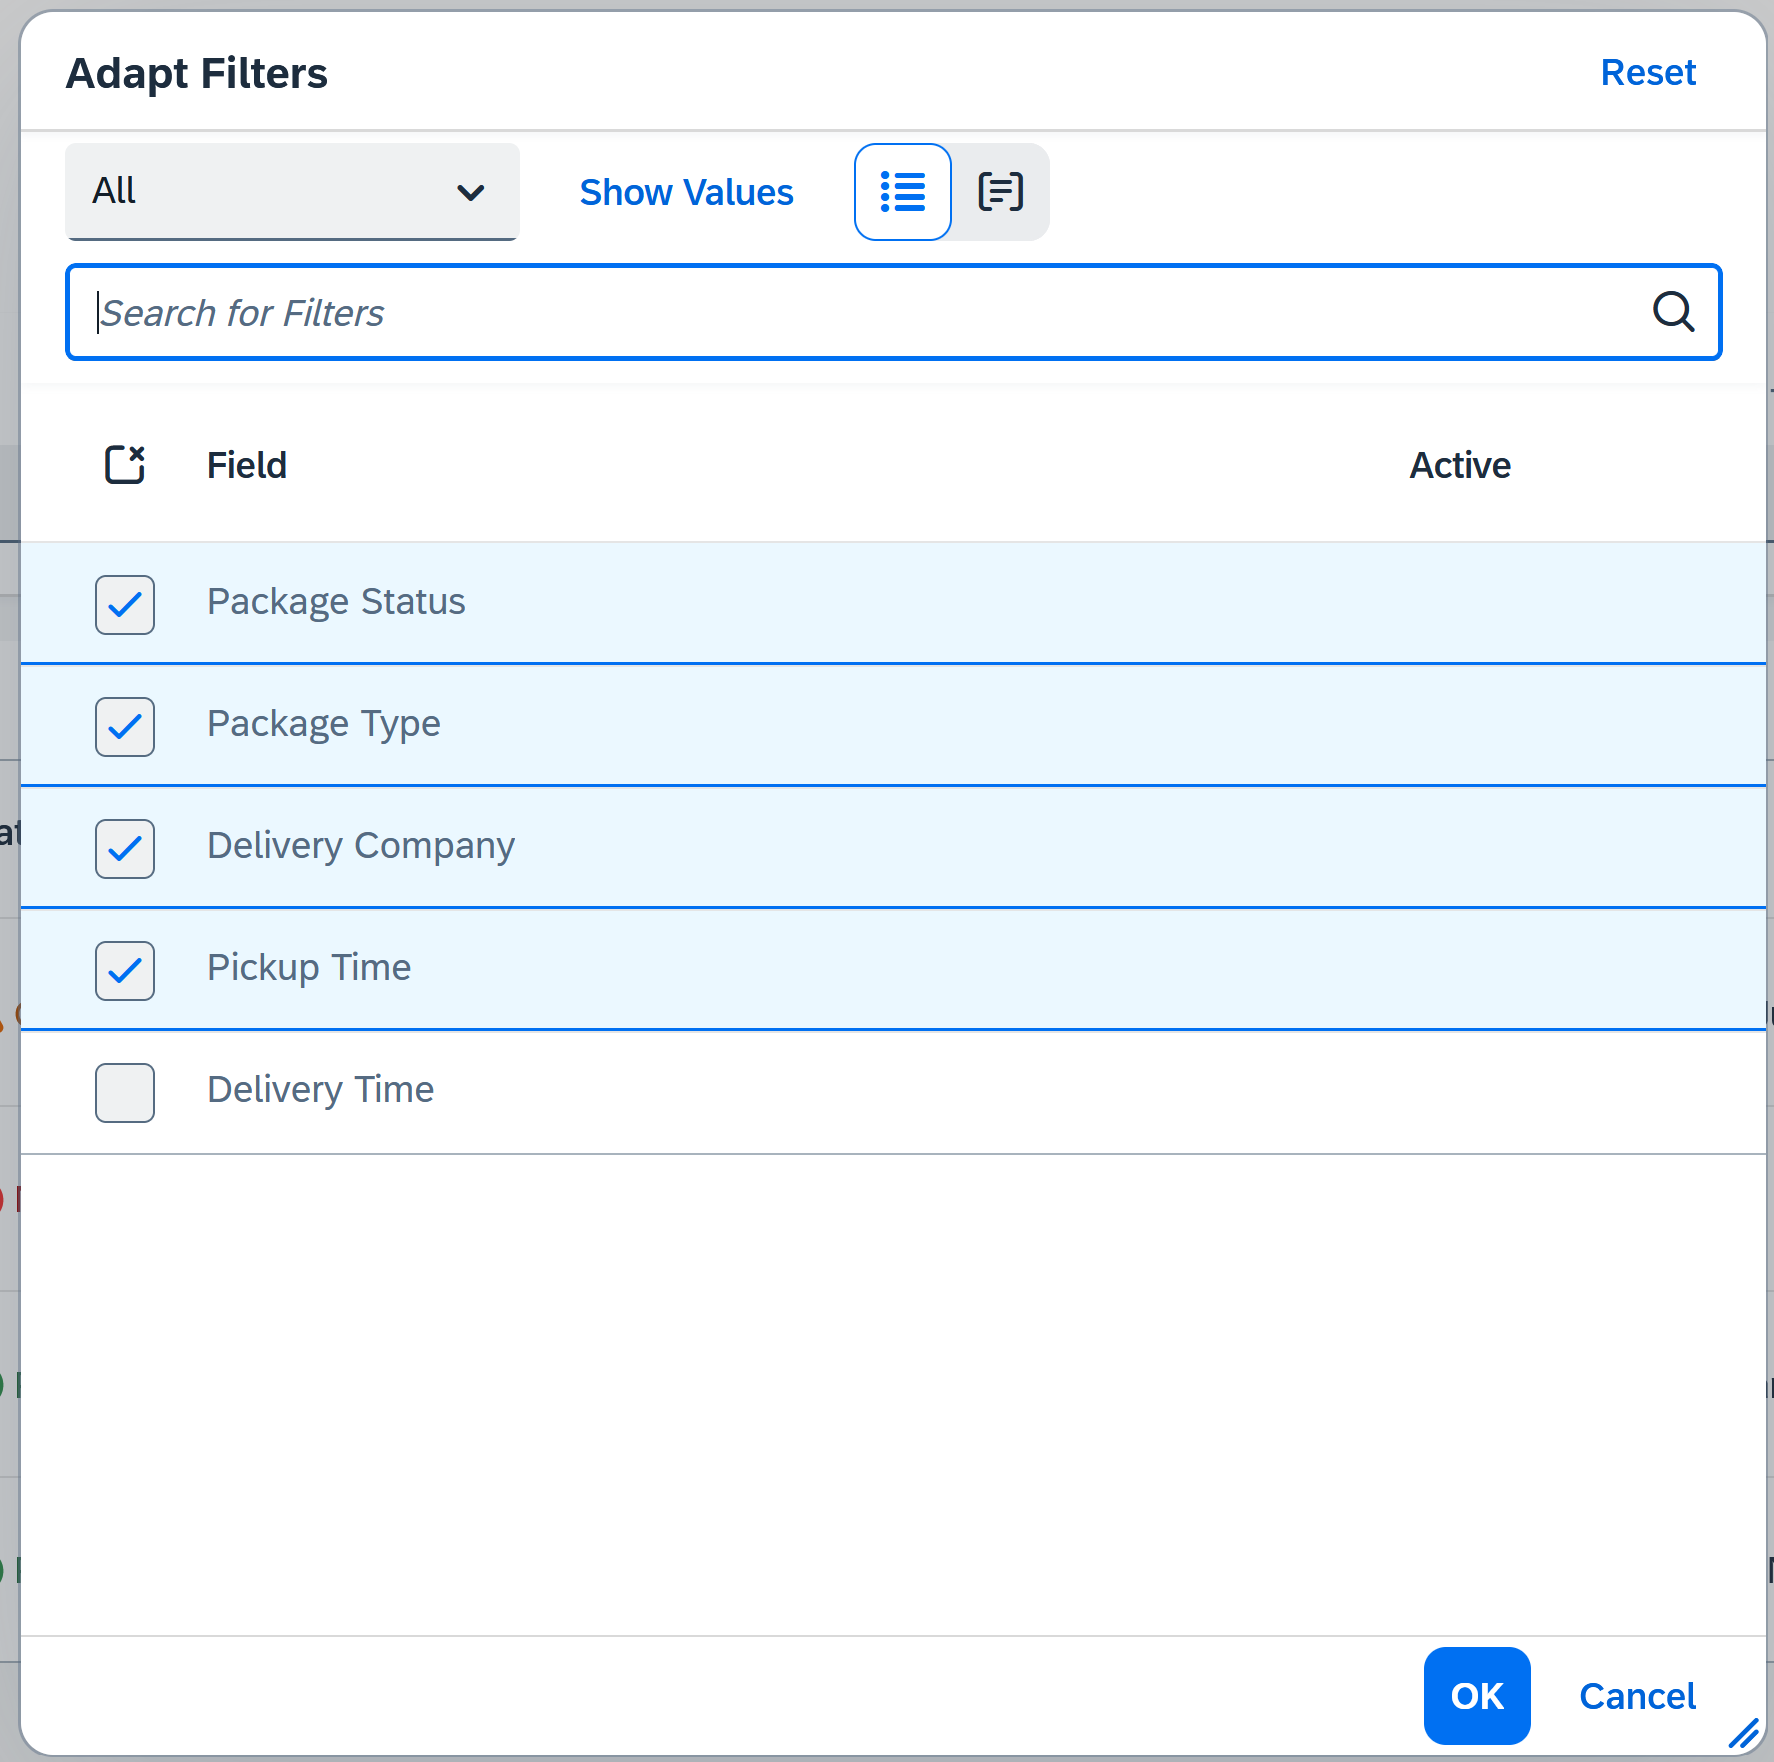
\includegraphics[height=200pt]{images/user_doc/myPack/MoreFIlterOption.png}
	\caption{My Package Filter Adaption Dialog - More Filters}
	\label{fig:mpMOreFilterAdaption}
\end{figure}
% ----------------------- Package Pickup ----------------------------
% 
%  ---------------------------------------------------------------

\subsection{Package Pickup}
The \textbf{Package Pickup} application is used to pick up any confirmed parcels (registered at the reception and confirmed with a storage slot) of the logged in user. One can only see one's own confirmed packages. 

\textbf{Hint}: The application supports only from mobile devices. In case an employee is unable to access his or her mobile at the moment of pickup, he or she shall ask the receptionist to pickup the package for him or her.

\bigskip

\subsubsection{Home Screen - Selection}
As an \textbf{End User}, after clicking at the application tile, is redirected to the "Home Screen". If there exists at least one package to pickup, the home screen shows the list of packages. The list items lists \textbf{the type with icon, the delivery company, the registration time and the location} of the packages. If no package exists to pickup, it shows only the no package info. The package list title shows the total number of packages that can be pickup.

In case there are existing packages, one can select one or multiple packages from the list to pickup. 

In case there are existing packages, one can tick/untick the "Toggle All" selection box to select or deselect the package all at once. 

\begin{figure}[H]
	\centering
	\subcaptionbox{Home Screen with Packages}{
		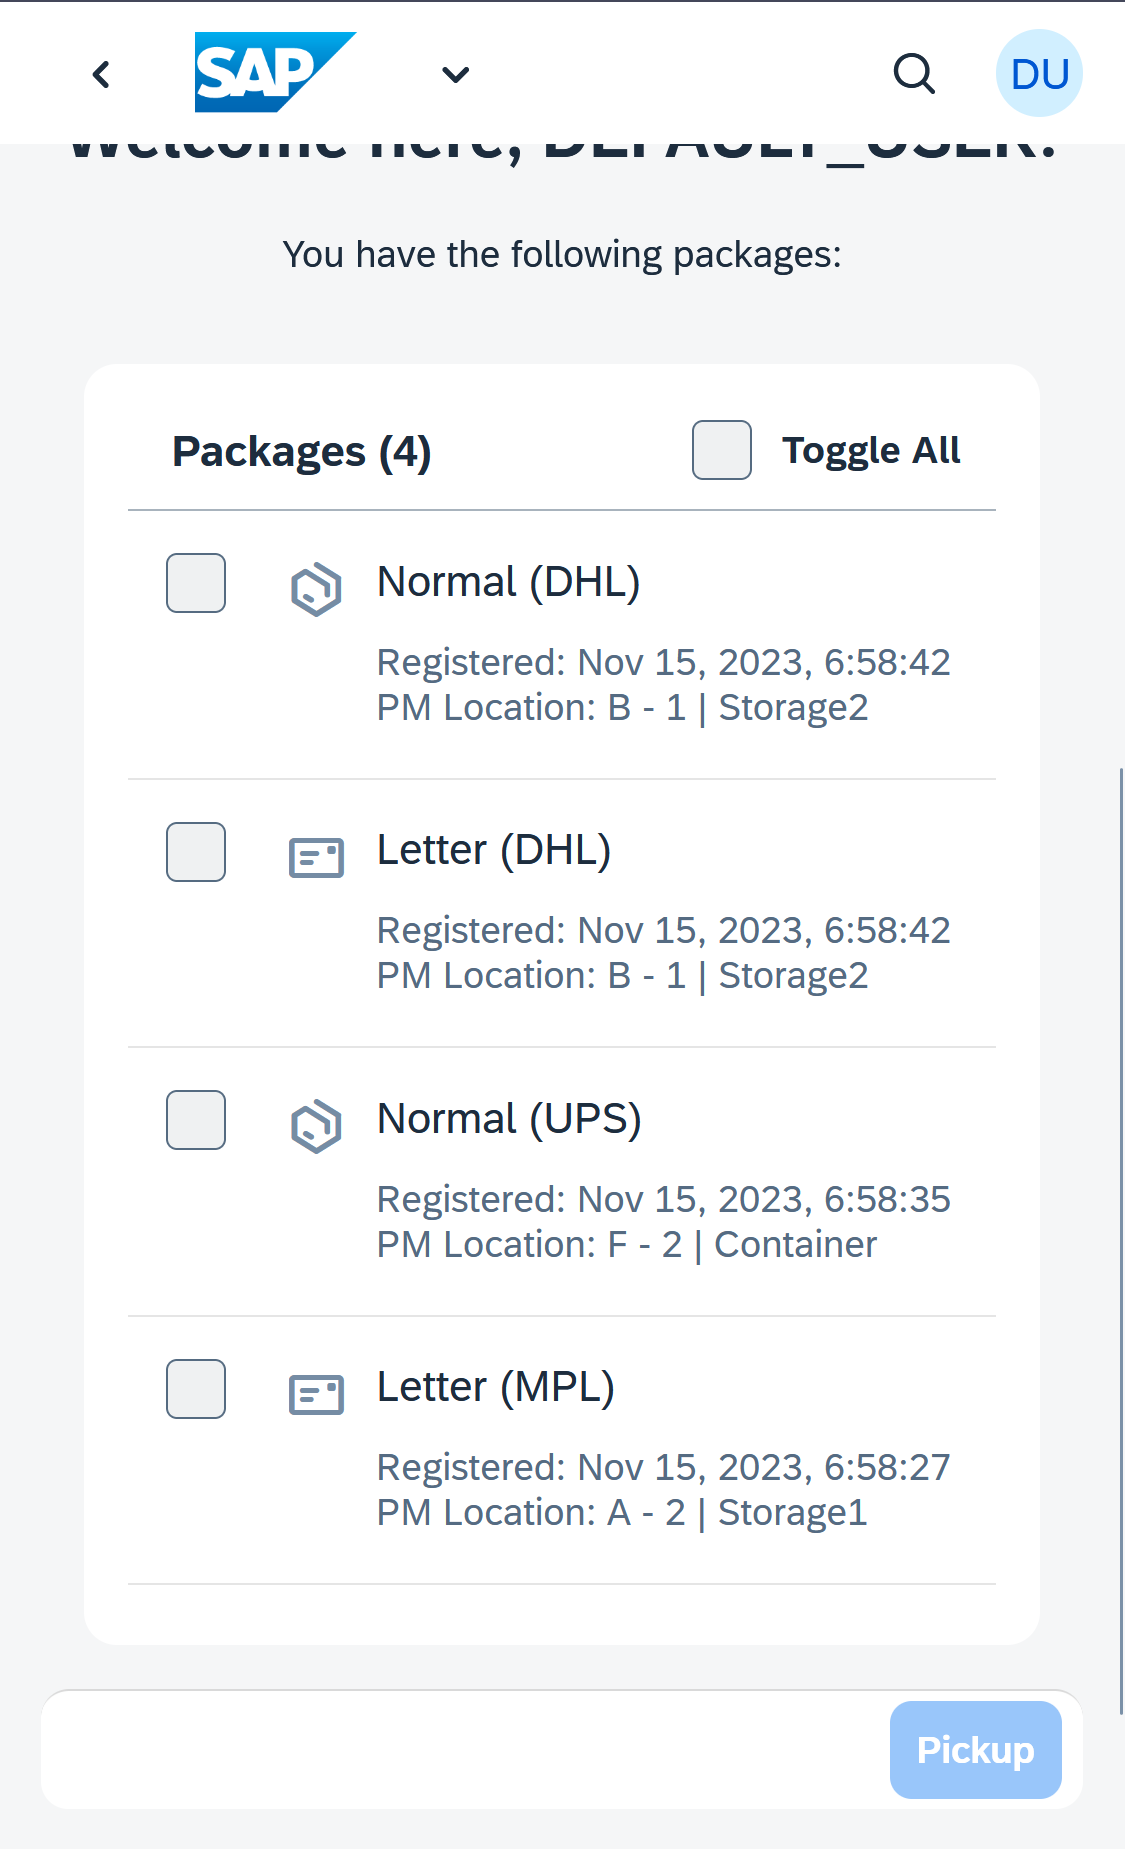
\includegraphics[width=0.45\linewidth]{images/user_doc/pickup/HomeScreenList.png}}
	\hspace{5pt}
	\subcaptionbox{Home Screen without Packages}{
		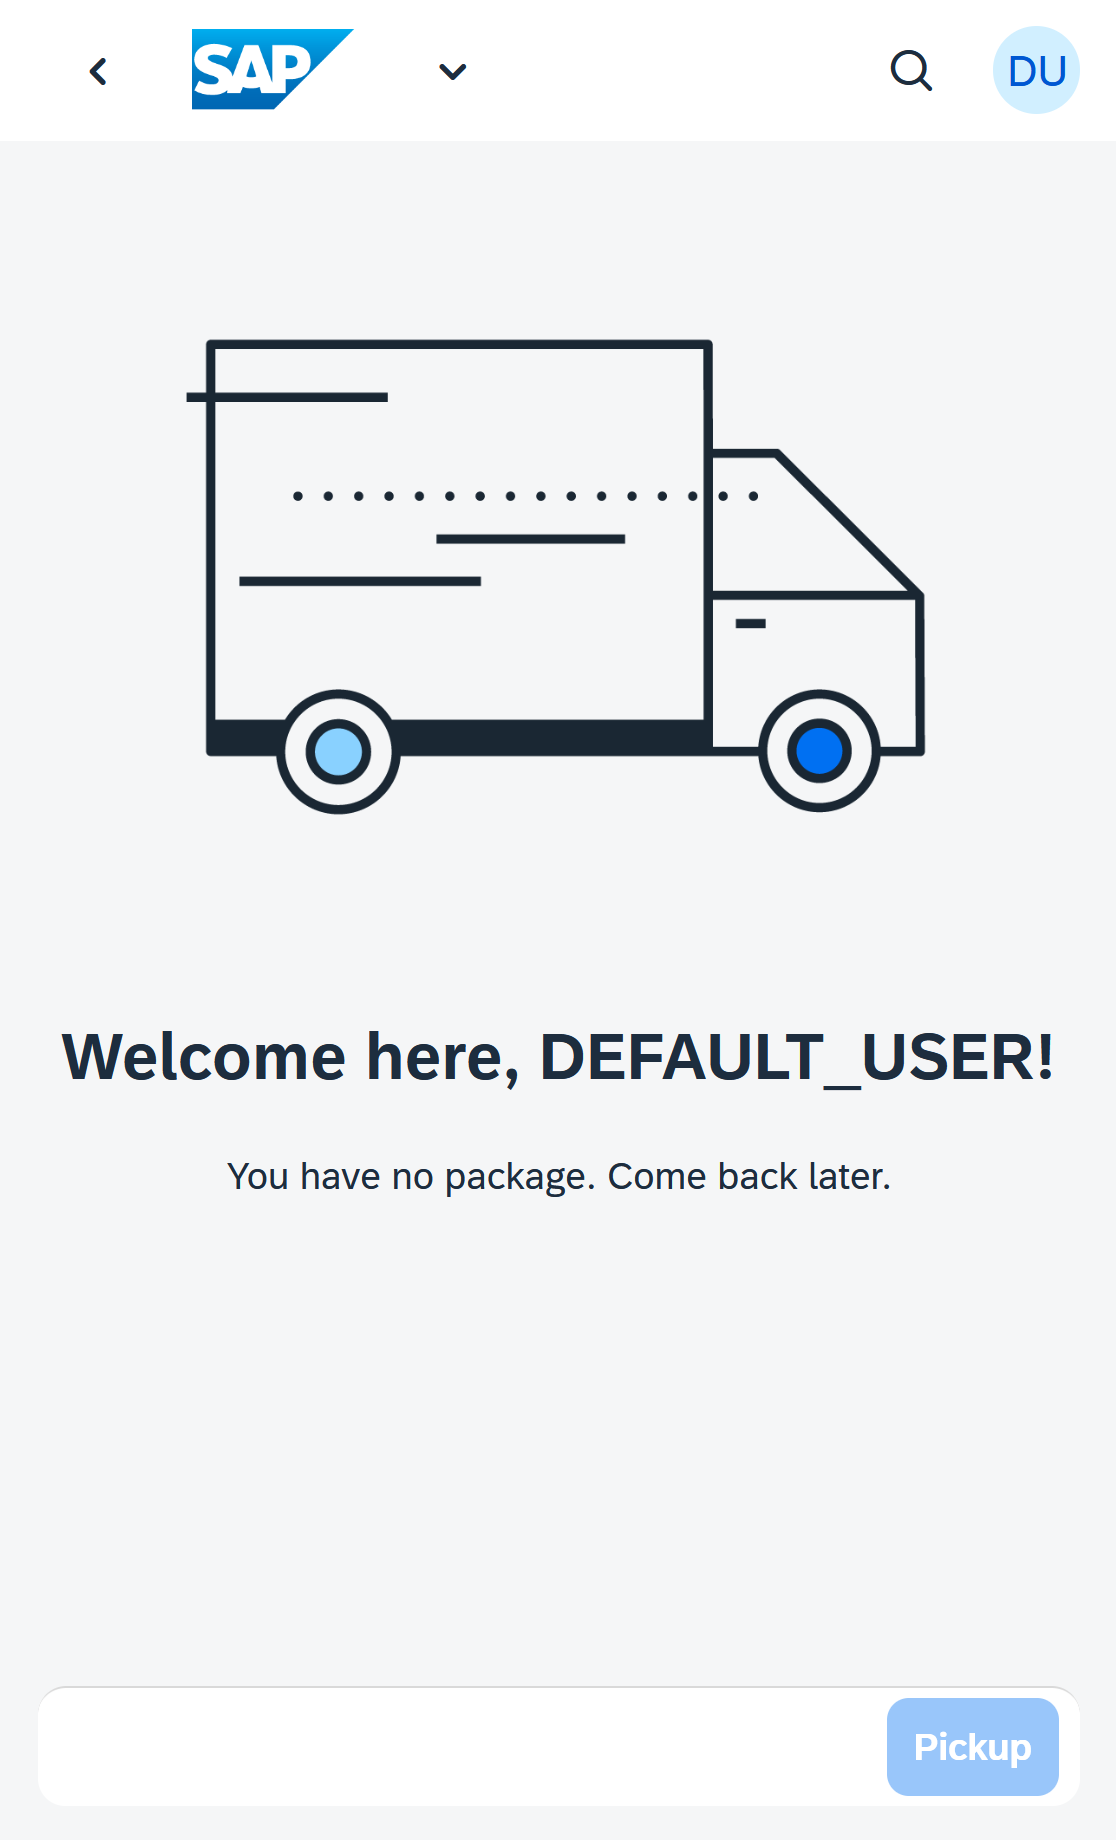
\includegraphics[width=0.45\linewidth]{images/user_doc/pickup/HomeScreenNoPackage.png}}
	\caption{Pickup Home Screen - Package Existence Guide}
	\label{fig:PickupHomeScreen-1}
\end{figure}

\begin{figure}[H]
	\centering
	\subcaptionbox{Home Screen Single Selection}{
		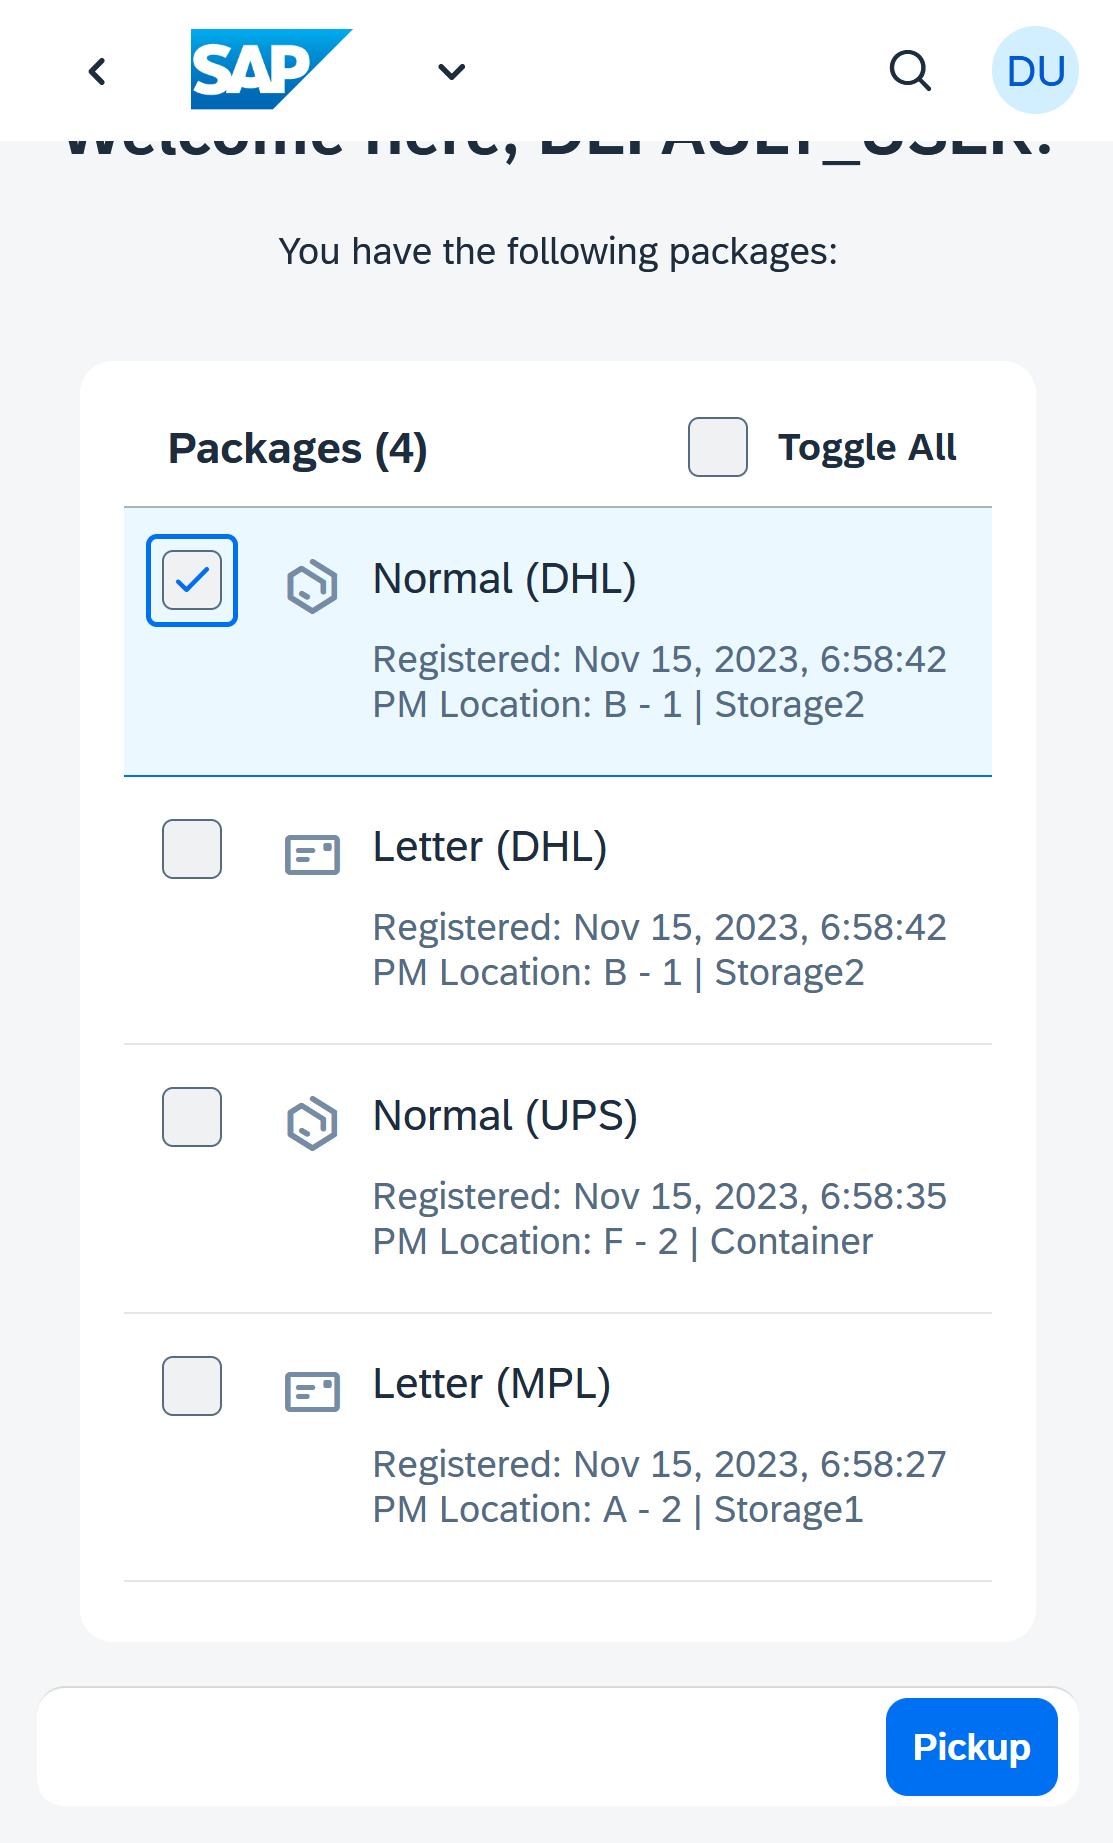
\includegraphics[width=0.45\linewidth]{images/user_doc/pickup/HomeScreenSelectOne.png}}
	\hspace{5pt}
	\subcaptionbox{Home Screen Multiple Selection}{
		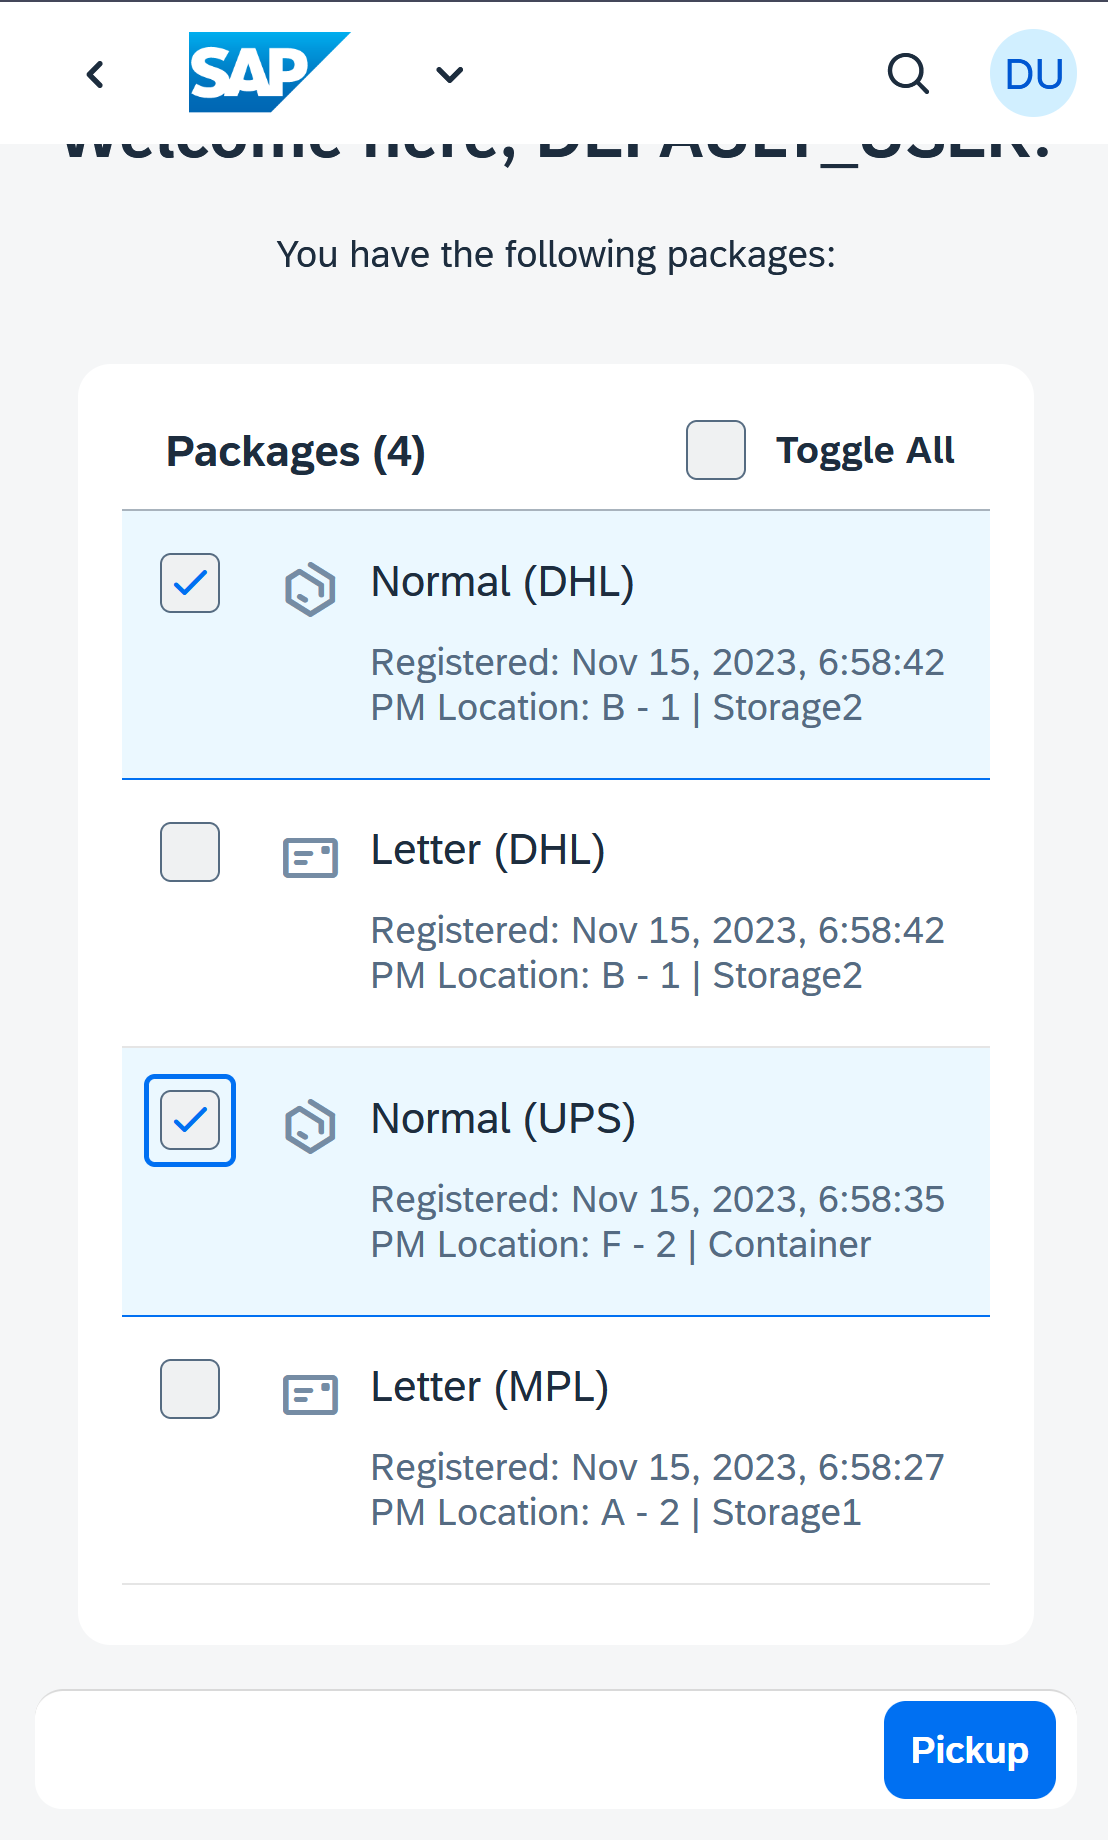
\includegraphics[width=0.45\linewidth]{images/user_doc/pickup/HomeScreenMultiSelect.png}}

    \subcaptionbox{Home Screen Select All}{
		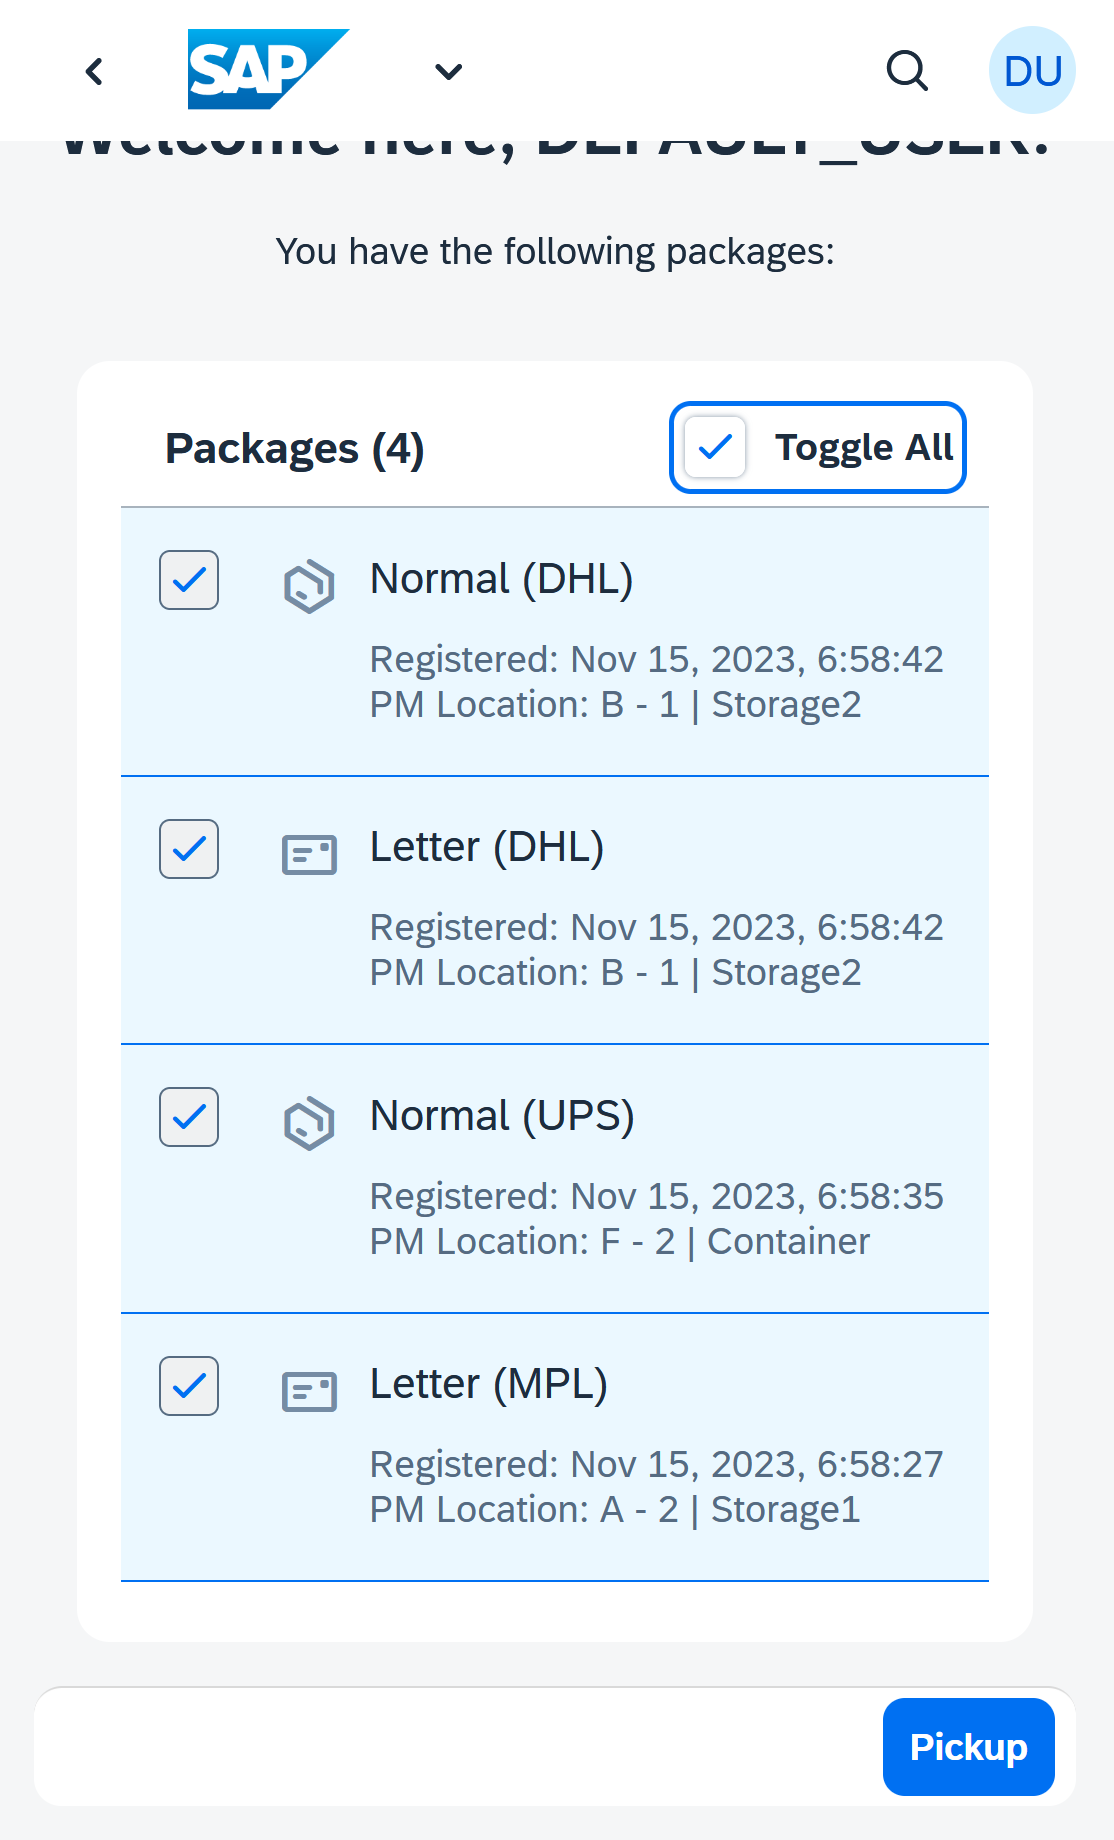
\includegraphics[width=0.45\linewidth]{images/user_doc/pickup/HomeScreenToggleAll.png}}
	\hspace{5pt}
	\subcaptionbox{Home Screen Deselect All}{
		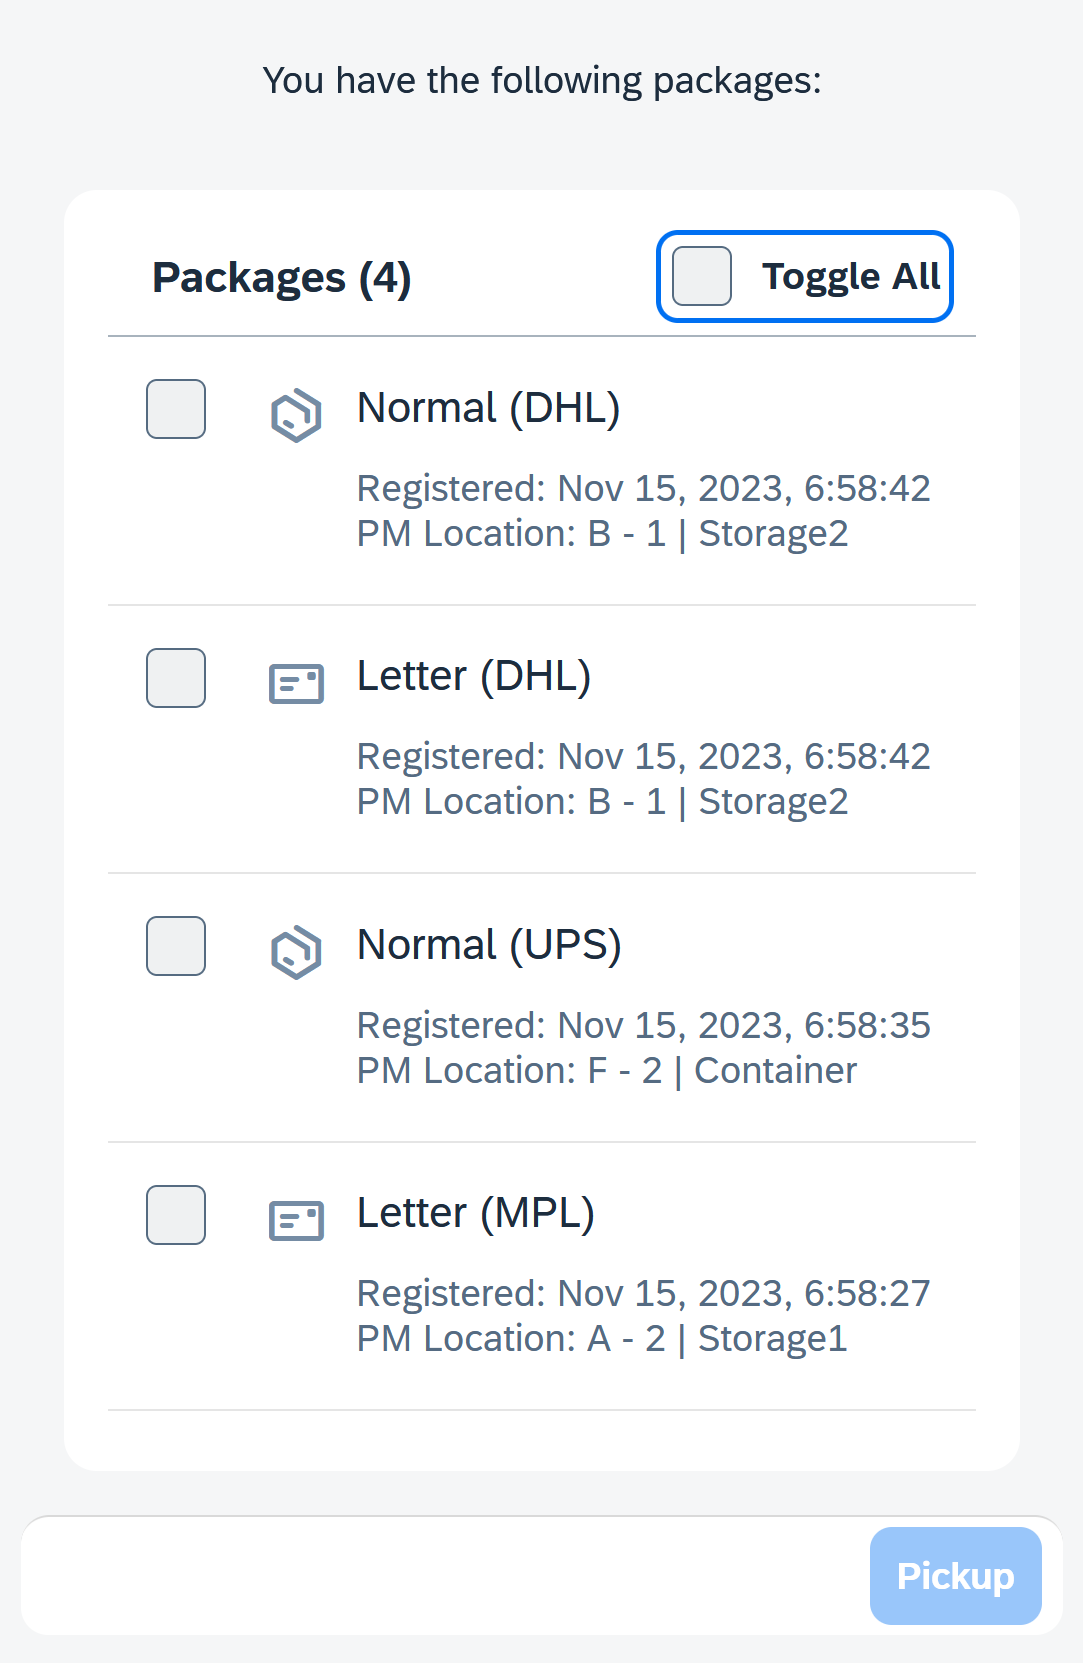
\includegraphics[width=0.45\linewidth]{images/user_doc/pickup/HomeScreenDeToggleAll.png}}
	\caption{Pickup Home Screen - Package Selection Guide}
	\label{fig:PickupHomeScreen-1}
\end{figure}


% \begin{figure}[H]
% 	\centering
% 	\subcaptionbox{Home Screen Single Selection}{
% 		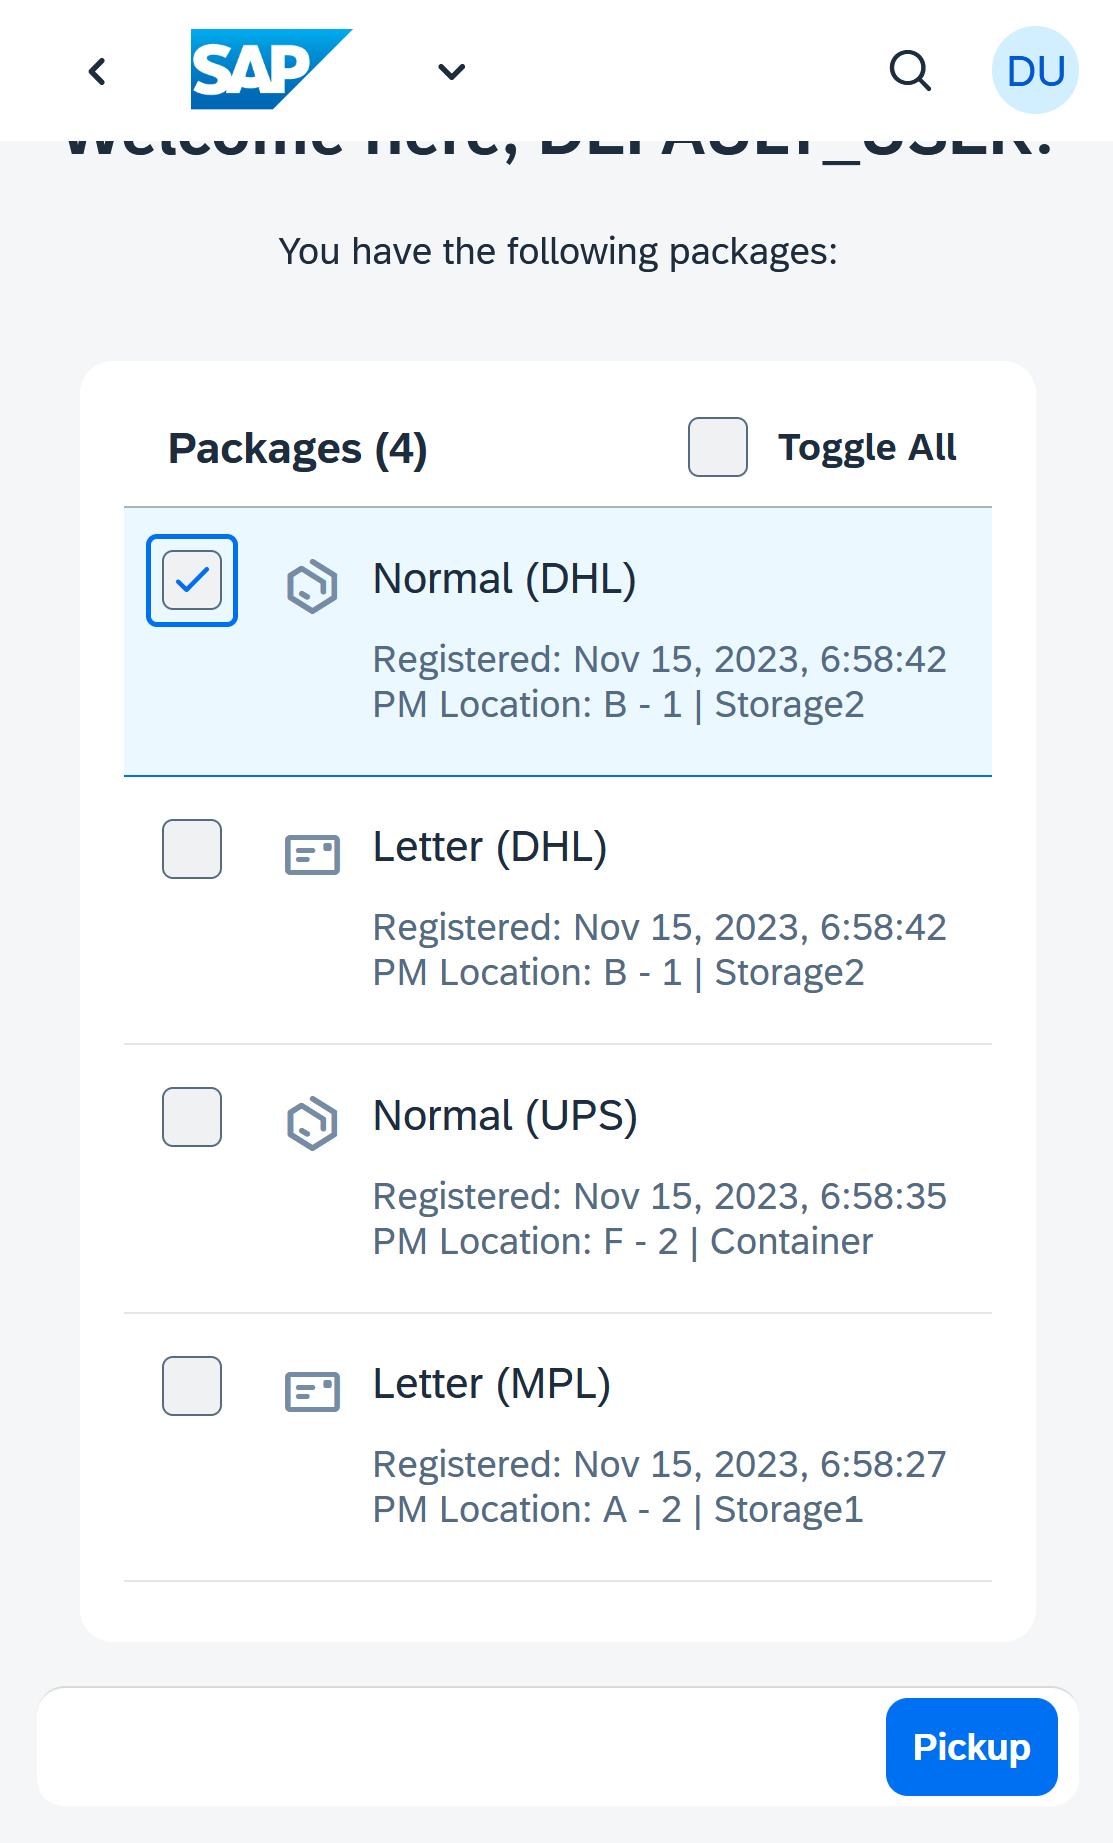
\includegraphics[height=260pt]{images/user_doc/pickup/HomeScreenSelectOne.png}}
% 	\hspace{5pt}
% 	\subcaptionbox{Home Screen Multiple Selection}{
% 		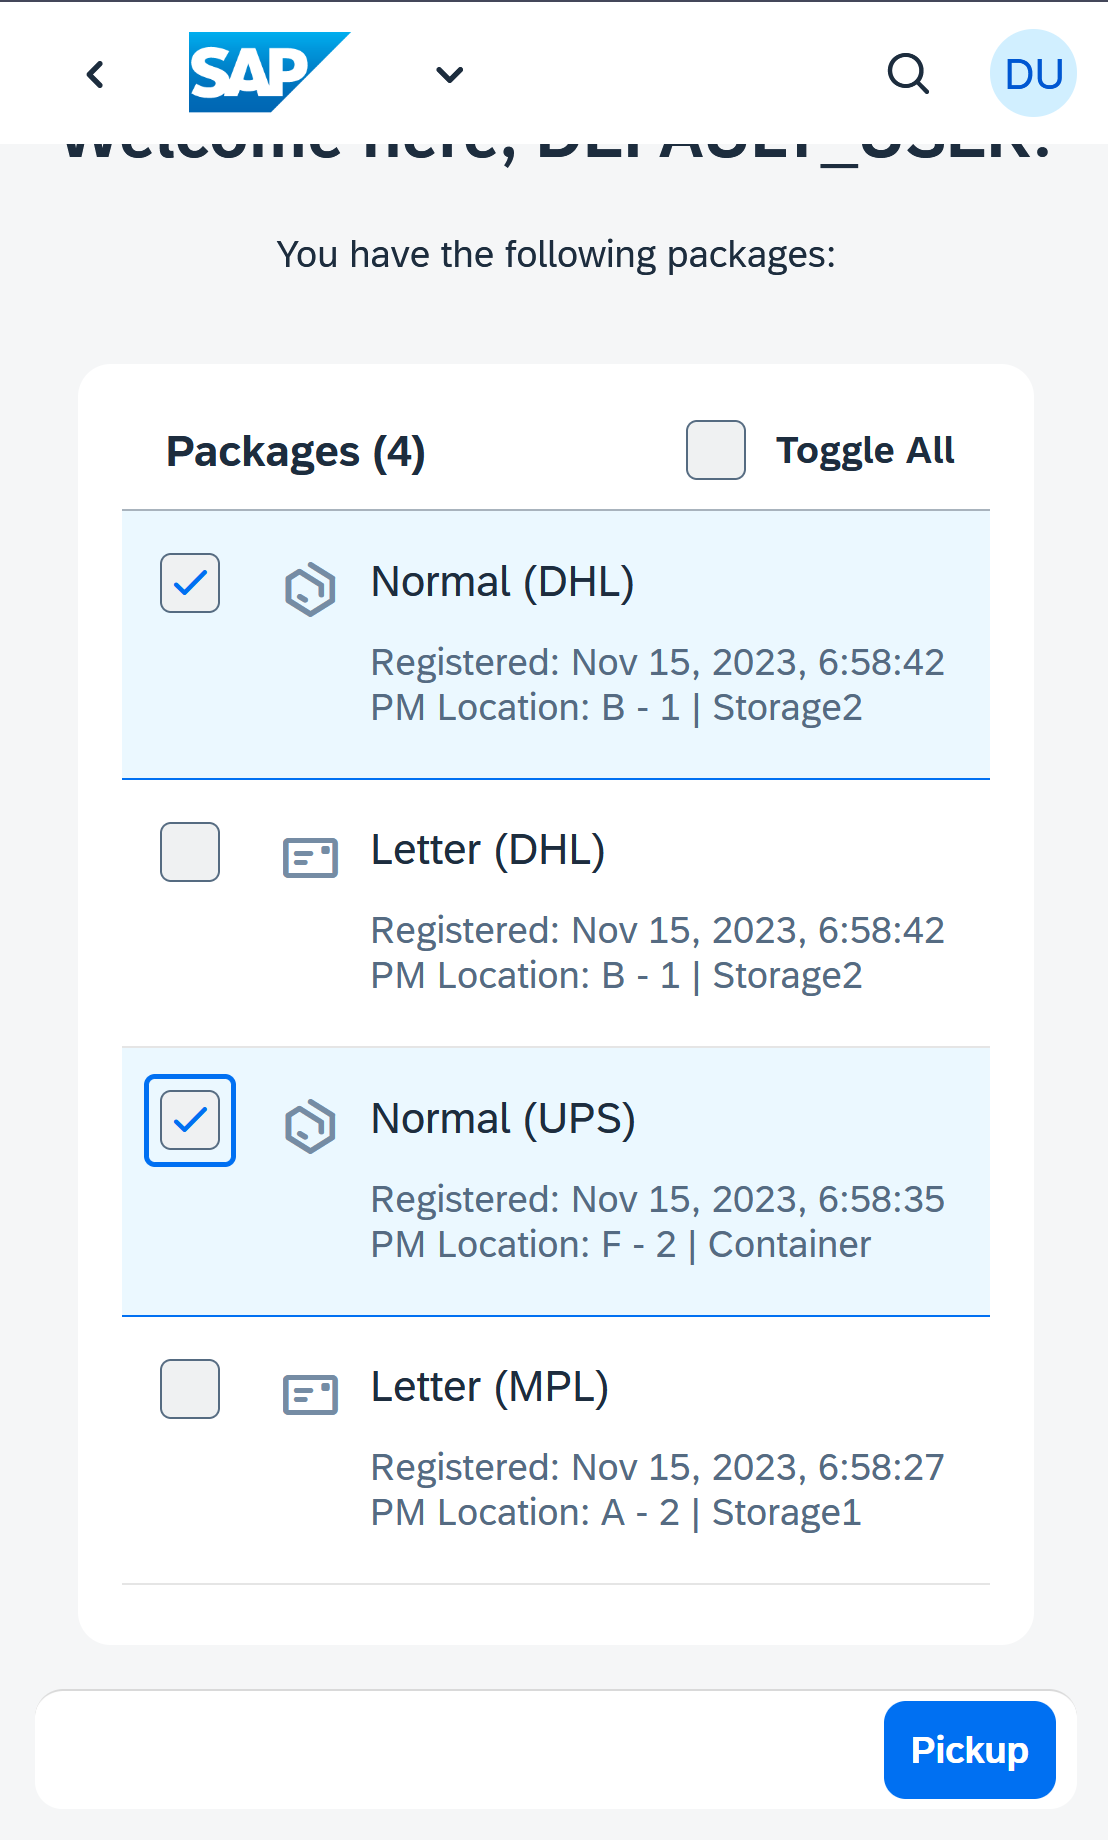
\includegraphics[height=260pt]{images/user_doc/pickup/HomeScreenMultiSelect.png}}
% 	\caption{Pickup Home Screen - Selection Guide}
% 	\label{fig:PickupHomeScreen-2}
% \end{figure}

% \begin{figure}[H]
% 	\centering
% 	\subcaptionbox{Home Screen Select All}{
% 		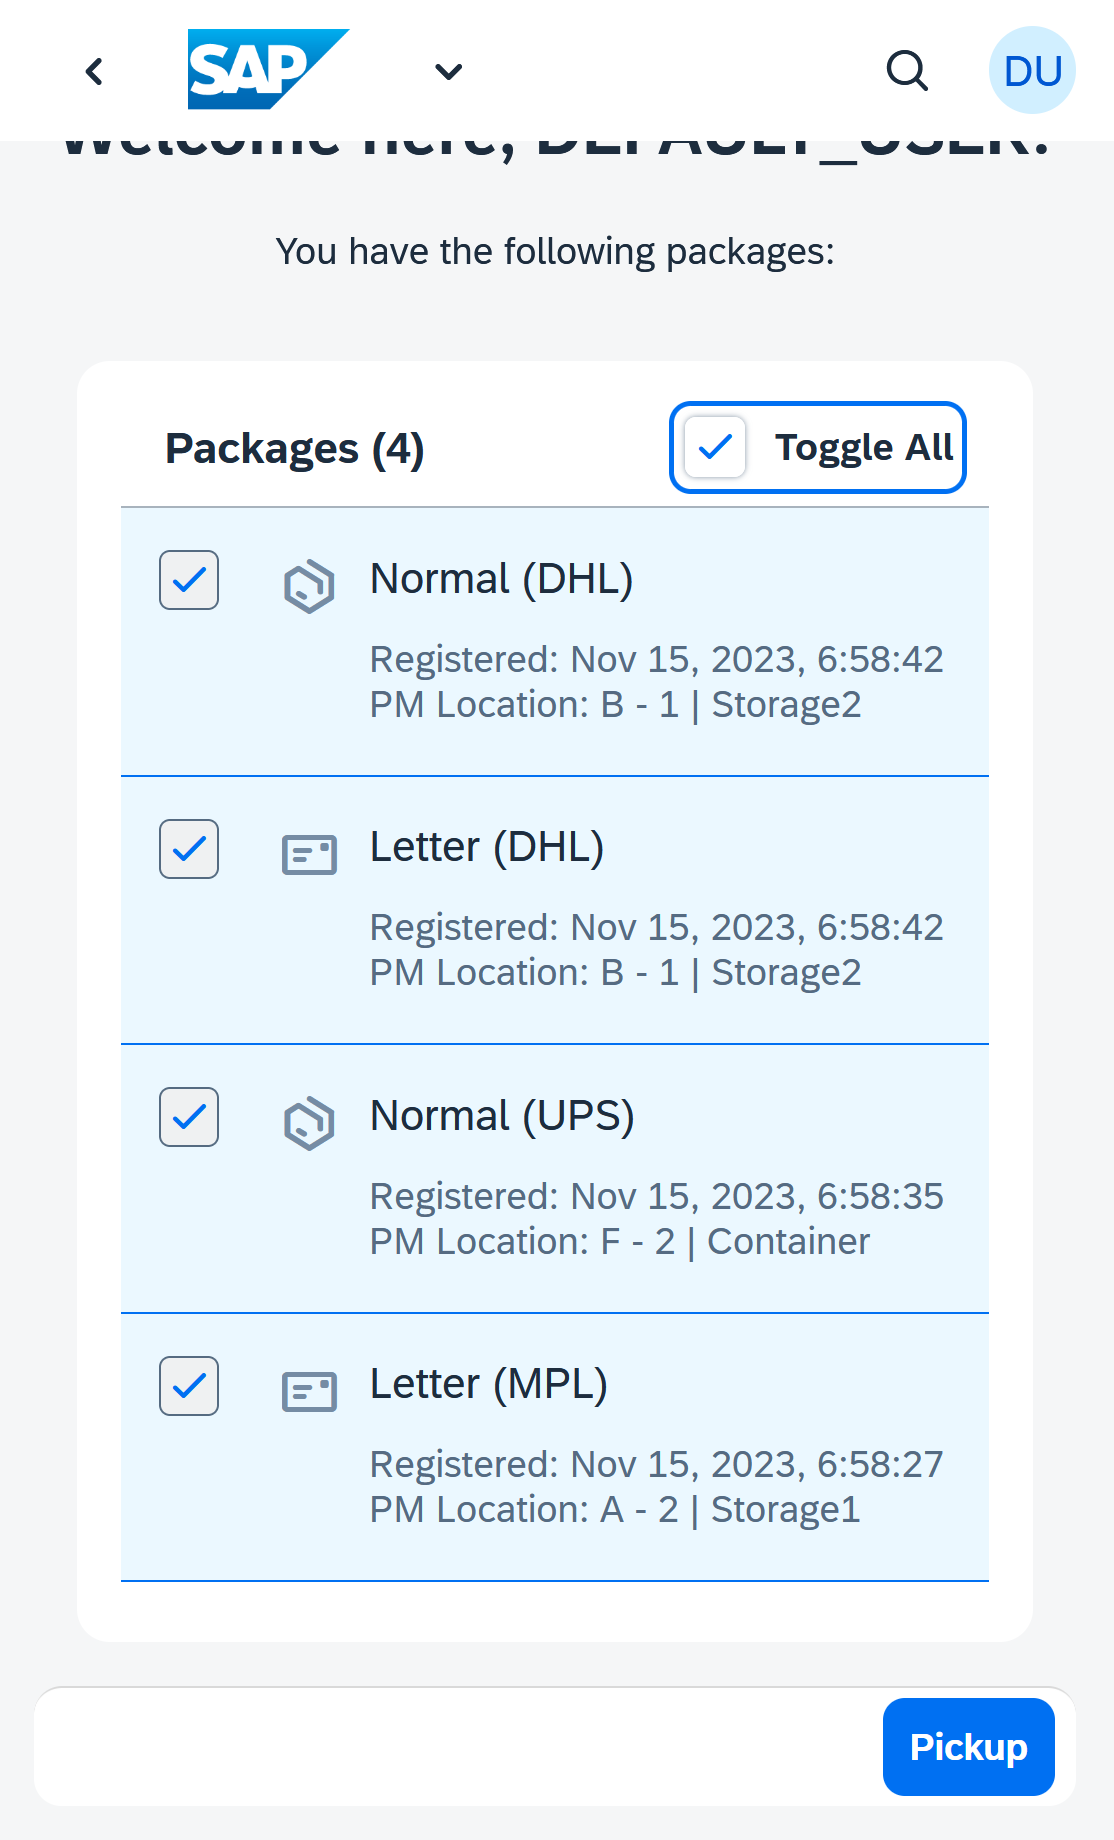
\includegraphics[height=260pt]{images/user_doc/pickup/HomeScreenToggleAll.png}}
% 	\hspace{5pt}
% 	\subcaptionbox{Home Screen Deselect All}{
% 		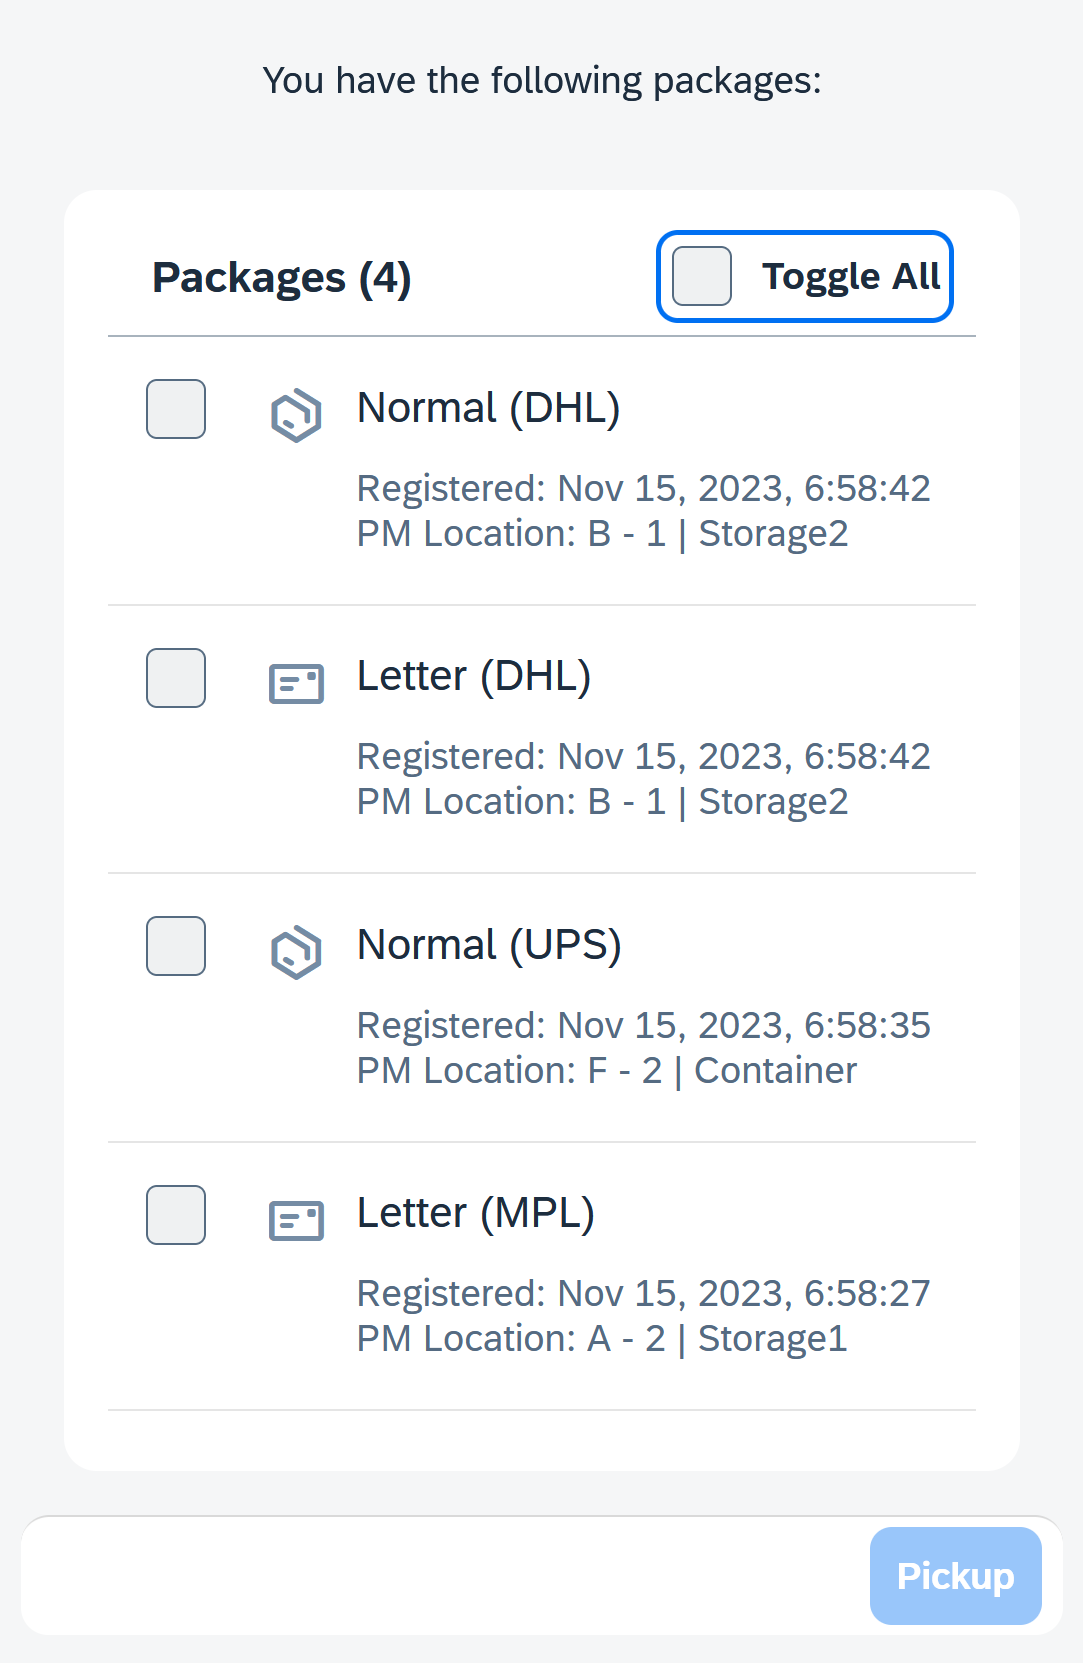
\includegraphics[height=260pt]{images/user_doc/pickup/HomeScreenDeToggleAll.png}}
% 	\caption{Pickup Home Screen - Selection Guide}
% 	\label{fig:PickupHomeScreen-2}
% \end{figure}

\subsubsection{Home Screen - Pickup}
The "Pickup" button at right bottom corner will only be enabled if at least one package is selected. In case it is enabled, one can pick up the selected packages by left clicking the "Pickup" button, which will trigger a confirmation dialog. If one choose "Cancel", the dialog closes and no modification is made. If one choose "OK", then all packages selected will be marked as pickup, removed from the list and the user will be navigated to the "Done Screen". At this point, the process of the picked up package will be closed, the package data will never be deleted and \textbf{End User} can always go to \textbf{My Packages} application to check the package history.

\begin{figure}[H]
	\centering
	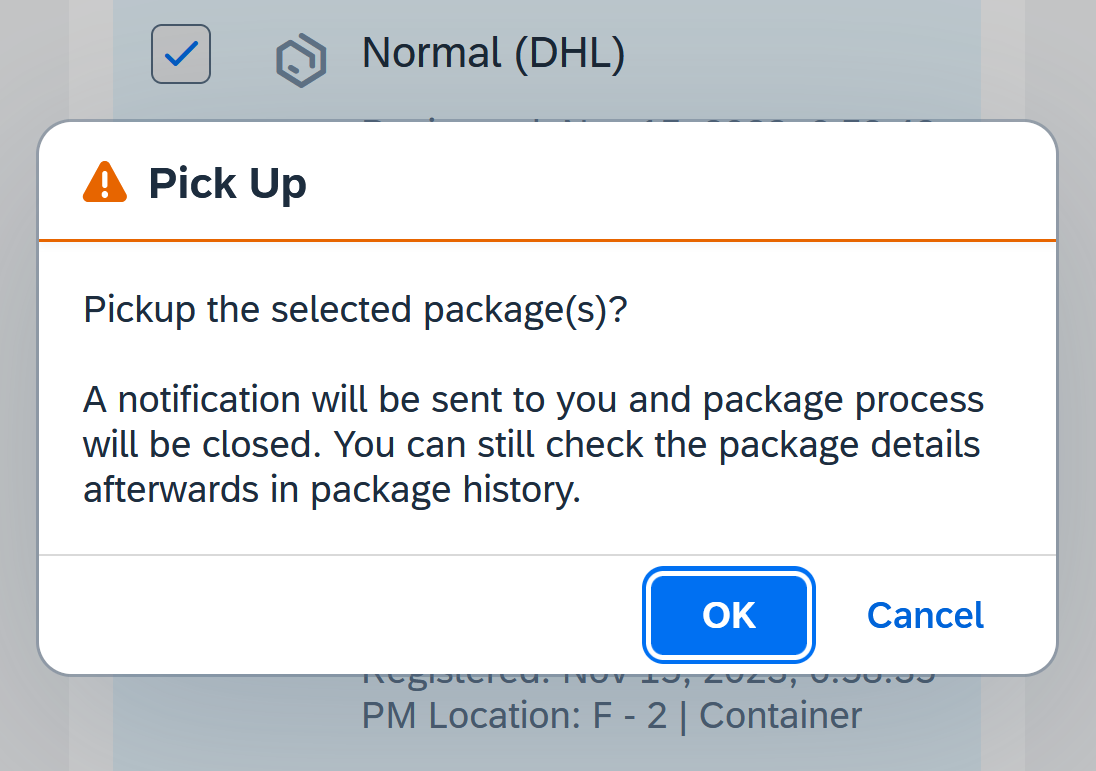
\includegraphics[height=200pt]{images/user_doc/pickup/PickupDialog.png}
	\caption{Pickup Home Screen - Pickup Dialog}
	\label{fig:PickupDialog}
\end{figure}

\subsubsection{Done Screen}

At the "Done Screen", if the \textbf{End User} still have packages to pickup, it will display the list of packages showing their \textbf{type with icon}, \textbf{delivery company} and \textbf{location info}. Otherwise, it displays no more packages. 
User can always navigate back to "Home Screen" by left clicking the "Close" button at the right bottom corner of the page.
From there, a new pickup iteration starts.

\begin{figure}[H]
	\centering
	\subcaptionbox{Done Screen with Packages}{
		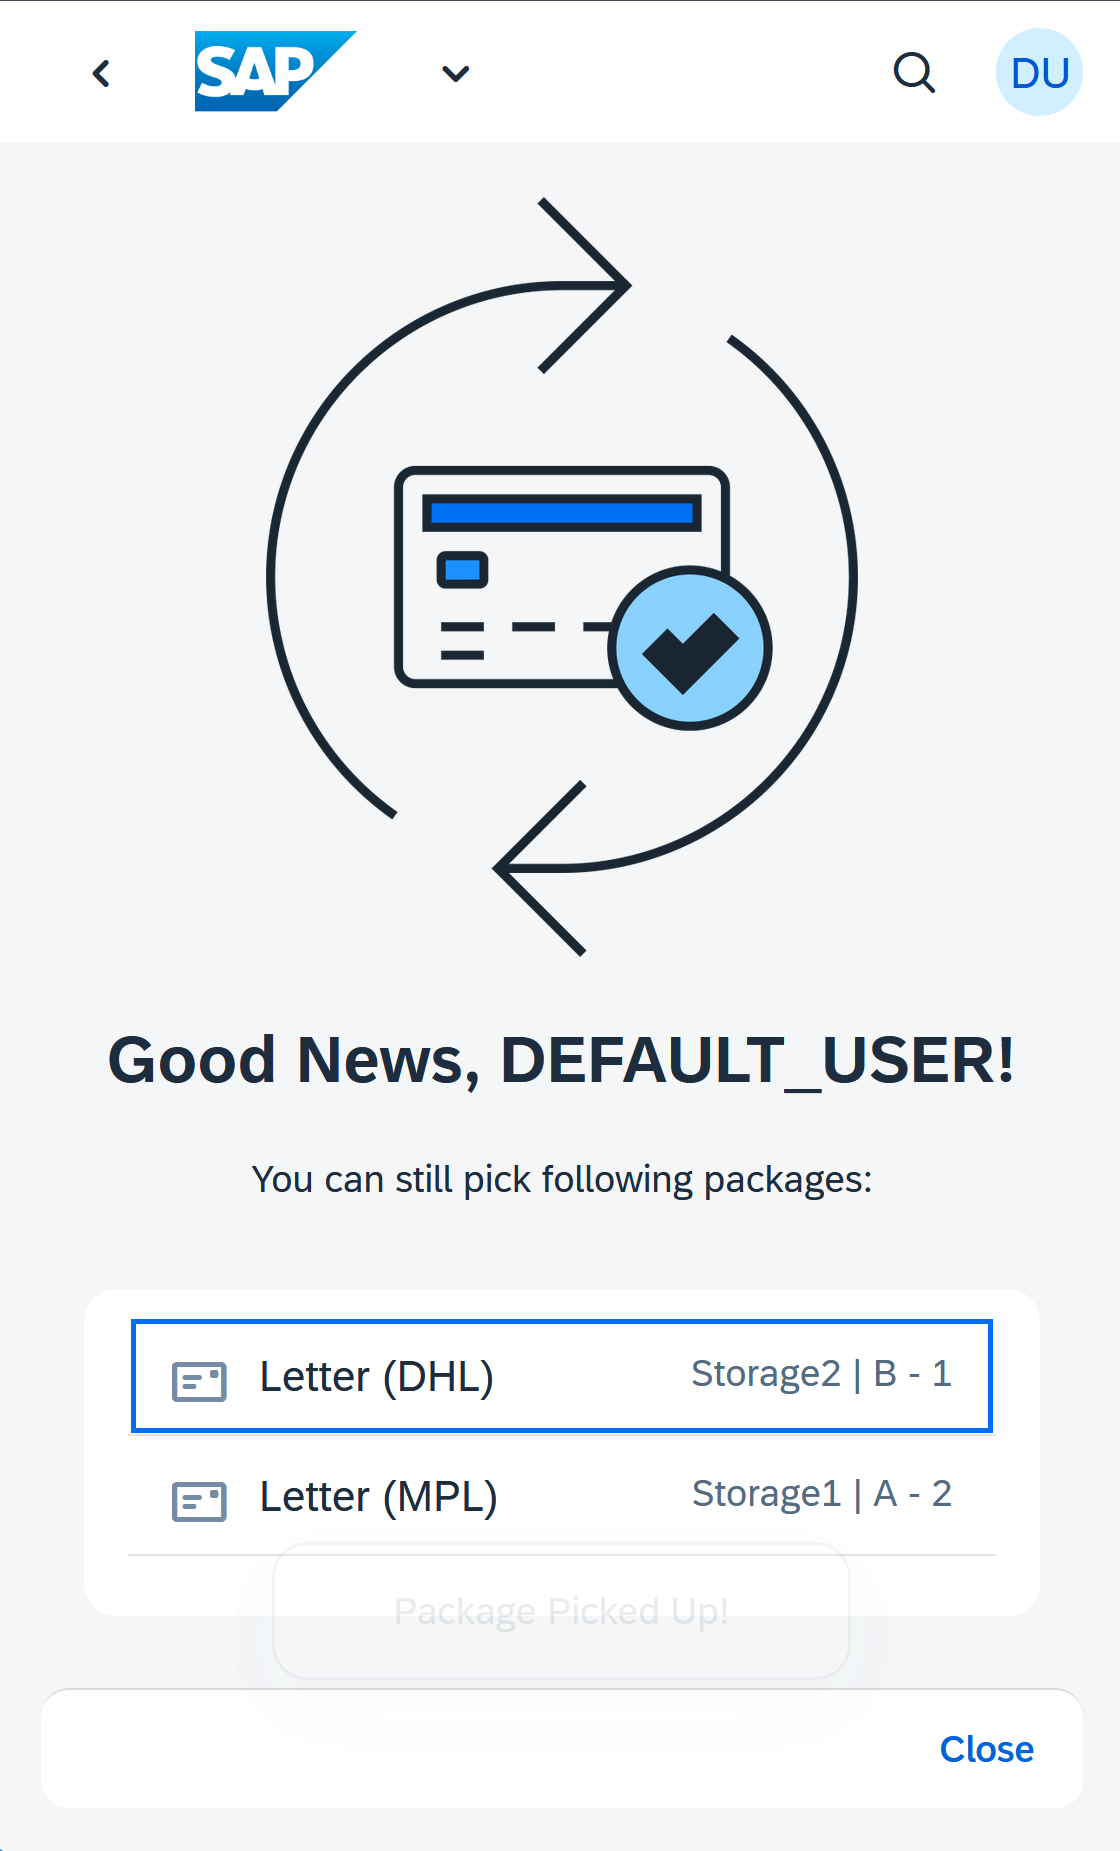
\includegraphics[width=0.45\linewidth]{images/user_doc/pickup/DoneScreenRemainPackages.png}}
	\hspace{5pt}
	\subcaptionbox{Done Screen without Packages}{
		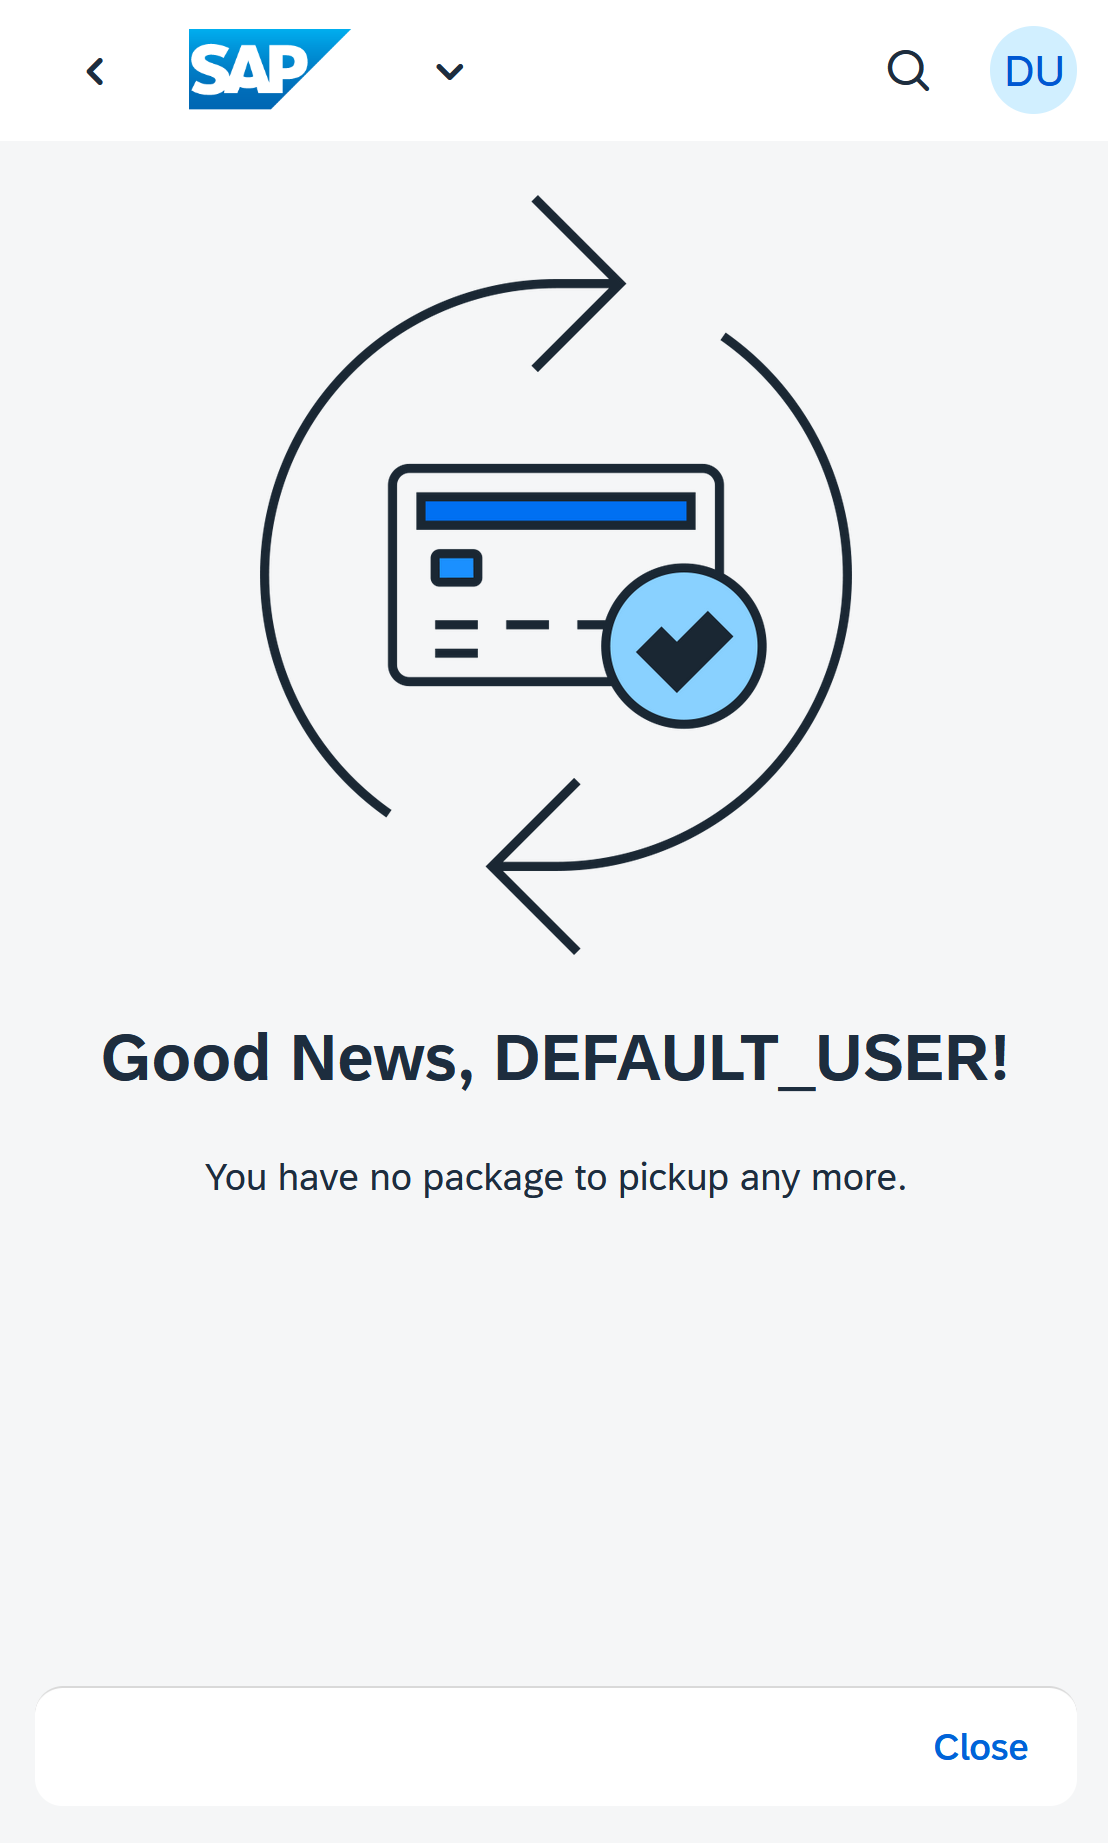
\includegraphics[width=0.45\linewidth]{images/user_doc/pickup/DoneScreenNoPackage.png}}
	\caption{Pickup Done Screen - Package Existence Guide}
	\label{fig:PickupHomeScreen-1}
\end{figure}

\pagebreak

\section{Receptionist}

As a logged in \textbf{Receptionist}, one is granted to access the two applications under the \textbf{Parcel Handling} section, namely \textbf{Register Packages} and \textbf{Manage Packages}. One can quick jump to the section by left clicking the "Parcel Handling" tab. One can enter the application by left click the tiles.

\begin{figure}[H]
	\centering
	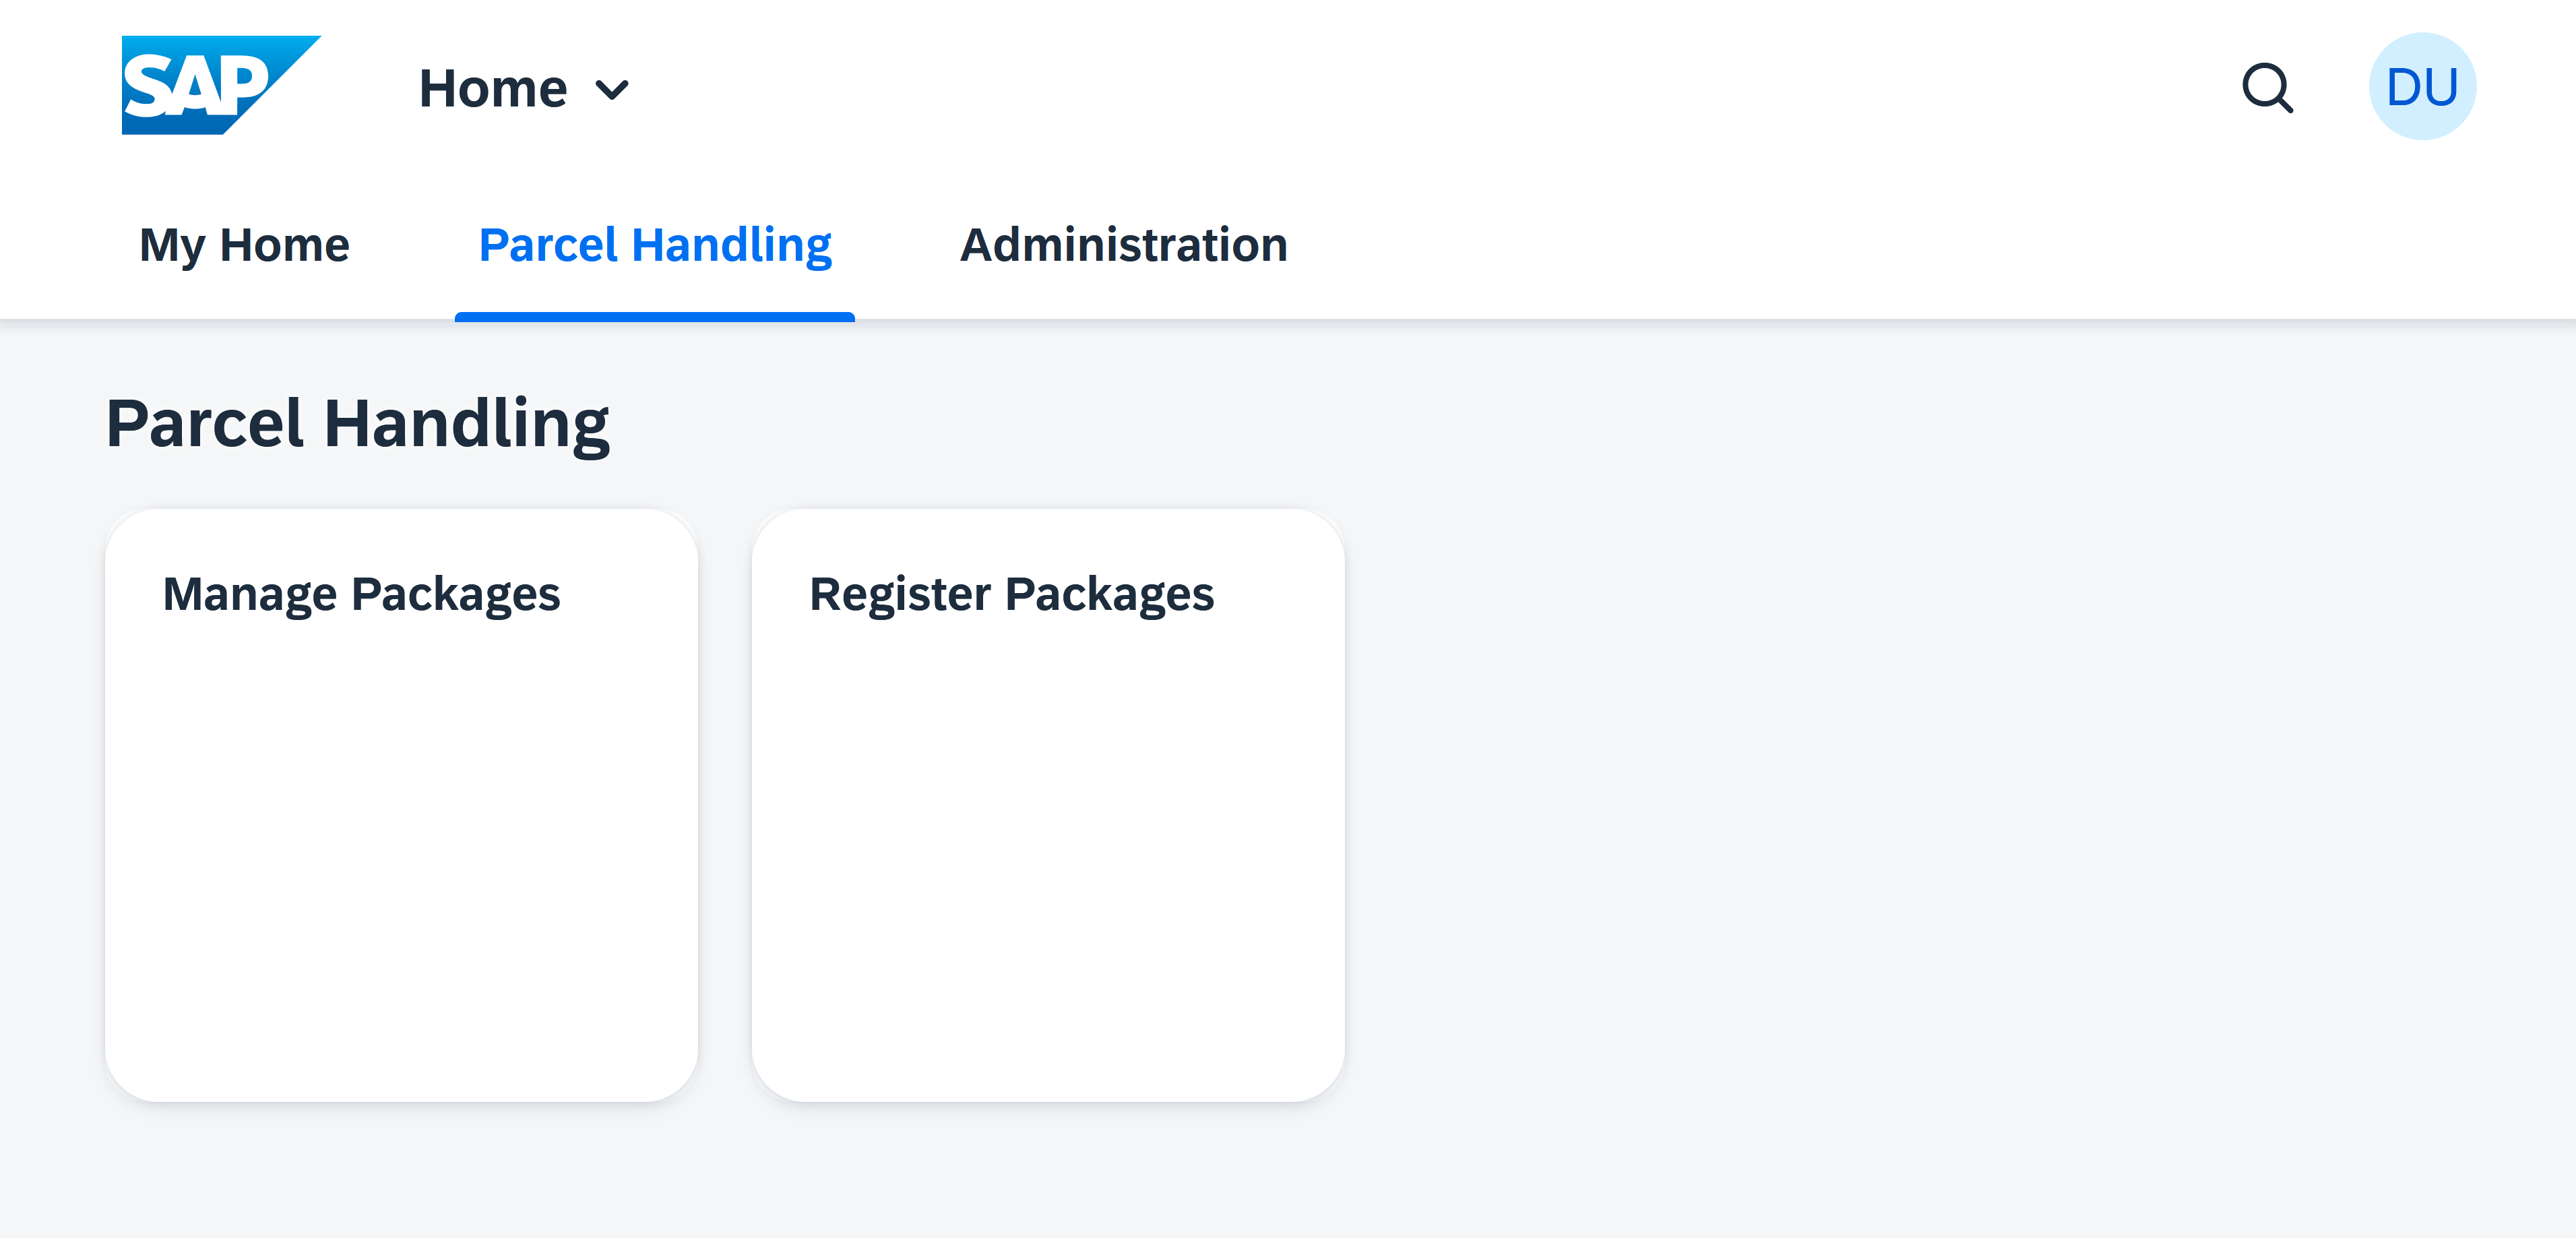
\includegraphics[width=1\linewidth]{images/user_doc/overviews/ParcelHandlingTab.png}
	\caption{Parcel Handling Applications}
	\label{fig:PHApplications}
\end{figure}


\subsection{Register Packages}

\subsection{Manage Packages}                     

\begin{figure}[H]
	\centering
	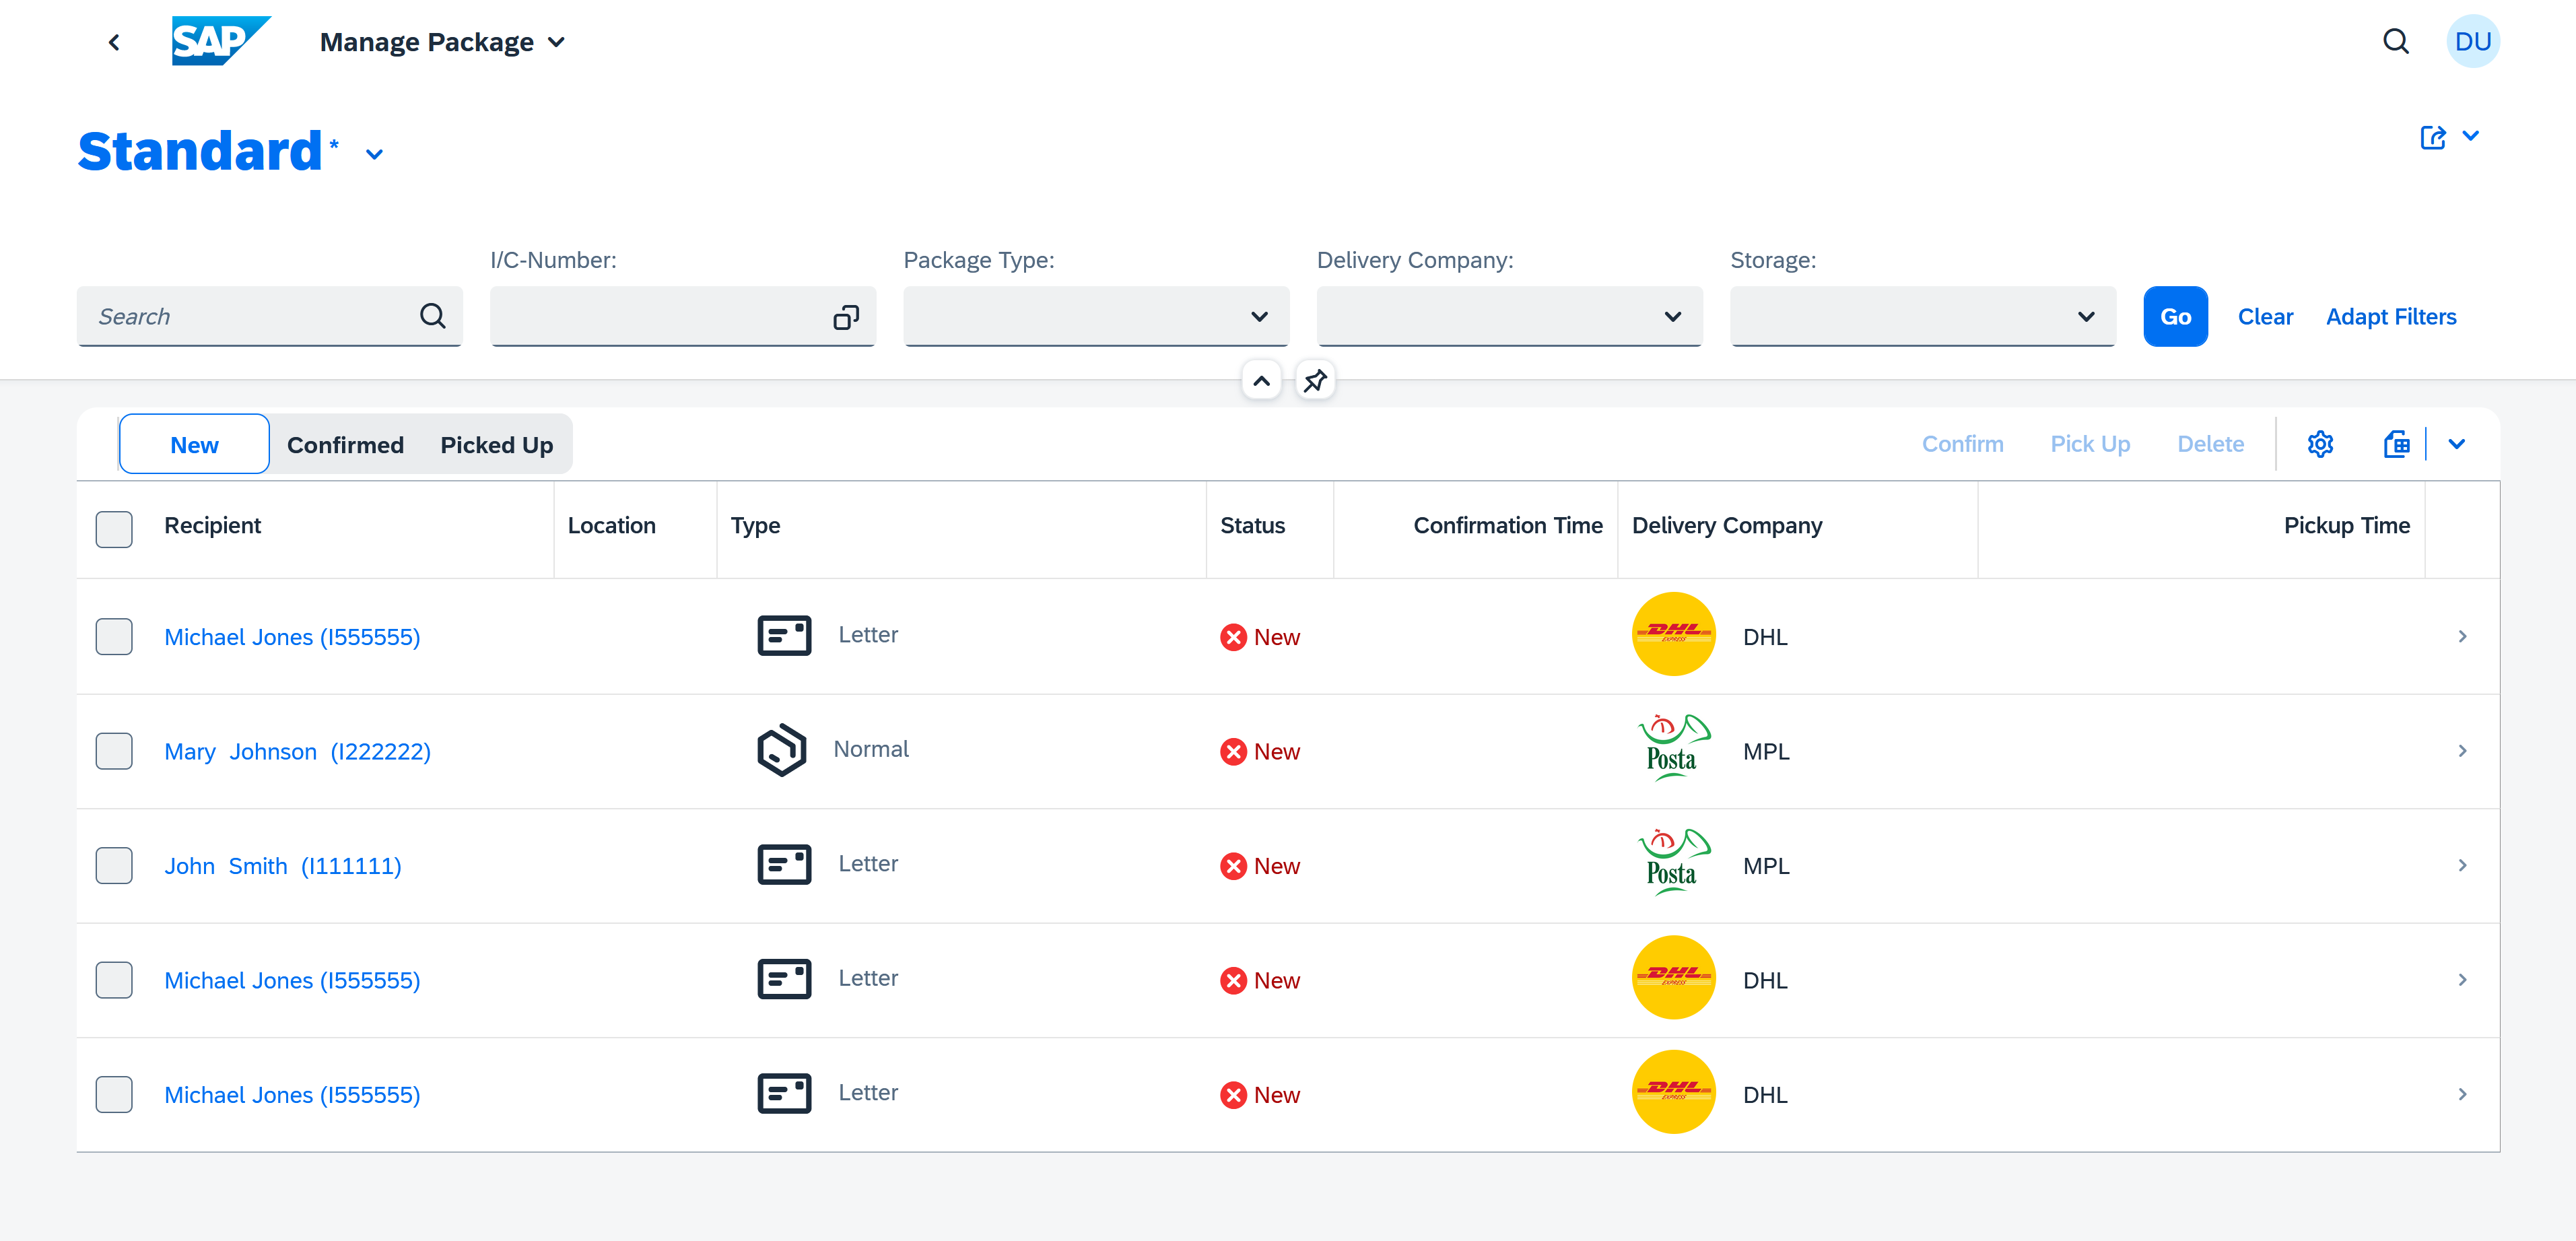
\includegraphics[height=200pt]{images/user_doc/managePack/ReportScreen/browse/Overview.png}
	\caption{Manage Packages Report Screen - Overview}
	\label{fig:PickupDialog}
\end{figure}

The \textbf{Manage Packages} application is designed for \textbf{Receptionist} to edit, confirm, pickup, check the existing packages in the system. The summarized main actions a \textbf{Receptionist} can take are listed here:

\begin{compactenum}
	\item Browse the existing packages.
        \begin{compactenum}
            \item Filtering possibility.
            \item Quick variant switch based on package status.
            \item Report List of packages info with selection capability.
            \item Detail page for single packages.
        \end{compactenum}
    \item Confirm package(s) which status is new.
    \item Pickup a package (single at a time) which status is confirmed. (As a backup manuvor in case the employee cannot access to mobile devices.
    \item Delete package(s) which status is new or confirmed.
    \item Edit package(s)' recipient, type, delivery company, and comment.
\end{compactenum}
\bigskip

Further explanation and restrictions of these operations are detailed in the coming sections.


\subsubsection{Browse}
As an \textbf{Receptionist}, after clicking at the application tile, is redirected to the "Report Screen", which is the main screen of this application. 
The upper part displays the search bar and the possible filters. 
In case the need of free text search of any possible content of the column, one can use the \textbf{"Search Bar"}. The search supports in-completed keywords and is case insensitive. One can also use the predefined filters, where value helps and entry helps are provided.
The default predefined filters are: \textbf{I/C-Number} (free text SAP ID input), \textbf{Type} (drop down of all available types), \textbf{Delivery Company} (drop down of all available companies) and \textbf{Storage} (drop down of all available storage). 
For drop down filters, one can click at the small drop down arrow and select zero to many options. When adjusting the filtering values, the list view is temporarily locked. After adjusting the filtering values, one can run and review the filter result by clicking the "Go" Button.

\begin{figure}[H]
	\centering
	
\includegraphics[width=1\linewidth]{images/user_doc/managePack/ReportScreen/browse/FilterBar.png}
	\caption{Manage Packages Report Screen - Filter Bar}
	\label{fig:MPFIlterBar}
\end{figure}

\begin{figure}[H]
	\centering
	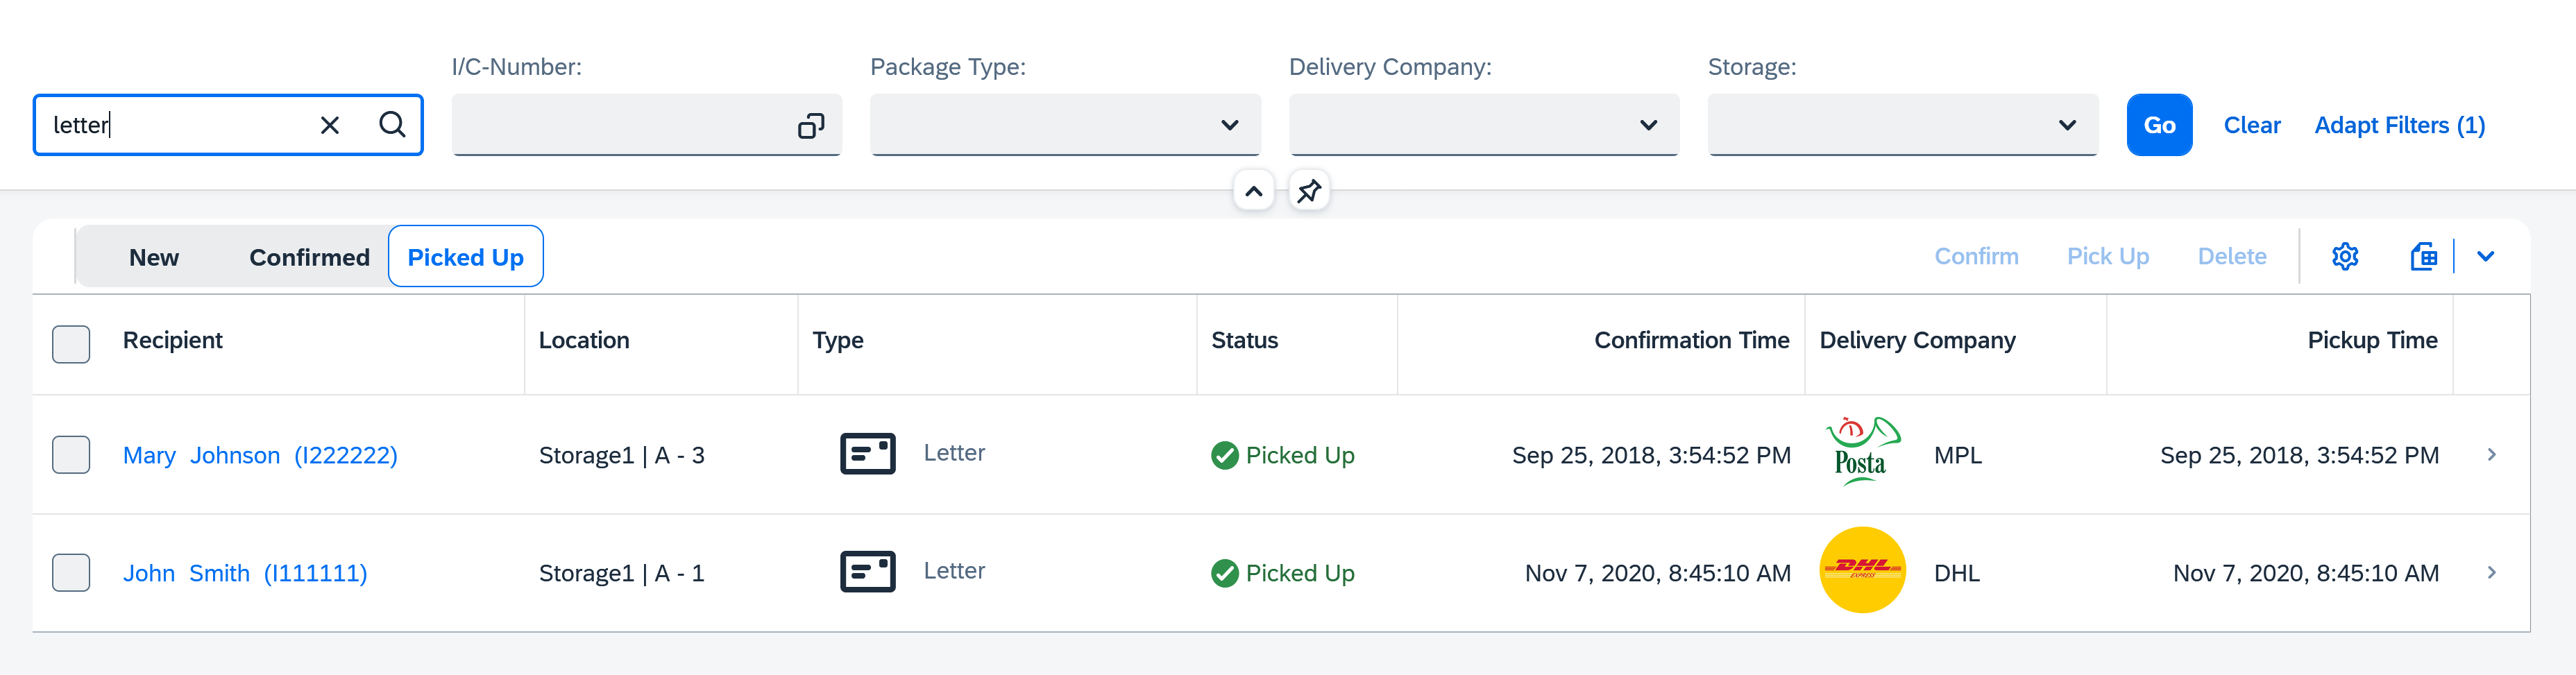
\includegraphics[width=1\linewidth]{images/user_doc/managePack/ReportScreen/browse/defaultSearchBarUsage.png}
	\caption{Manage Packages Report Screen - Filter Bar - Search Bar Usage Guide}
	\label{fig:MPSearchBar}
\end{figure}

\begin{figure}[H]
	\centering
	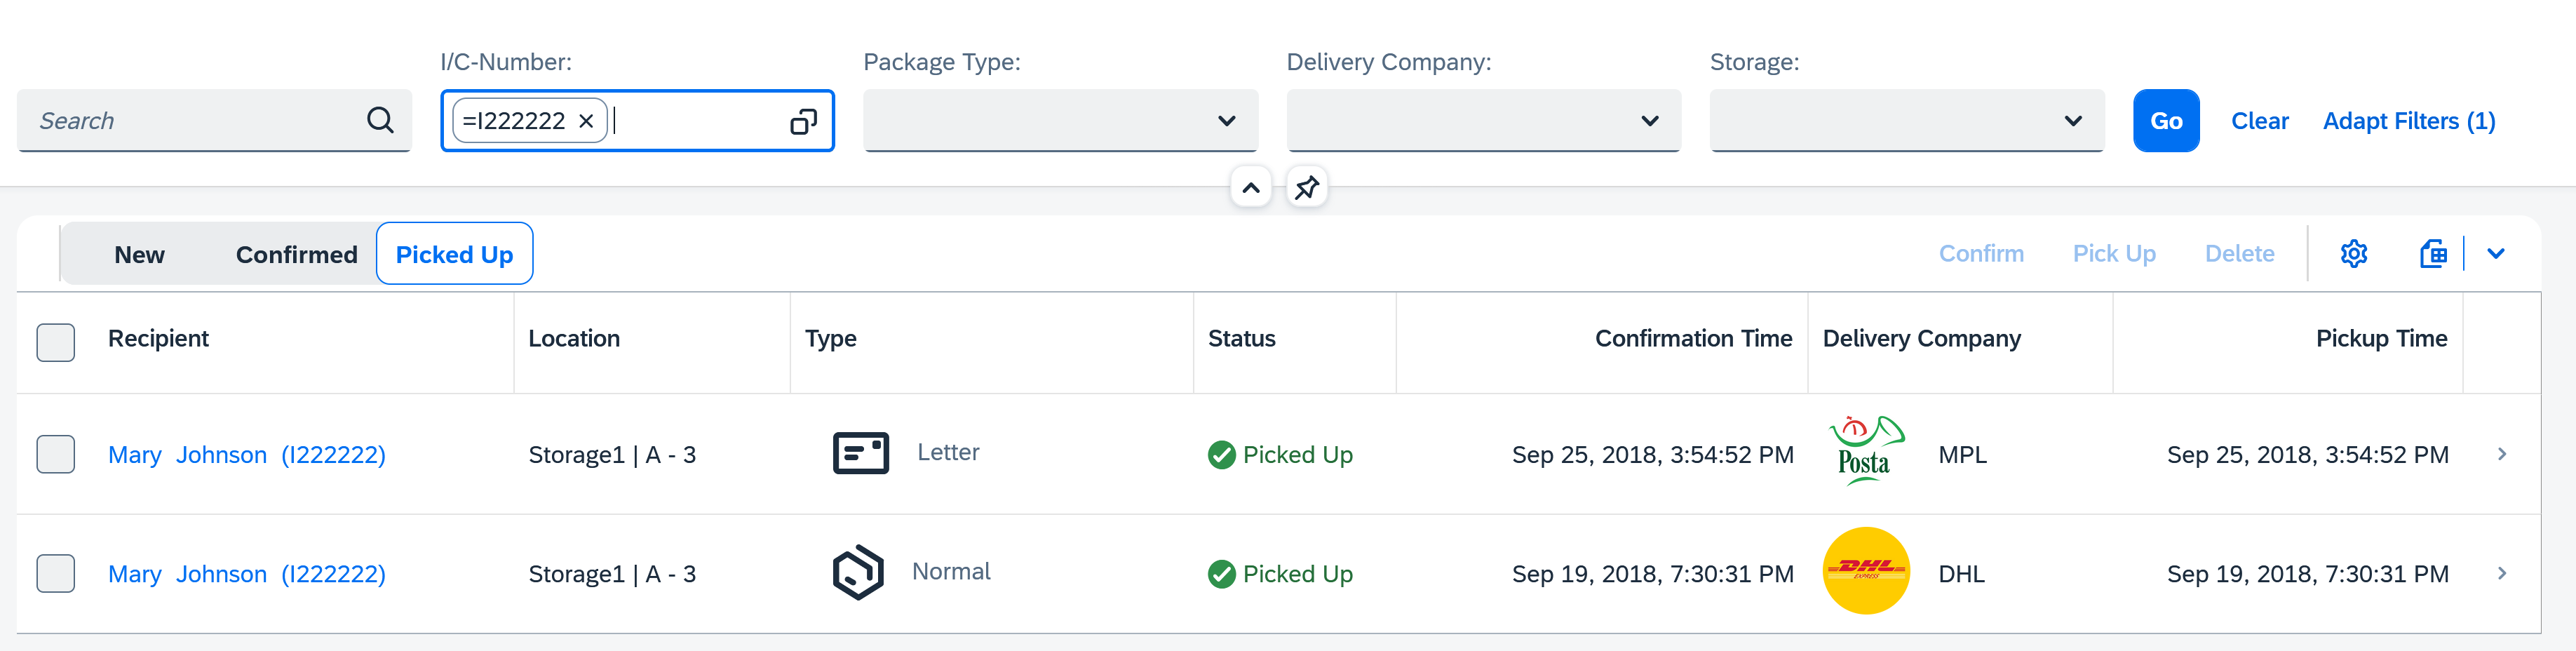
\includegraphics[width=1\linewidth]{images/user_doc/managePack/ReportScreen/browse/defaultFreeTextIdUsage.png}
	\caption{Manage Packages Report Screen - Filter Bar - ID Filter Usage Guide}
	\label{fig:MPIDFIlter}
\end{figure}

\begin{figure}[H]
	\centering
	\subcaptionbox{Type Filter}{
		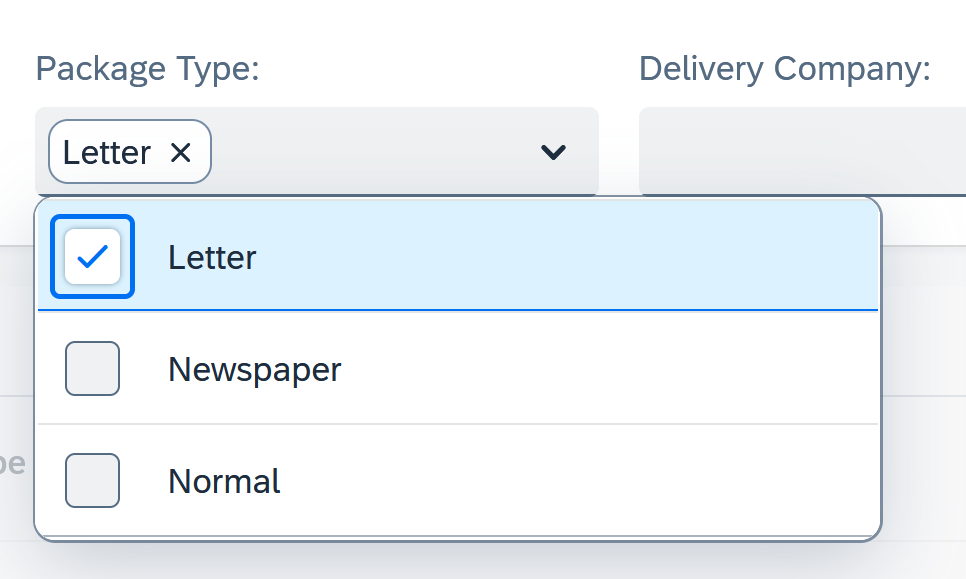
\includegraphics[width=0.45\linewidth]{images/user_doc/managePack/ReportScreen/browse/defaultType.png}}
	\hspace{5pt}
	\subcaptionbox{Company Filter}{
		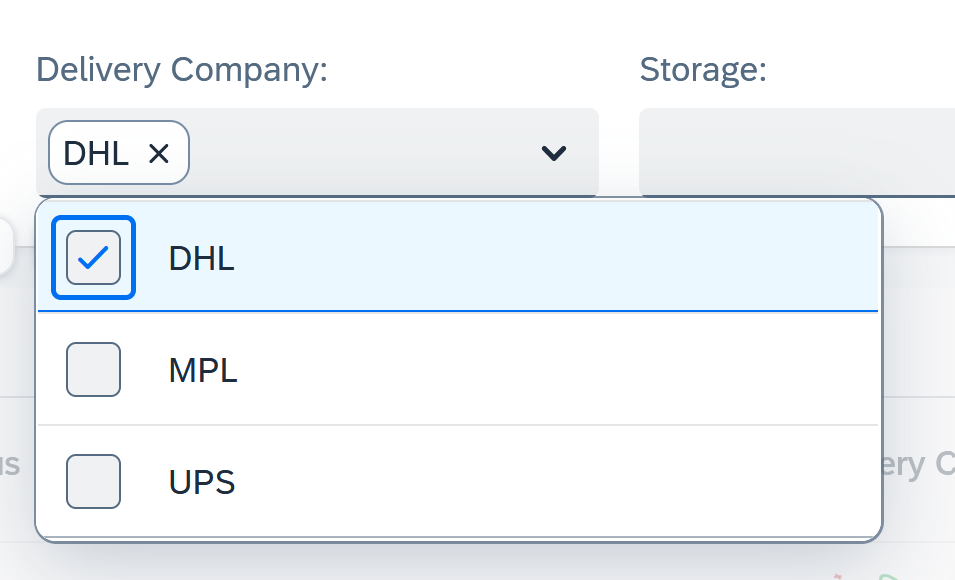
\includegraphics[width=0.45\linewidth]{images/user_doc/managePack/ReportScreen/browse/defaultCompany.png}}

    \subcaptionbox{Storage Filter}{
		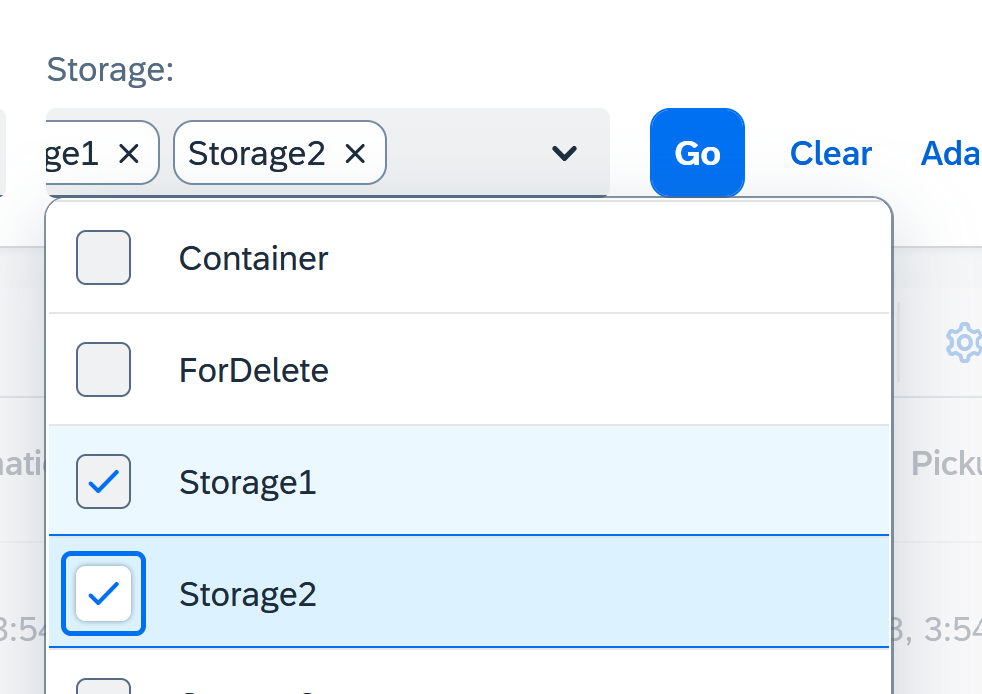
\includegraphics[width=0.45\linewidth]{images/user_doc/managePack/ReportScreen/browse/defaultStorage.png}}
	\caption{Manage Packages Report Screen - Filter Bar - Default Drop Down Filters Show Case}
	\label{fig:MPDefaultDropDown}
\end{figure}

In the middle there is a variant bread cum on the left and three action buttons on the right. The variant breadcrumb shows the three possible status of the packages. When clicking on one of the variants, the list of packages with corresponding status are displayed. The three action buttons are by default inactivated. They will be activated when certain conditions are full filled (i.e. the action can be performed).

\begin{figure}[H]
	\centering
	\subcaptionbox{Variants Bread}{
		
\includegraphics[width=0.45\linewidth]{images/user_doc/managePack/ReportScreen/browse/VariantsBread.png}}
	\hspace{5pt}
	\subcaptionbox{Action Buttons}{
		
\includegraphics[width=0.45\linewidth]{images/user_doc/managePack/ReportScreen/browse/buttonInactive.png}}
  \caption{Manage Packages Report Screen - Middle Control}
	\label{fig:MPMiddle}
\end{figure}

\begin{figure}[H]
	\centering
	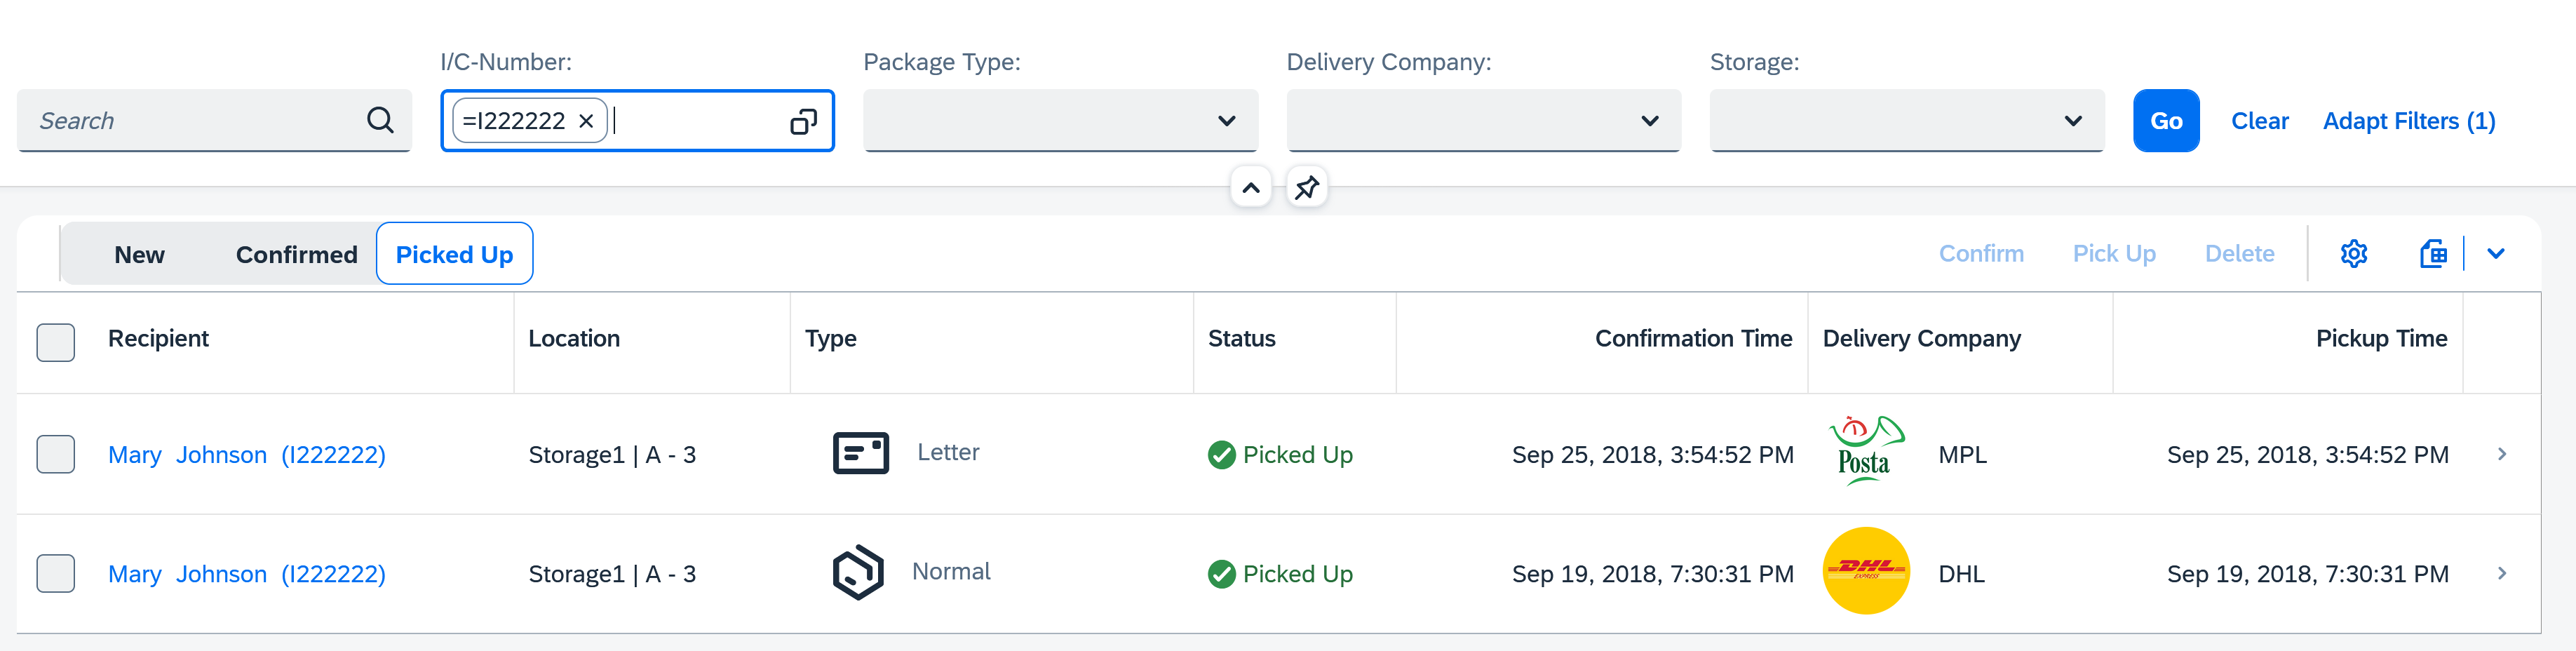
\includegraphics[width=1\linewidth]{images/user_doc/managePack/ReportScreen/browse/defaultFreeTextIdUsage.png}
	\caption{Manage Packages Report Screen - Middle Control - Breadcrumb Show Case}
	\label{fig:MPIDFIlter}
\end{figure}


\begin{figure}[H]
	\centering
	\subcaptionbox{New Variant}{
		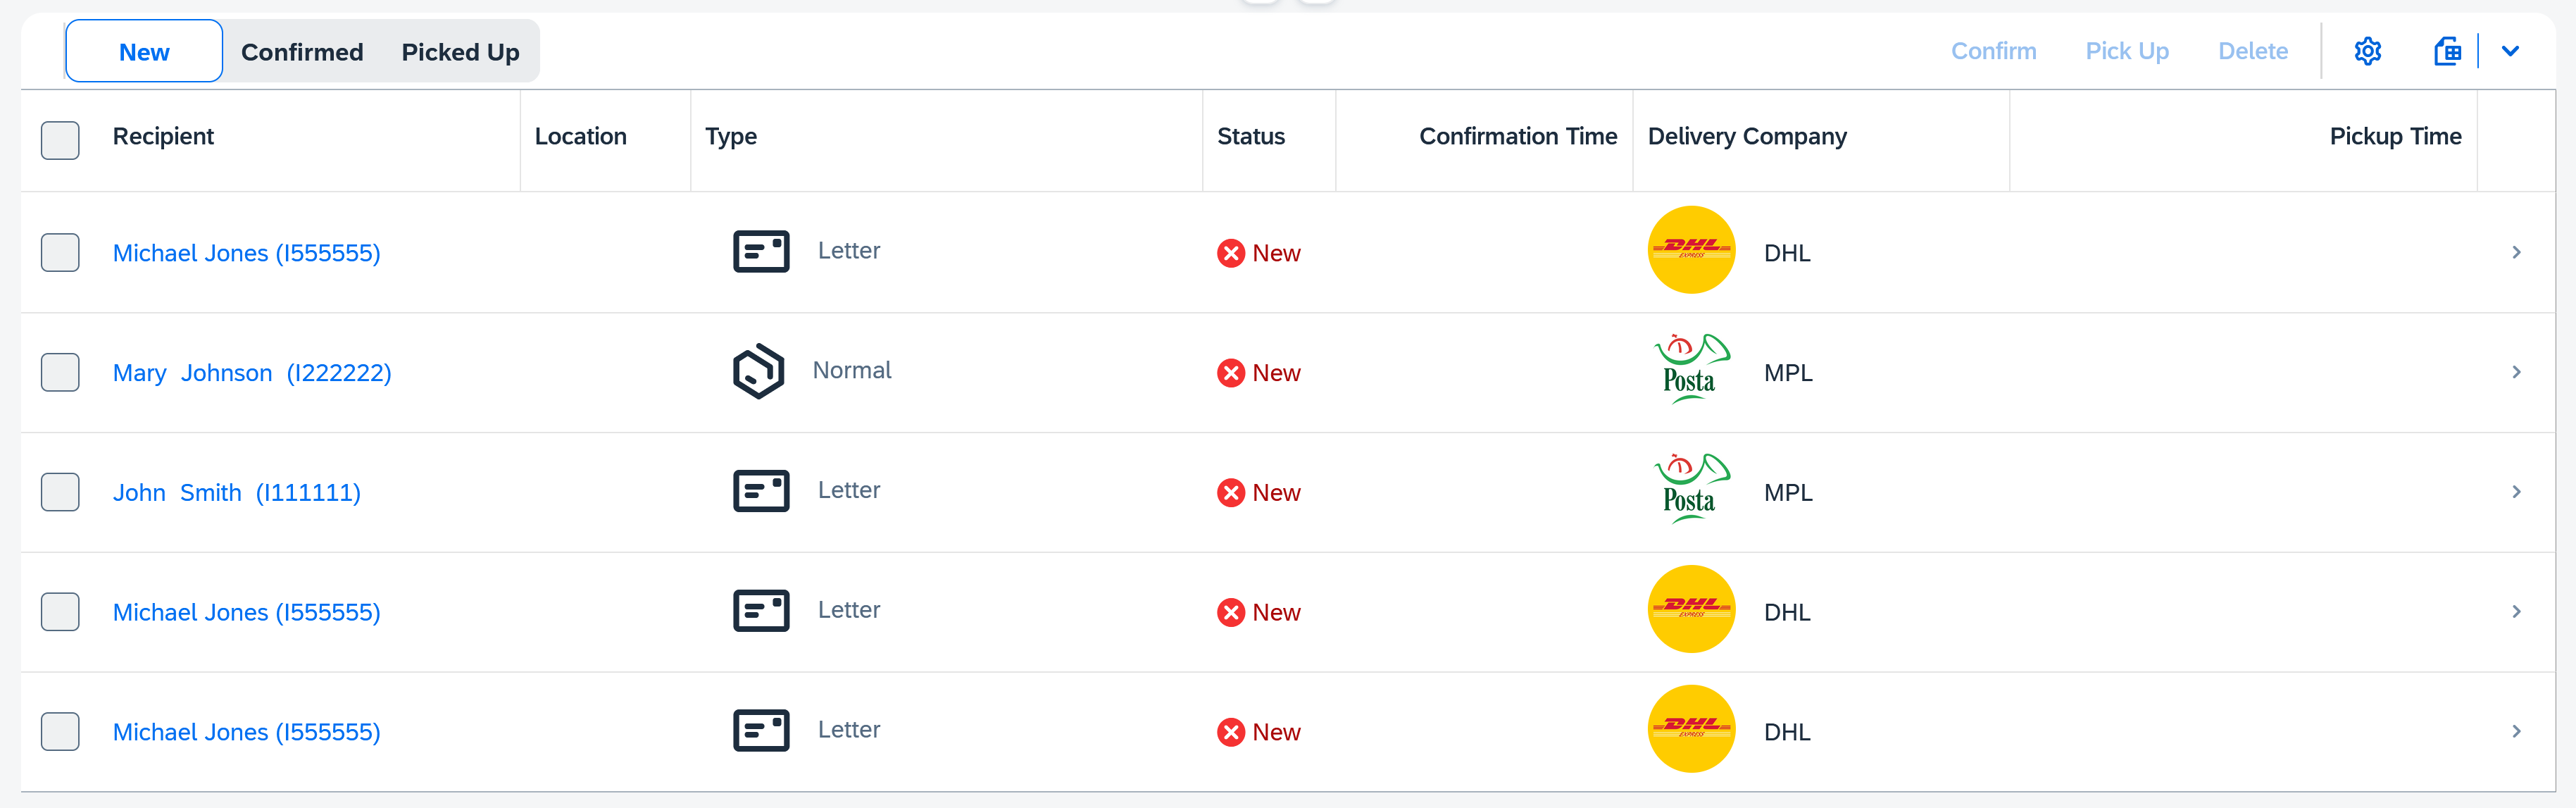
\includegraphics[width=0.45\linewidth]{images/user_doc/managePack/ReportScreen/browse/NewVariant.png}}
	\hspace{5pt}
	\subcaptionbox{Confirmed Variant}{
		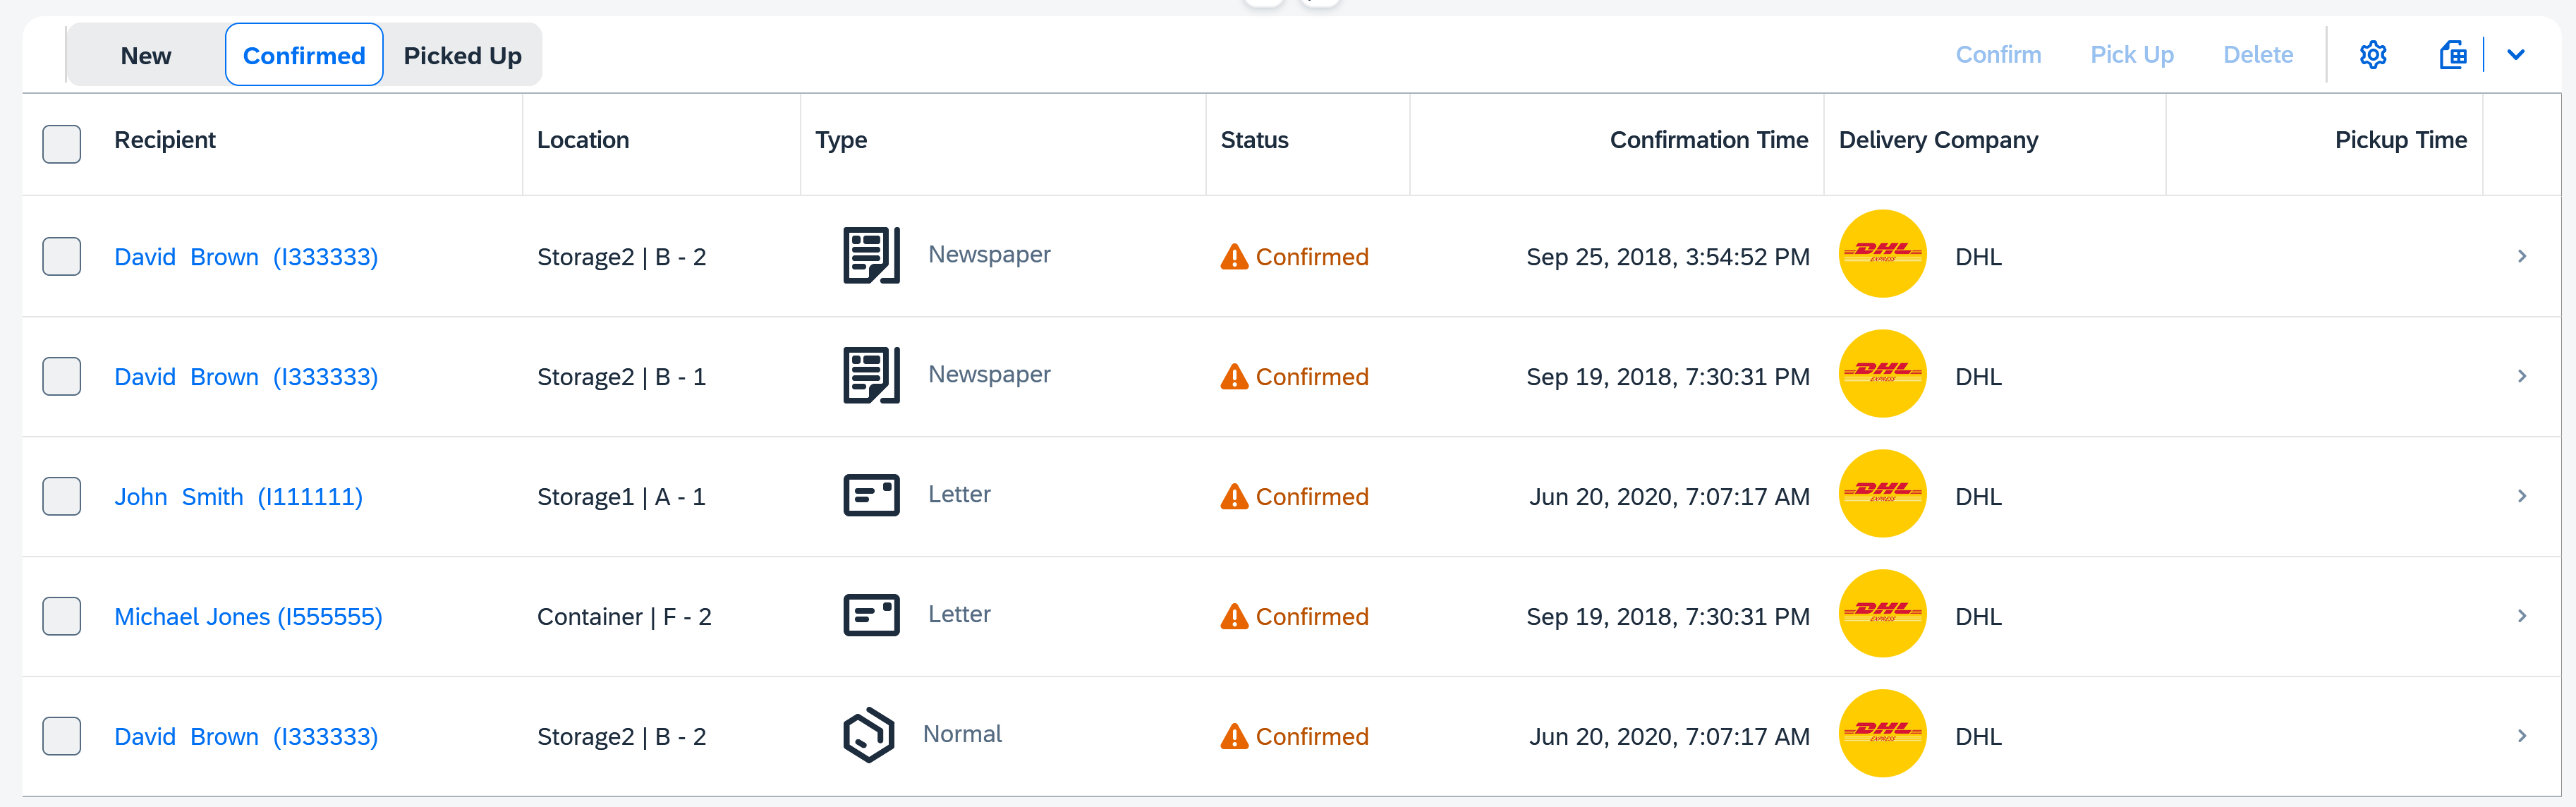
\includegraphics[width=0.45\linewidth]{images/user_doc/managePack/ReportScreen/browse/ConfirmedVariant.png}}

    \subcaptionbox{Picked Up Variant}{
		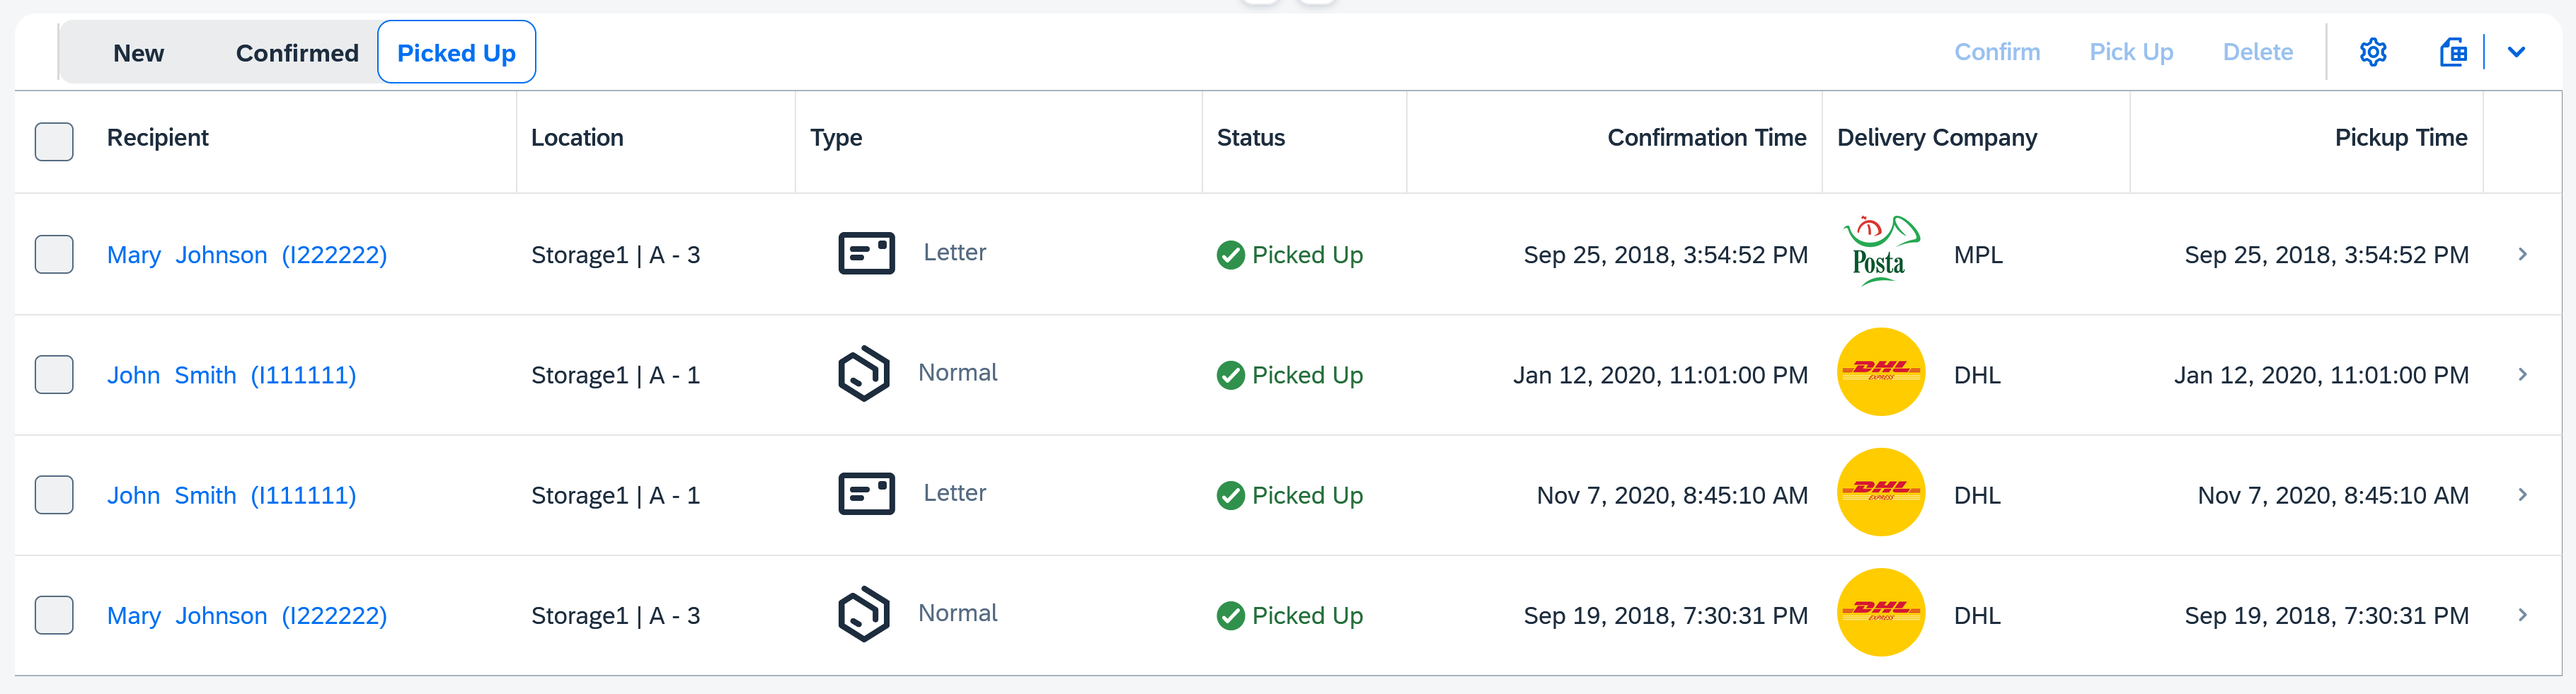
\includegraphics[width=0.45\linewidth]{images/user_doc/managePack/ReportScreen/browse/pickedupVariant.png}}
	\caption{Manage Packages Report Screen - Middle Control - Breadcrumb Show Case}
	\label{fig:MPBreadCrumb}
\end{figure}

The lower part displays the list of packages. The information provides for each packages are: \textbf{Recipient} (the recipient info, full name and SAP ID), \textbf{Location} (the storage and storage slot info of the package, if applicable), \textbf{Type} (the type of the package, existing types are newspaper, letter and normal), \textbf{Status} (the status of the package, existing status are new, confirmed and picked up), \textbf{Delivery Company} (the delivery company of the package), \textbf{Confirmation Time} (the confirmation time of the package, if applicable), \textbf{Pickup Time} (the picked up time of the package, if applicable).
In case selection of package is needed, one can select a package by ticking the selection box before the listed package item. One can also select and de-select all packages by toggling the selection box at the left corner of the list header.
In case contact info is needed for certain recipient, one can click at the \textbf{recipient}, a pop up contact card will display the email and phone number of the recipient.

\begin{figure}[H]
	\centering
	\subcaptionbox{Select All}{
		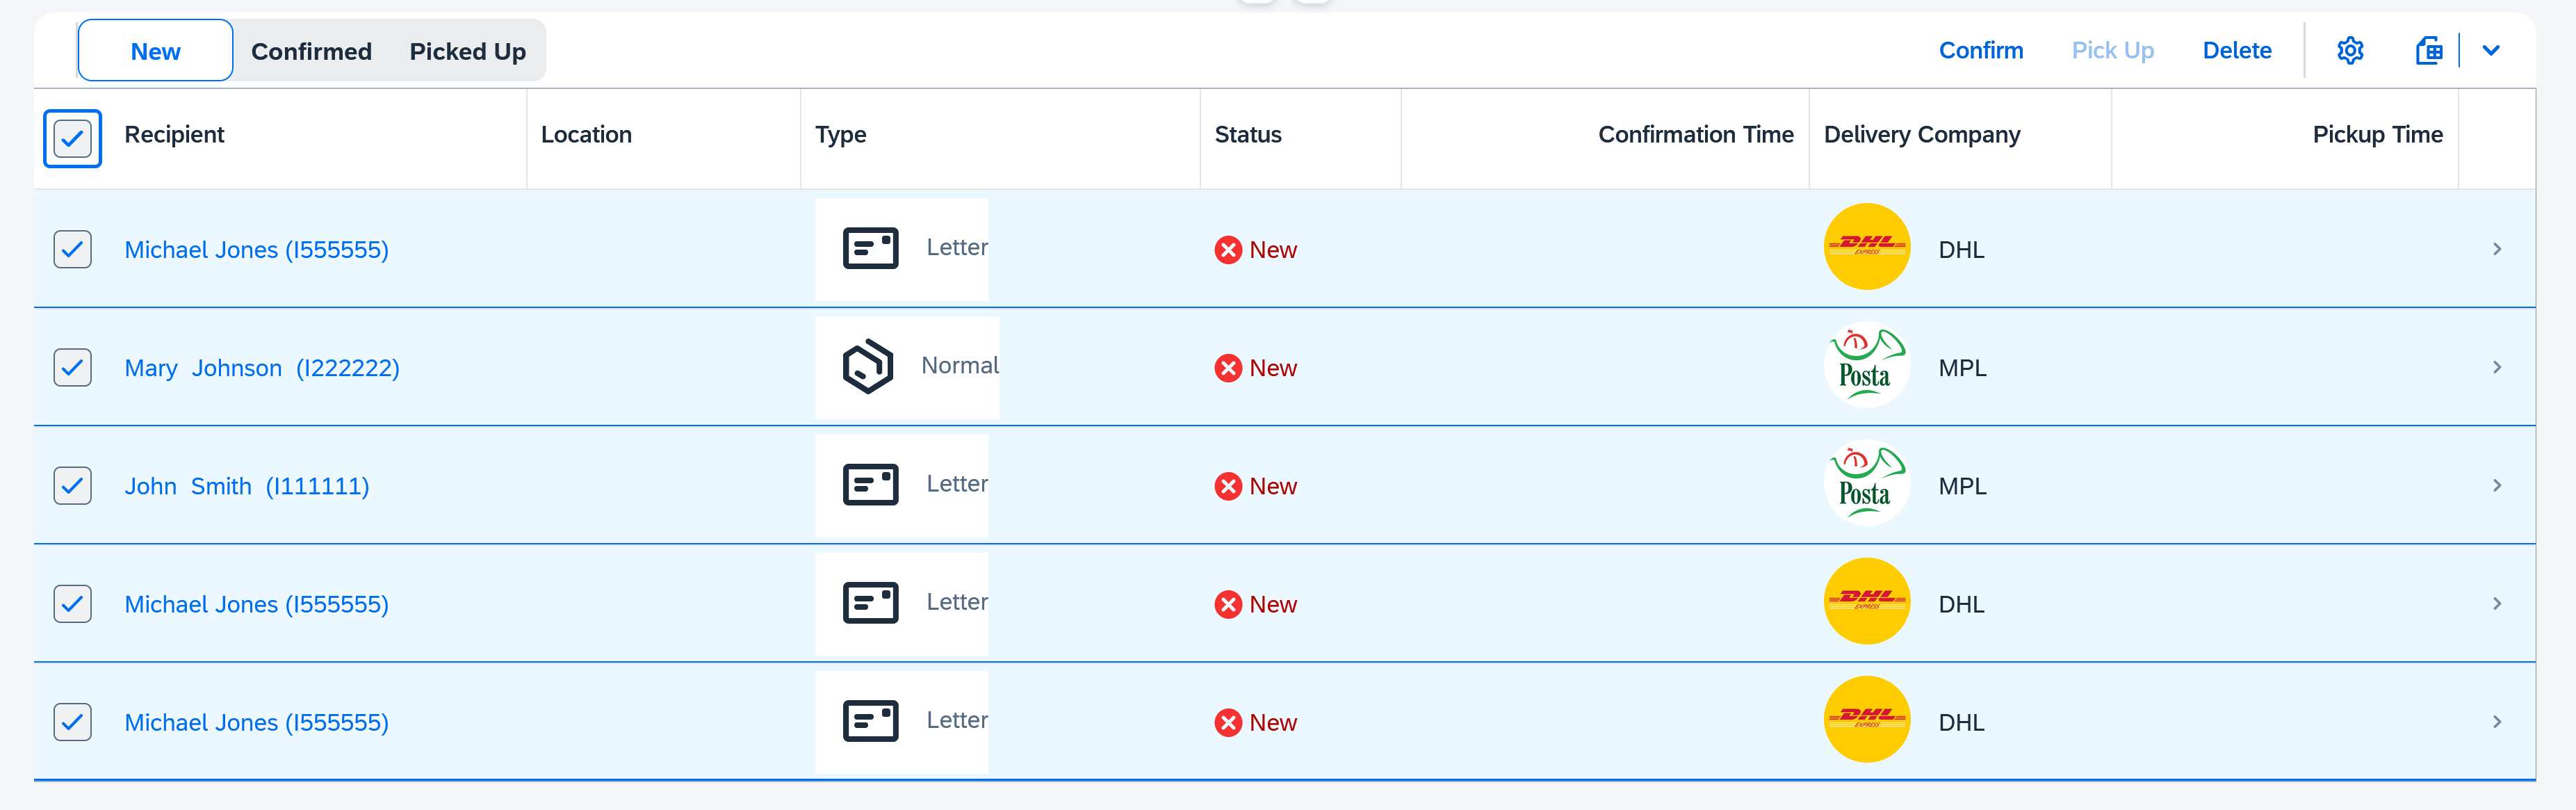
\includegraphics[width=0.45\linewidth]{images/user_doc/managePack/ReportScreen/browse/listSelectAll.png}}
	\hspace{5pt}
	\subcaptionbox{Deselect All}{
		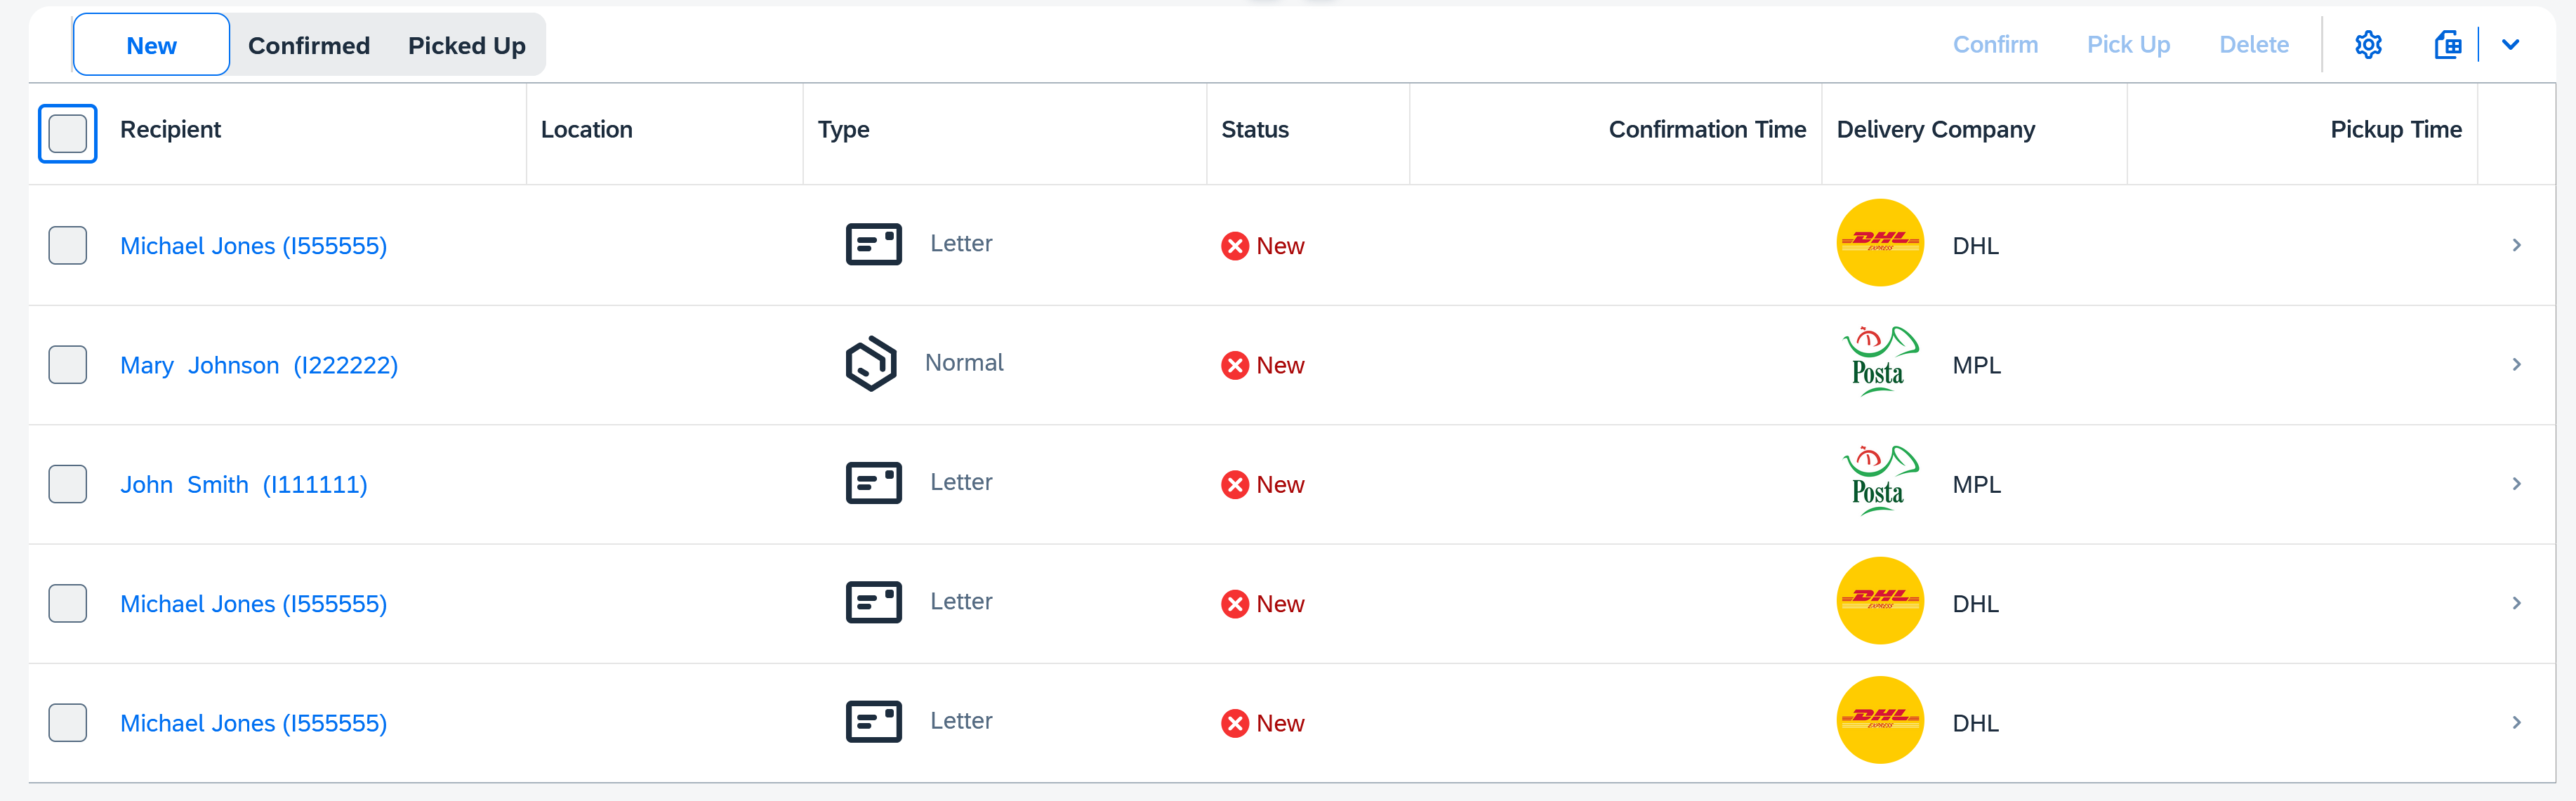
\includegraphics[width=0.45\linewidth]{images/user_doc/managePack/ReportScreen/browse/listDeSelectAll.png}}
    \caption{Manage Packages Report Screen - Report List - Selection Show Case}
	\label{fig:MPListSelection}
\end{figure}

\begin{figure}[H]
	\centering
	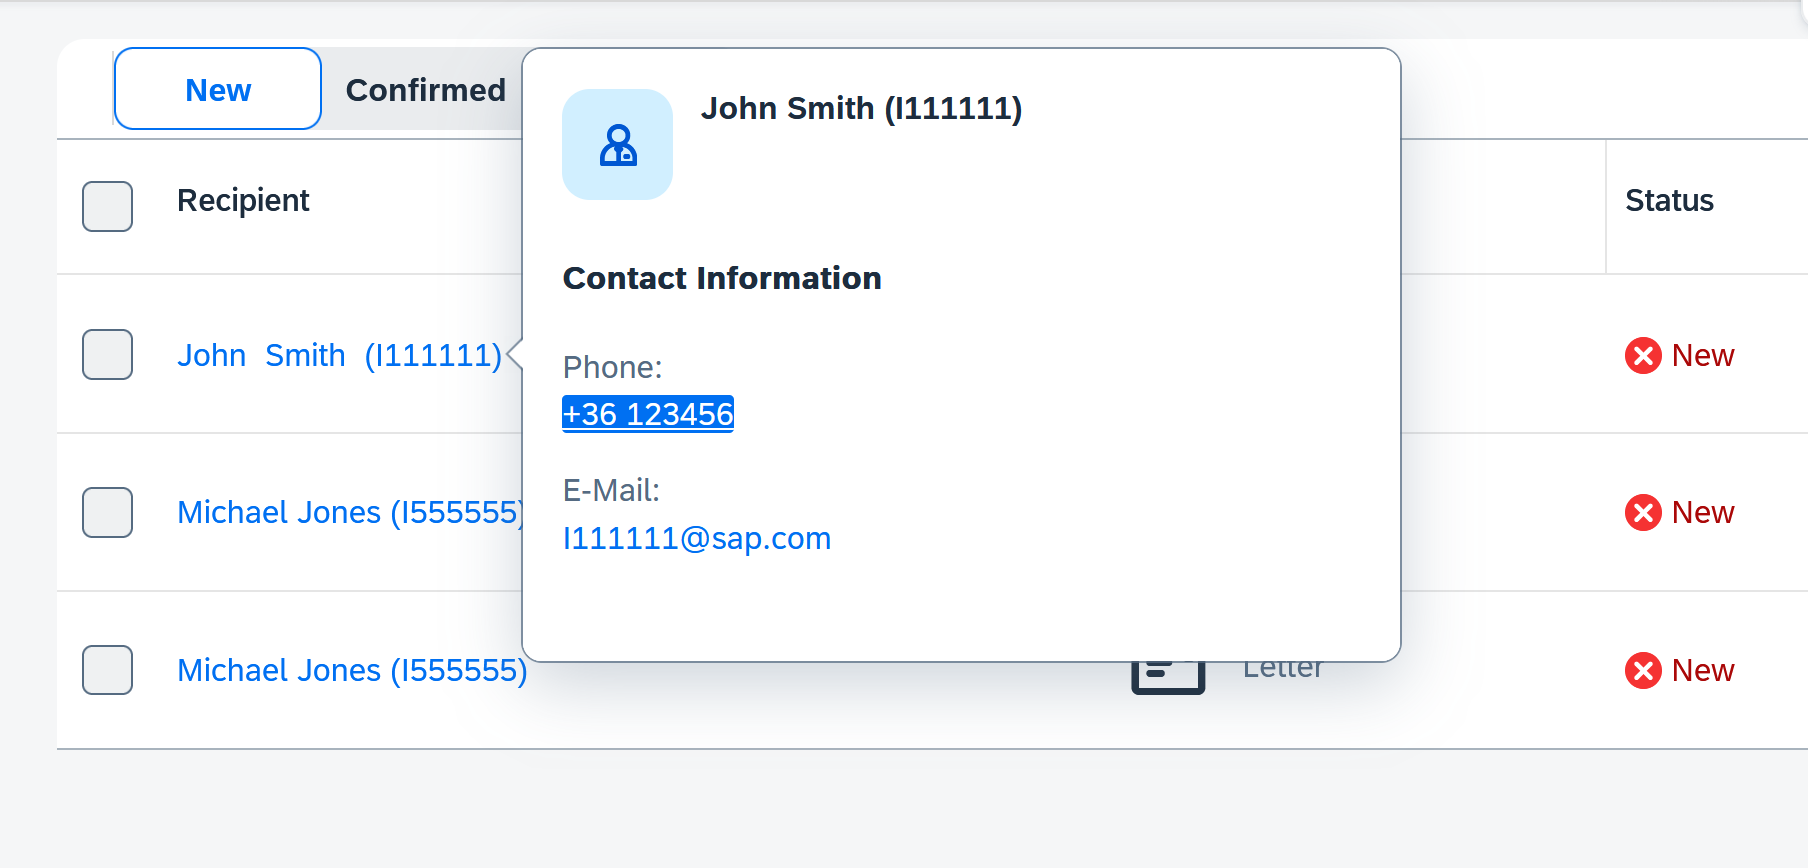
\includegraphics[height=200pt]{images/user_doc/managePack/ReportScreen/browse/contactcard.png}
	\caption{Manage Packages Report Screen - Report List - Contact Card Show Case}
	\label{fig:MPReportCOntactCard}
\end{figure}

Further details of a package can be checked by clicking at the package list items. On click, one is navigated to the "Package Detail Screen" displaying \textbf{Basic}, \textbf{General Data} and \textbf{Administrative Data} of the package.

In case the contact info of recipient or receptionist is needed, a contact card can be displayed by clicking on the person.

\begin{figure}[H]
	\centering
	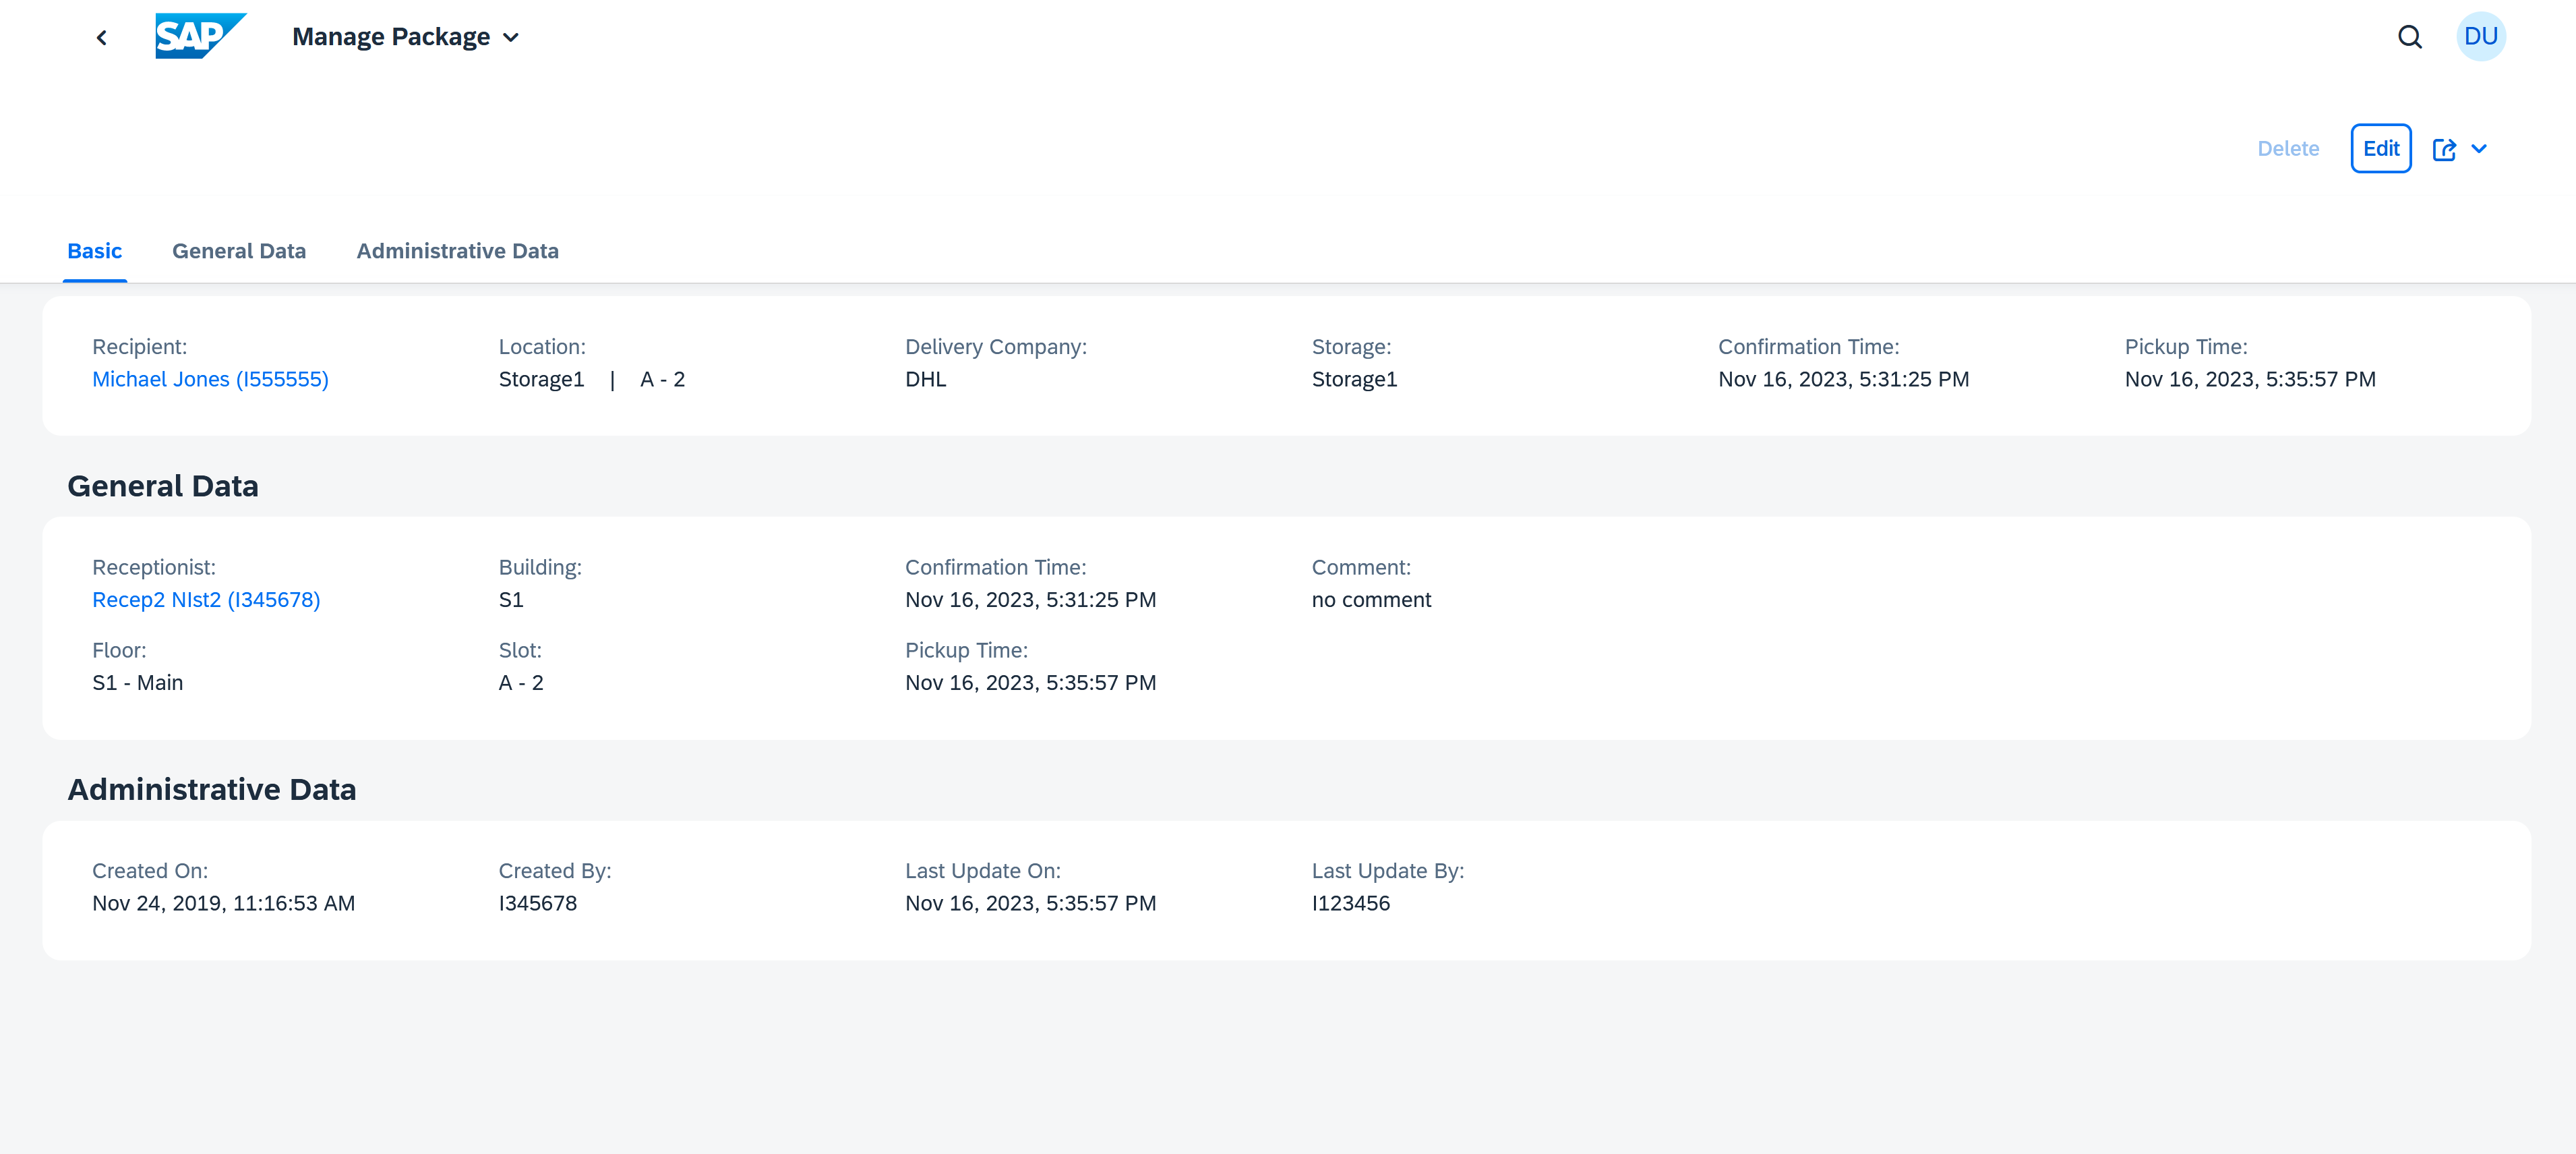
\includegraphics[height=200pt]{images/user_doc/managePack/DetailScreen/browse/overview.png}
	\caption{Manage Packages Detail Screen - Overview}
	\label{fig:MPReportCOntactCard}
\end{figure}

\begin{figure}[H]
	\centering
	\subcaptionbox{Receptionist}{
		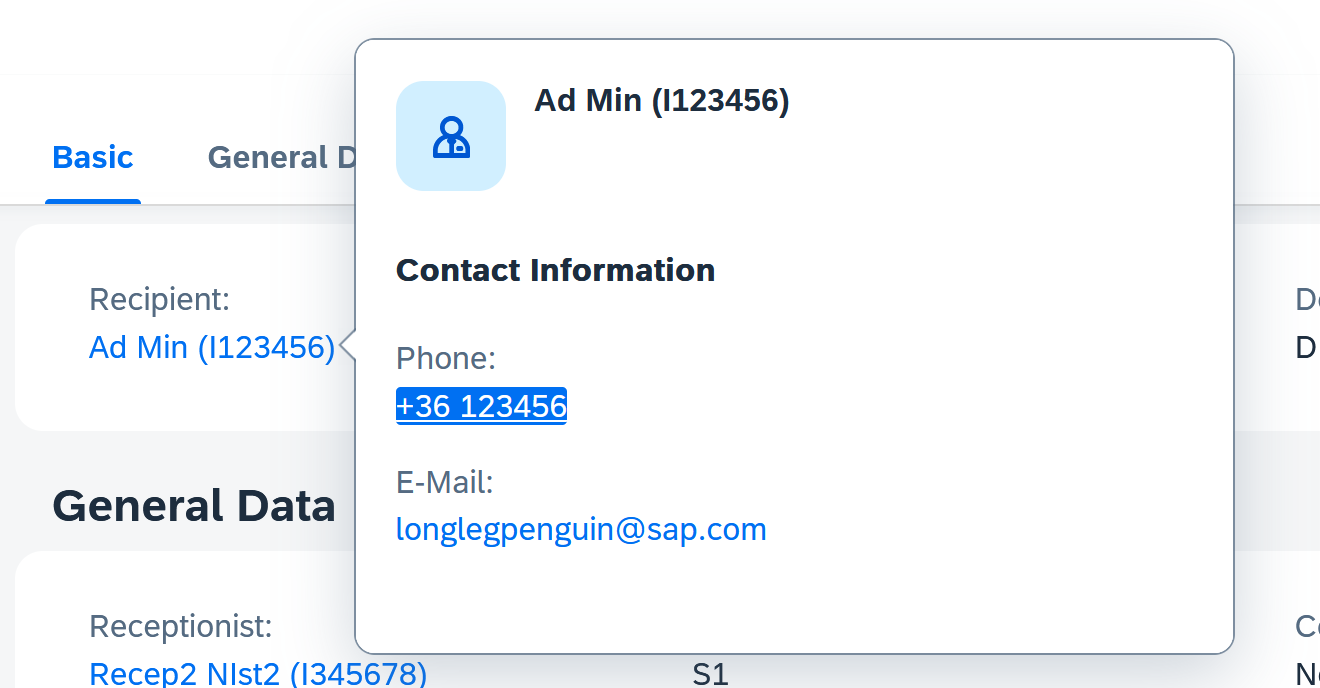
\includegraphics[width=0.45\linewidth]{images/user_doc/managePack/DetailScreen/browse/contactcard_recep.png}}
	\hspace{5pt}
	\subcaptionbox{Recipient}{
		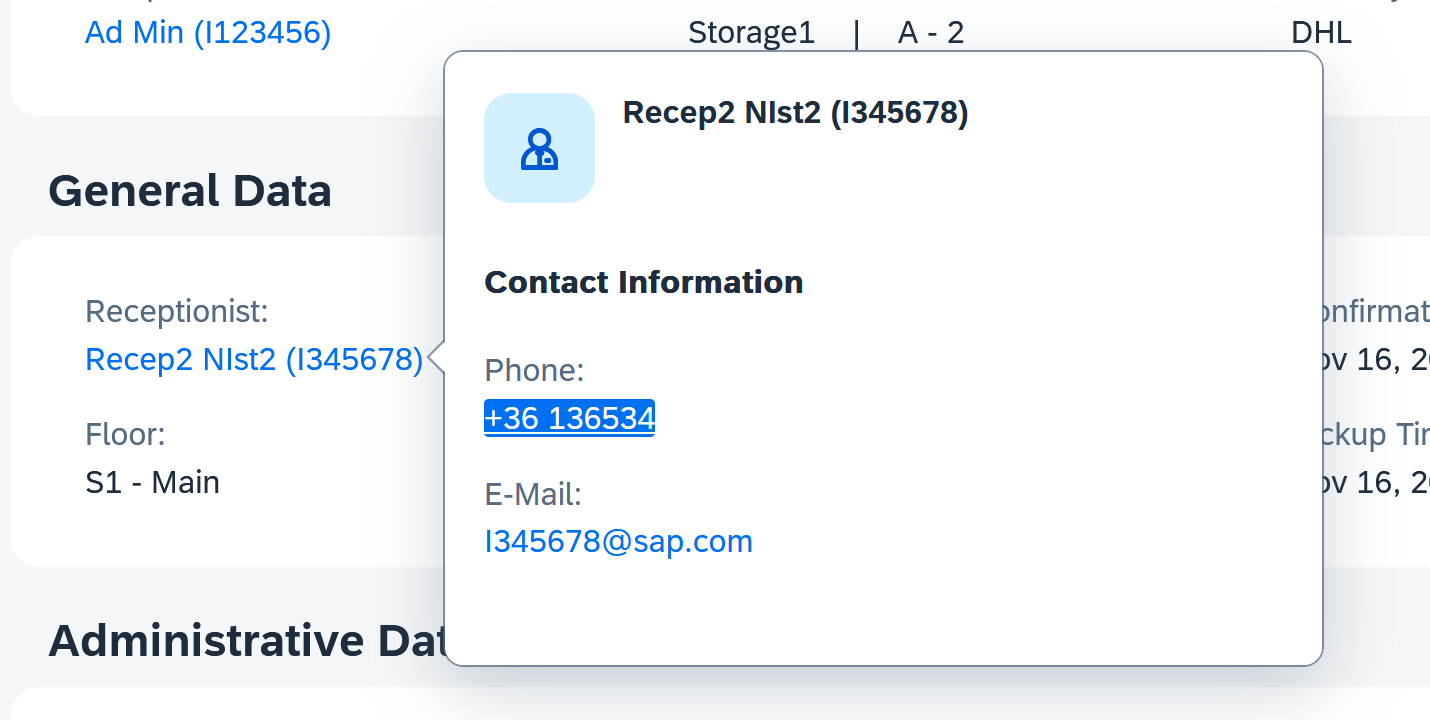
\includegraphics[width=0.45\linewidth]{images/user_doc/managePack/DetailScreen/browse/contactcard_user.png}}
    \caption{Manage Packages Detail Screen - Contact Card}
	\label{fig:MPObjectContactCard}
\end{figure}

\subsubsection{Confirm}

Confirm a package happens after a \textbf{Receptionist} registered a delivered package when the \textbf{Receptionist} would like to allocate the package a storage slot. Only packages with \textit{new} status can be confirmed. One to many \textit{new} packages can be confirmed at a single time.

The \textbf{Confirm} button at the middle control part is used to trigger the confirm action. It is inactivated until the following conditions are all full filled:

\begin{compactenum}
    \item At the \textbf{New} variant.
    \item At least one \textit{new} package is selected.
\end{compactenum}

Once the \textbf{Receptionist} selected the packages, the \textbf{Confirm} button is activated and clicked, a dialog pops up for the \textbf{Receptionist} to allocate a slot for the package(s). One should select the storage first from the \textbf{Storage} drop down list and then the slot from the \textbf{Slot} drop down list. The \textbf{Slot} drop down shows always the available slots under the selected storage.

After selected the slot, if one clicks "Cancel", nothing will happen and dialog will be closed. If one clicks "Confirm", the packages will be confirmed (i.e. filled with the selected slot info and status changed to confirmed). The dialog will be closed, a message toast indicates the success confirm and the package(s) will be moved from the current \textbf{New} variant to \textbf{Confirmed} Variant.

At this point, the package(s) are ready to be picked up, by employee through \textbf{Package Pickup} application or by \textbf{Receptionist} using the pickup backup function of this application.



\subsubsection{Pickup}
\subsubsection{Delete}
\subsubsection{Edit}
\pagebreak

\section{Facility Manager}

As a logged in \textbf{Facility Manager}, one is granted to access the two applications under the \textbf{Administration} section, namely \textbf{Manage Companies} and \textbf{Manage Storage}. One can quick jump to the section by left clicking the "Administration" tab. One can enter the application by left click the tiles.

\begin{figure}[H]
	\centering
	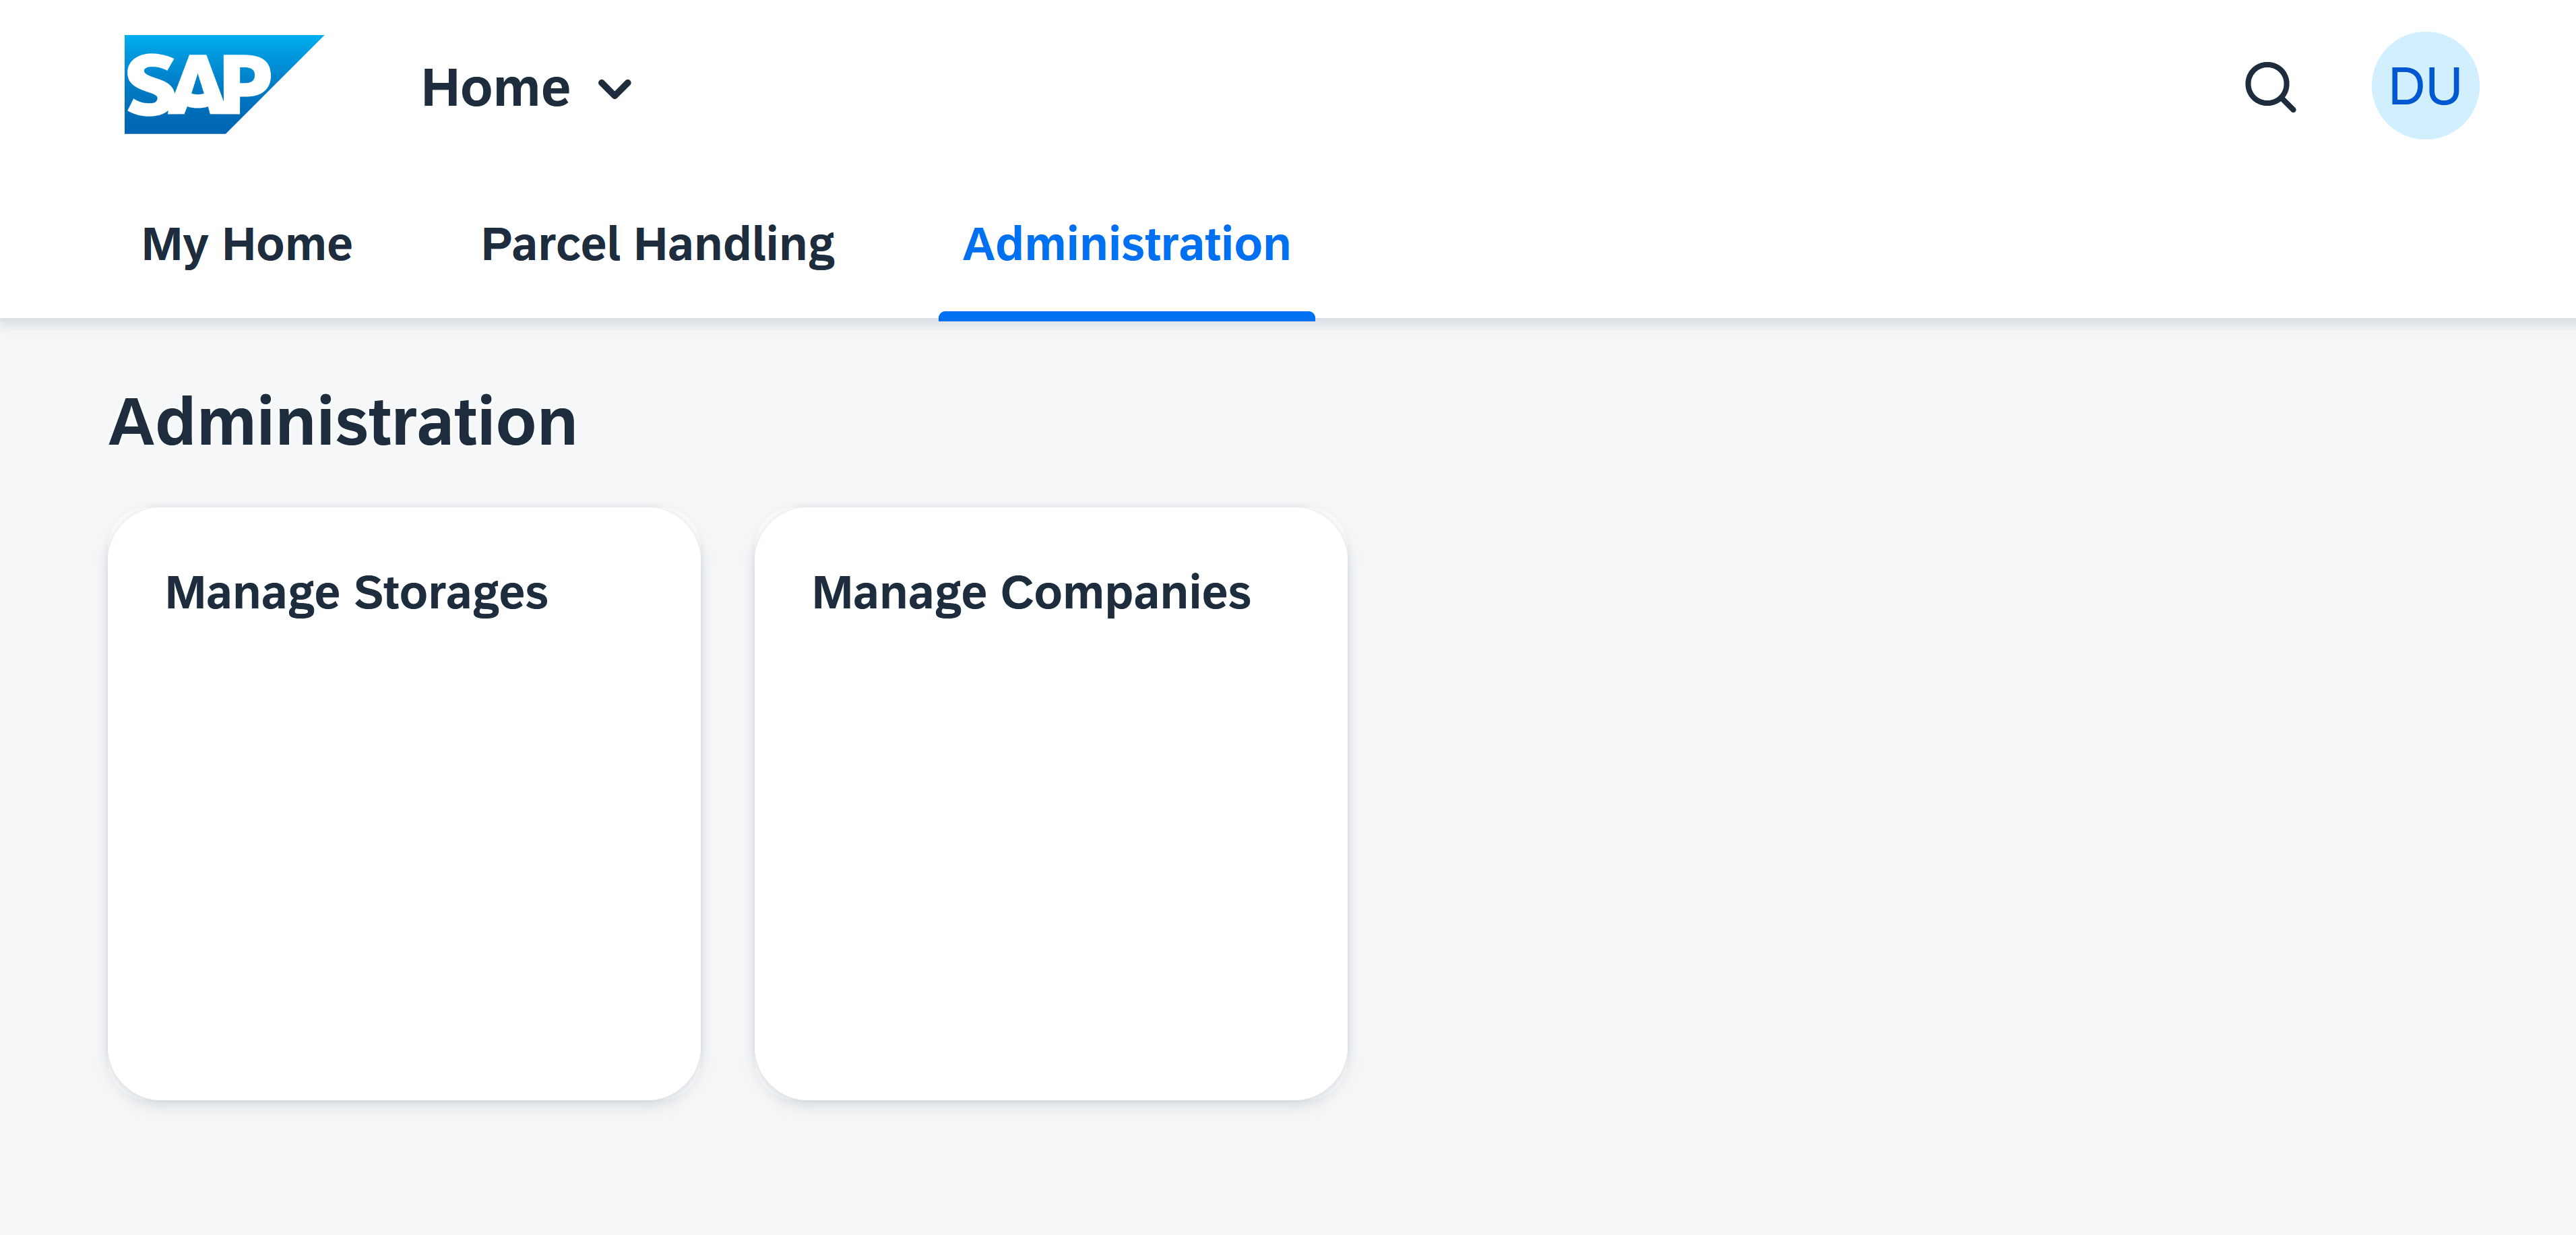
\includegraphics[width=1\linewidth]{images/user_doc/overviews/AdminTab.png}
	\caption{Administration Applications}
	\label{fig:AdministrationApplications}
\end{figure}


\subsection{Manage Companies}


\subsection{Manage Storage}


\section{Administrator}
As a logged in \textbf{Administrator}, one has access to all the 6 applications. One shall move backward to dedicated sections depends on the needs. 